\documentclass{article}
\usepackage[utf8]{inputenc}
\usepackage[T1]{fontenc}

\title{Appunti di Introduzione all'Intelligenza Artificiale Unipi - 2 Parte}
\author{Raffaele Apetino}
\date{Marzo 2020}

\usepackage{natbib}
\usepackage{graphicx}
\usepackage[margin=3cm]{geometry}
\usepackage{amssymb}
\usepackage{xcolor}
\usepackage{proof}
\usepackage{float}
\usepackage{tipa}

\begin{document}

\maketitle

\tableofcontents{}
\clearpage

%Lezione 6
\section{Giochi con avversario}
Il modello base a cui ci siamo affidati fin'ora è realizzato su ambienti osservabili, deterministici e con utente singolo. Nella prima parte del corso abbiamo visto che esistono gli ambienti multi-agente, in cui un agente deve tenere conto anche delle azioni degli altri agenti che lo circondano. I giochi con avversario\footnote{due giocatori, turni alterni, a somma zero (se uno vince, l'altro perde)} si basano su ambienti deterministici multi-agente competitivi, in particolare su un ambiente reso strategico a causa della presenza di un avversario. \newline 
Vedremo i problemi di soddisfacimento dei vincoli (CSP) in cui lo stato ha una struttura fattorizzata. Vedremo che nei sistemi basati su conoscenza lo stato è una "base di conoscenza" (KB) a cui rivolgere domande sul mondo rappresentato in un linguaggio espressivo come il PROP (calcolo proposizionale) o FOL (logica del primo ordine). 

\subsection{Ciclo Pianifica-Agisci-Percepisci}
Ci troviamo nel caso in cui abbiamo due agenti che agiscono a turno, si pianifica considerando le possibili risposte dell'avversario e le risposte alla possibile sua risposta e così via. Una volta decisa la mossa migliore da fare, si agisce, si percepisce la mossa dell'avversario e infine si ri-pianifica la mossa. \newline 
La decisione ottima teorica è definita come la mossa migliore in un gioco con uno spazio di ricerca completamente esplorabile (per trovarla utilizzeremo l'algoritmo MIN-MAX). E' possibile che ci troveremo in situazioni in cui a causa della complessità non sarà possibile eseguire una esplorazione esaustiva dello spazio. Sfrutteremo, inoltre, tecniche di ottimizzazione della ricerca (algoritmo ALFA-BETA).

\subsection{Definizione spazio degli stati}
Un gioco può essere definito formalmente come una sorta di problema di ricerca con i seguenti elementi:
\begin{itemize}
    \item Stati: configurazioni del gioco
    \item Stato iniziale: configurazione iniziale del gioco
    \item Player(s): a chi tocca eseguire l'azione nello stato s
    \item Actions(s): mosse legali in s
    \item Result(s,a): stato risultante dopo aver eseguito la mossa a nello stato s (modello di transizione)
    \item Terminal-Test(s): determina la fine del gioco, controlla che s sia lo stato terminale (e quindi il gioco finito)
    \item Utility(s,p): funzione di utilità (chiamata anche funzione obiettivo o funzione pay-off) che restituisce un valore numerico che valuta gli stati terminali del gioco per p (ad esempio somma di punteggi ecc...)
\end{itemize}

\subsection{Game Tree}
Lo stato iniziale insieme alle funzioni Actions e Result definiscono l'albero di gioco (Game Tree). É un albero dove ogni nodo é uno stato del gioco e i rami definiscono una mossa. Ogni foglia definisce uno stato terminale del gioco con associato di un valore di utilità definito dalla funzione Utility. \newline
Il prossimo esempio che vedremo é il gioco del Tris, i due giocatori si alternano tra MAX che posiziona le X e MIN che posiziona i cerchi, fino a che si arriva ad una delle foglie dell'albero che rappresentano un nodo terminale.
\clearpage

\subsection{Algoritmo MIN-MAX}
\begin{figure}[H]
\centering
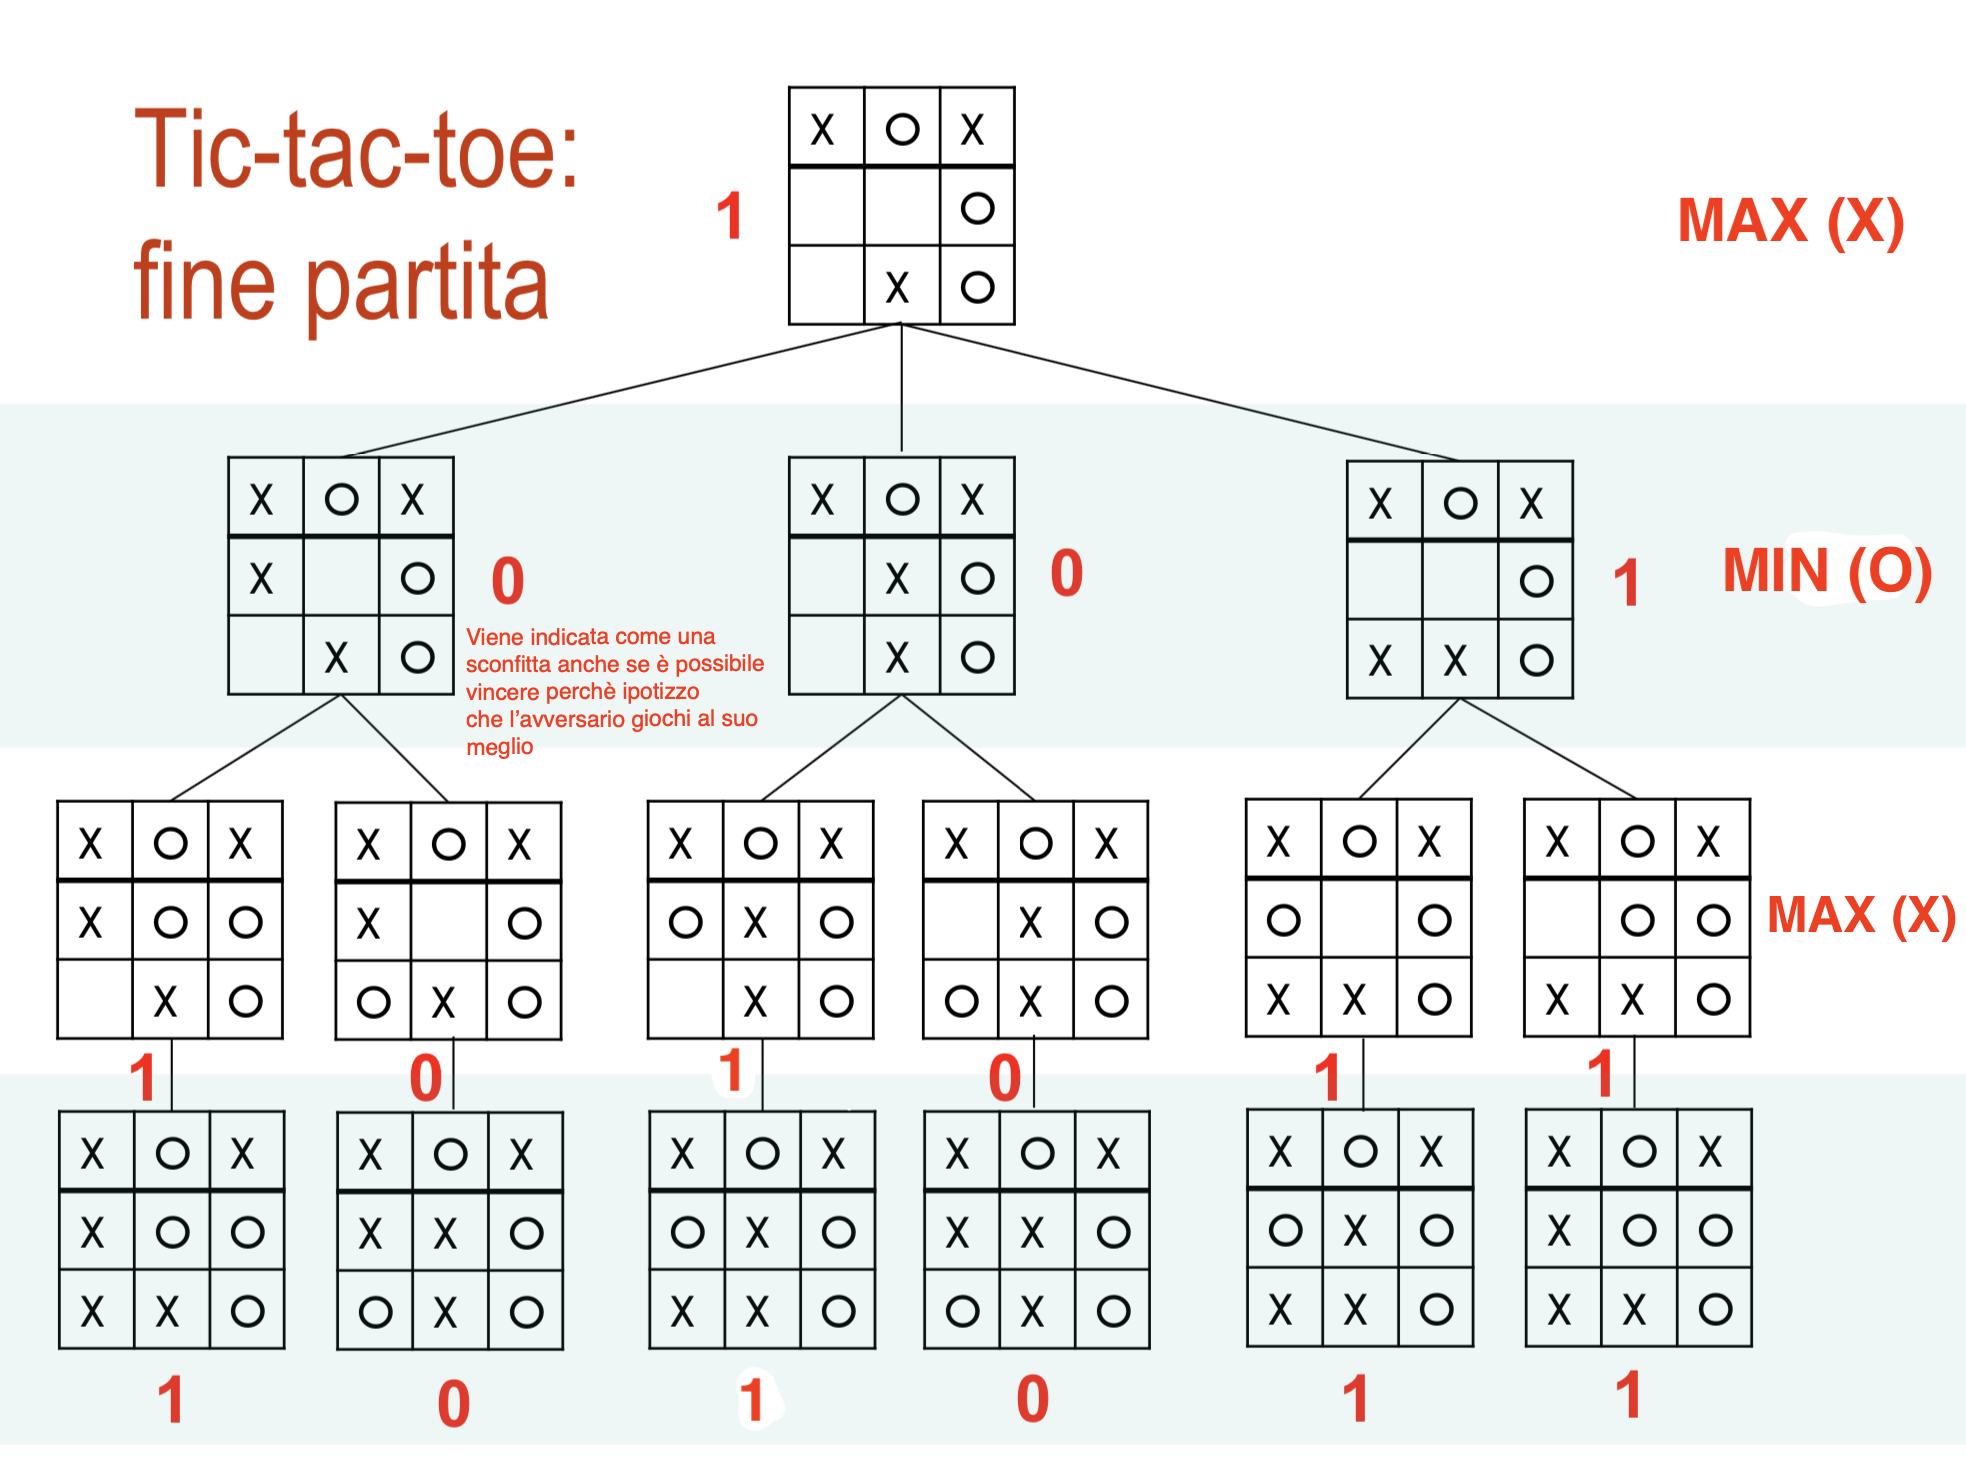
\includegraphics[scale=0.45]{Images/minmaxtictactoe.png}
\caption{Albero parziale costruito dall'algoritmo MIN-MAX}
\end{figure}
L'albero creato da MIN-MAX é molto simile ad un albero AND-OR, in cui i nodi MAX hanno il ruolo di OR e MIN quello di AND.

\subsubsection{Come si calcola il valore MIN-MAX?}
Dato un albero di gioco, la strategia ottima é determinata dal valore "MINIMAX" di ogni nodo:
\begin{quote}
MINIMAX(s) =
\begin{itemize}
    \item if (Terminal-Test(s) == true) Utility(s,MAX)
    \item if (Player(s) == MAX) $max_{a \in Actions(s)}(MINIMAX(Result(s,a)))$
    \item if (Player(s) == MIN) $min_{a \in Actions(s)}(MINIMAX(Result(s,a)))$
\end{itemize}
\end{quote}
Ovviamente il valore MINIMAX di uno stato terminale é la sua utilitá. Altrimenti, per ogni possibile azione (e quindi ramo), MAX preferisce spostarsi sui nodi in cui il valore MINIMAX é massimo, MIN su quelli di valore minimo. \newline
L'albero di gioco conviene esplorarlo in profondità, perché in ampiezza occuperei troppa memoria, ma soprattutto a noi interessa trovare uno dei tanti percorsi di vincita.

\begin{figure}[H]
\centering
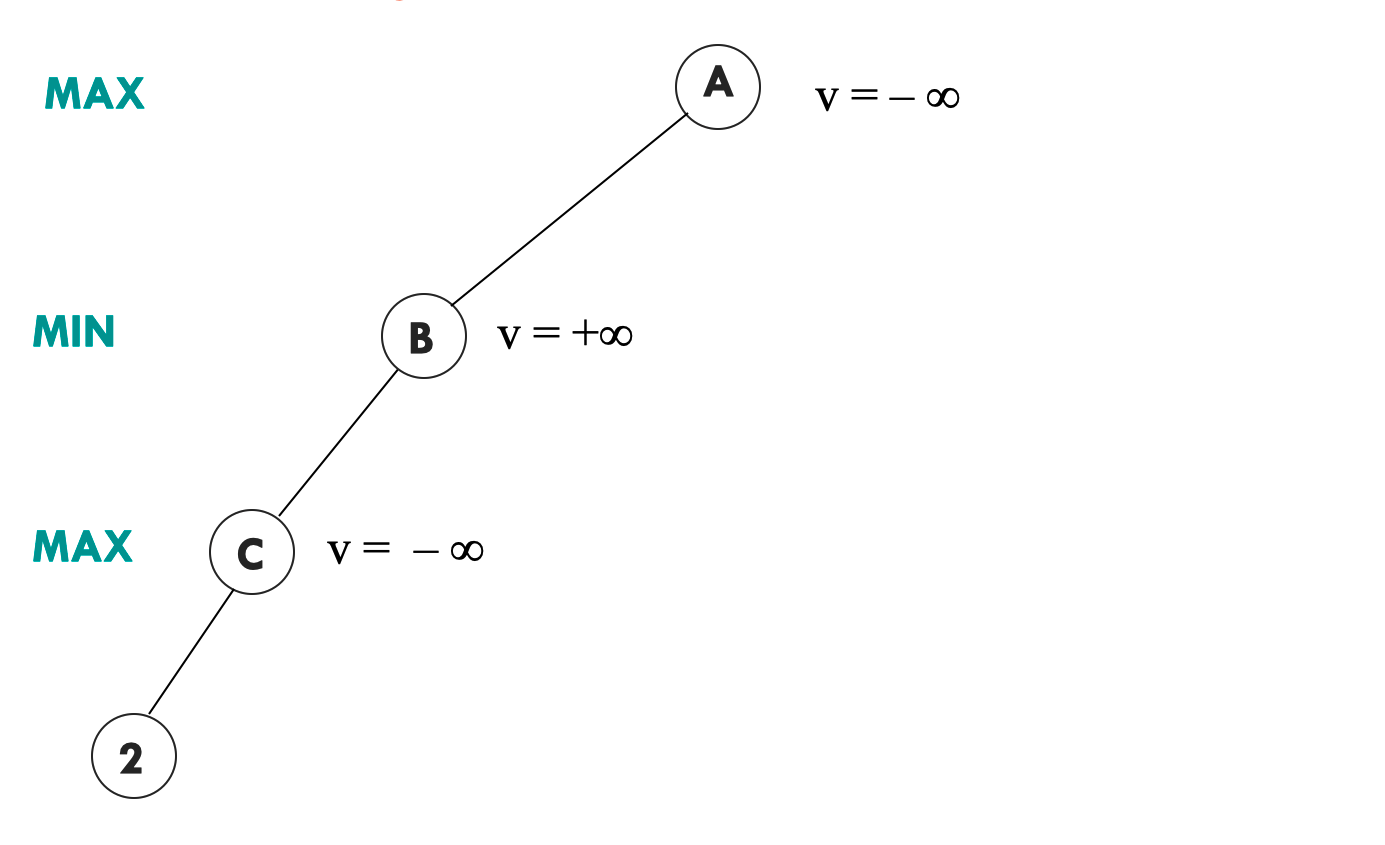
\includegraphics[scale=0.15]{Images/minmaxaction1.png}
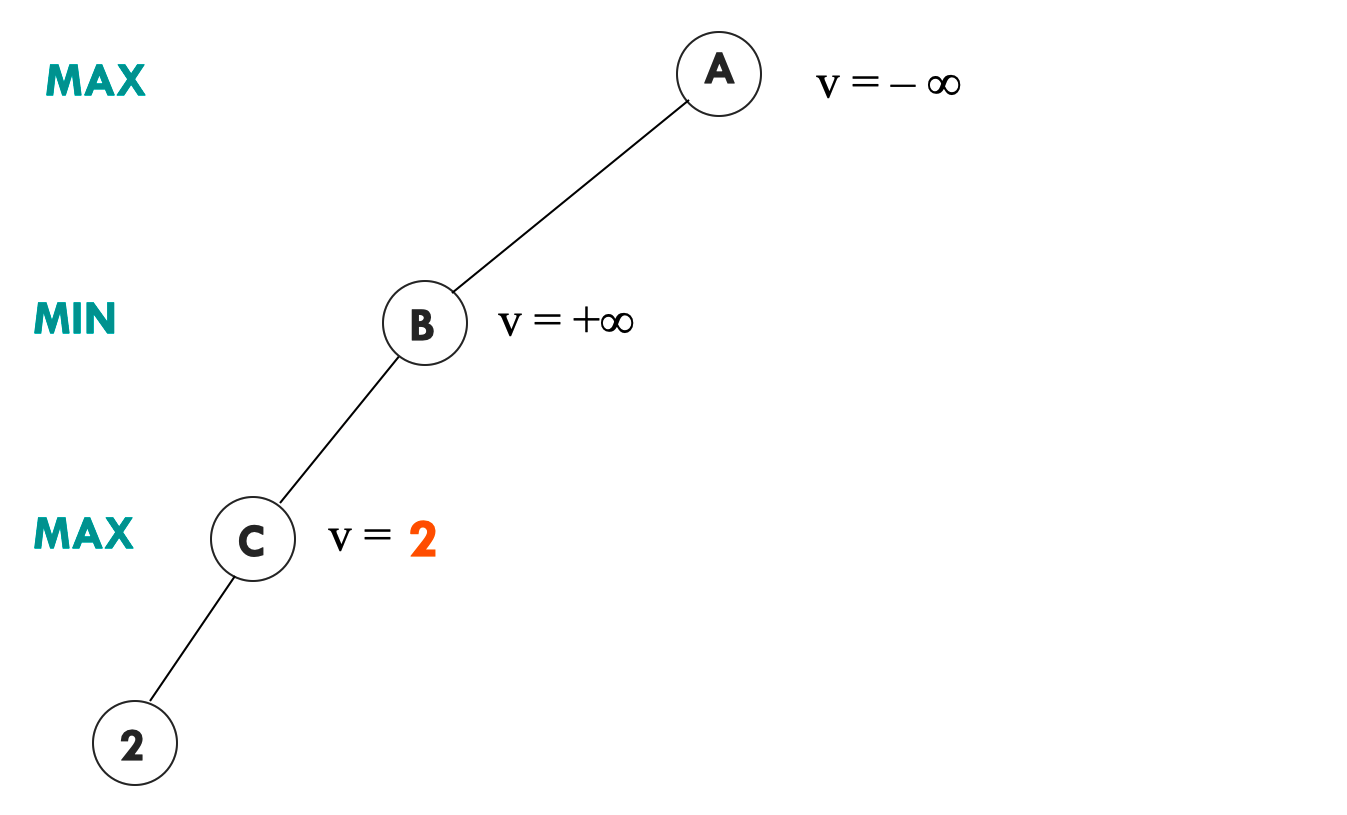
\includegraphics[scale=0.15]{Images/minmaxaction2.png}
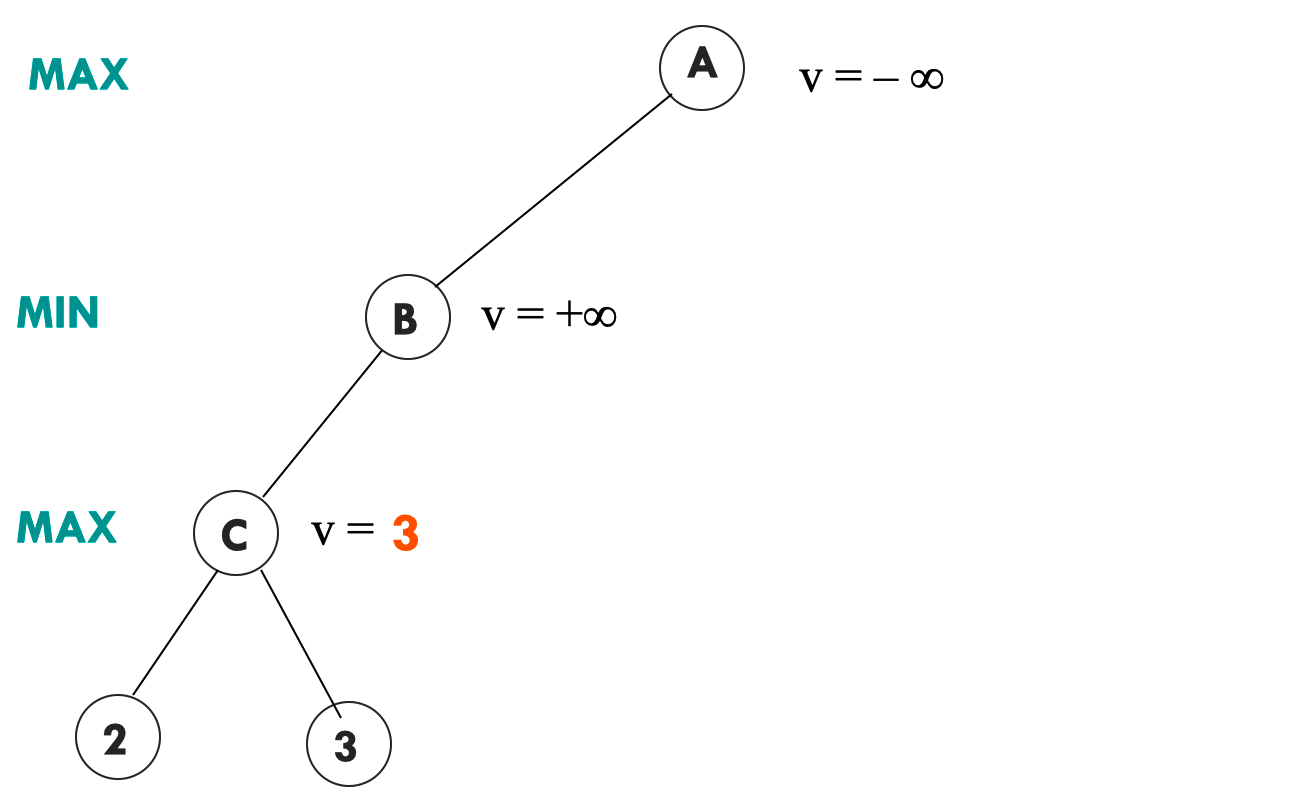
\includegraphics[scale=0.15]{Images/minmaxaction3.png}
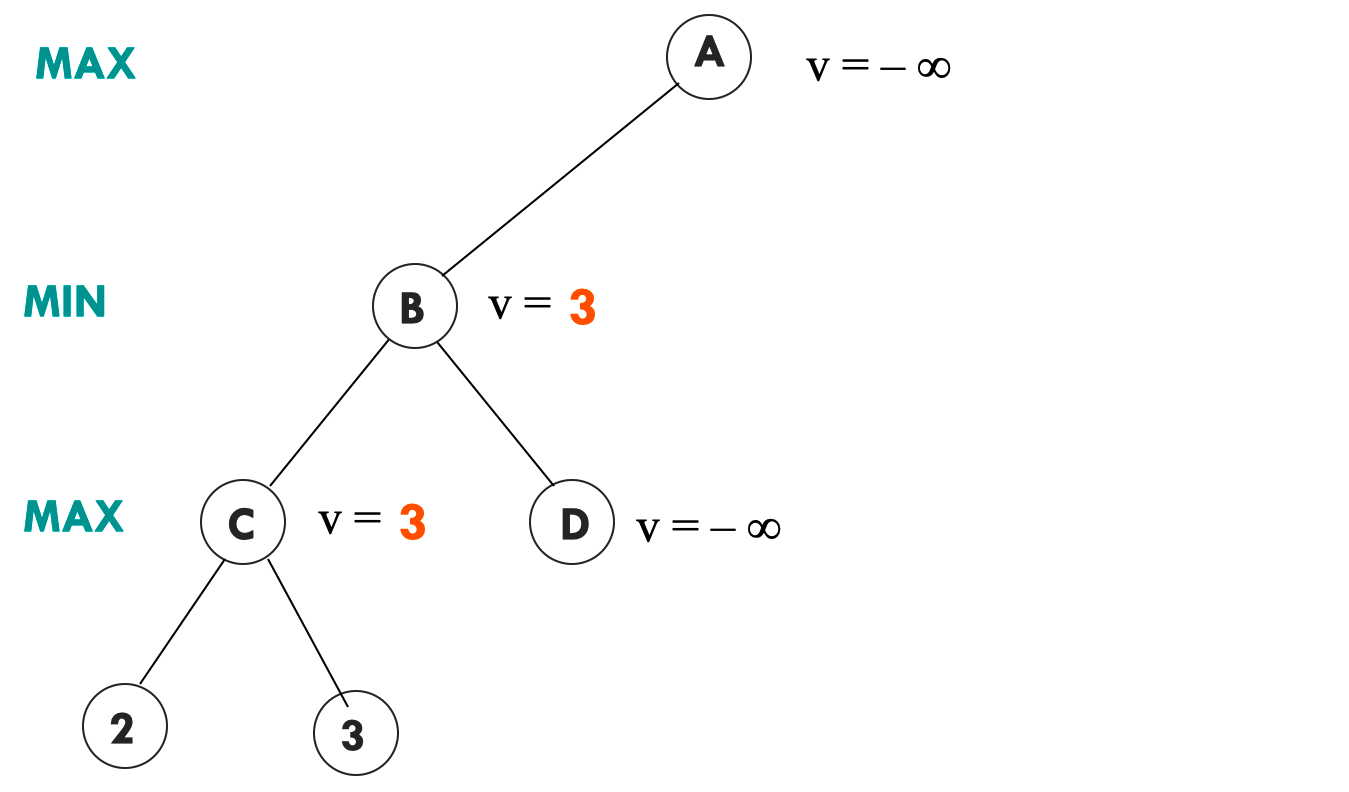
\includegraphics[scale=0.15]{Images/minmaxaction4.png}
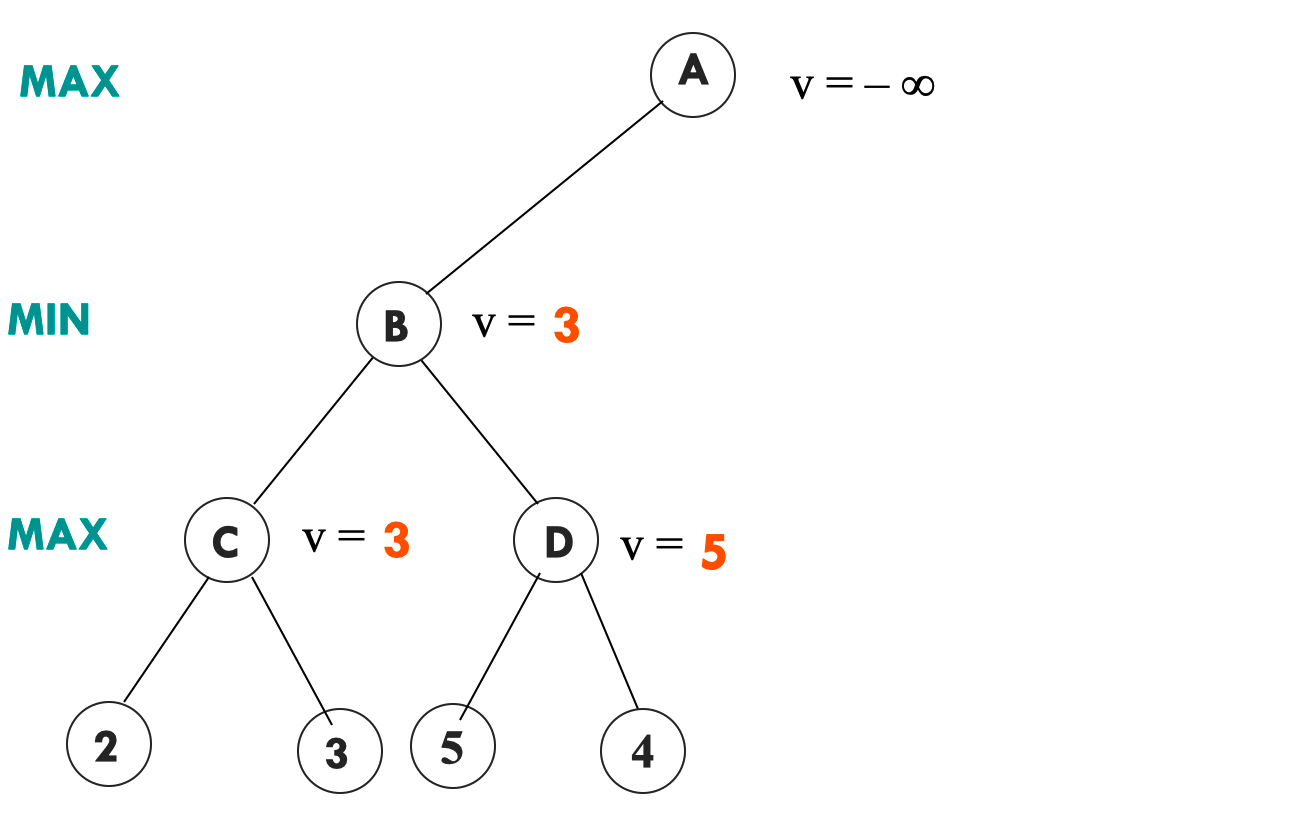
\includegraphics[scale=0.15]{Images/minmaxaction5.png}
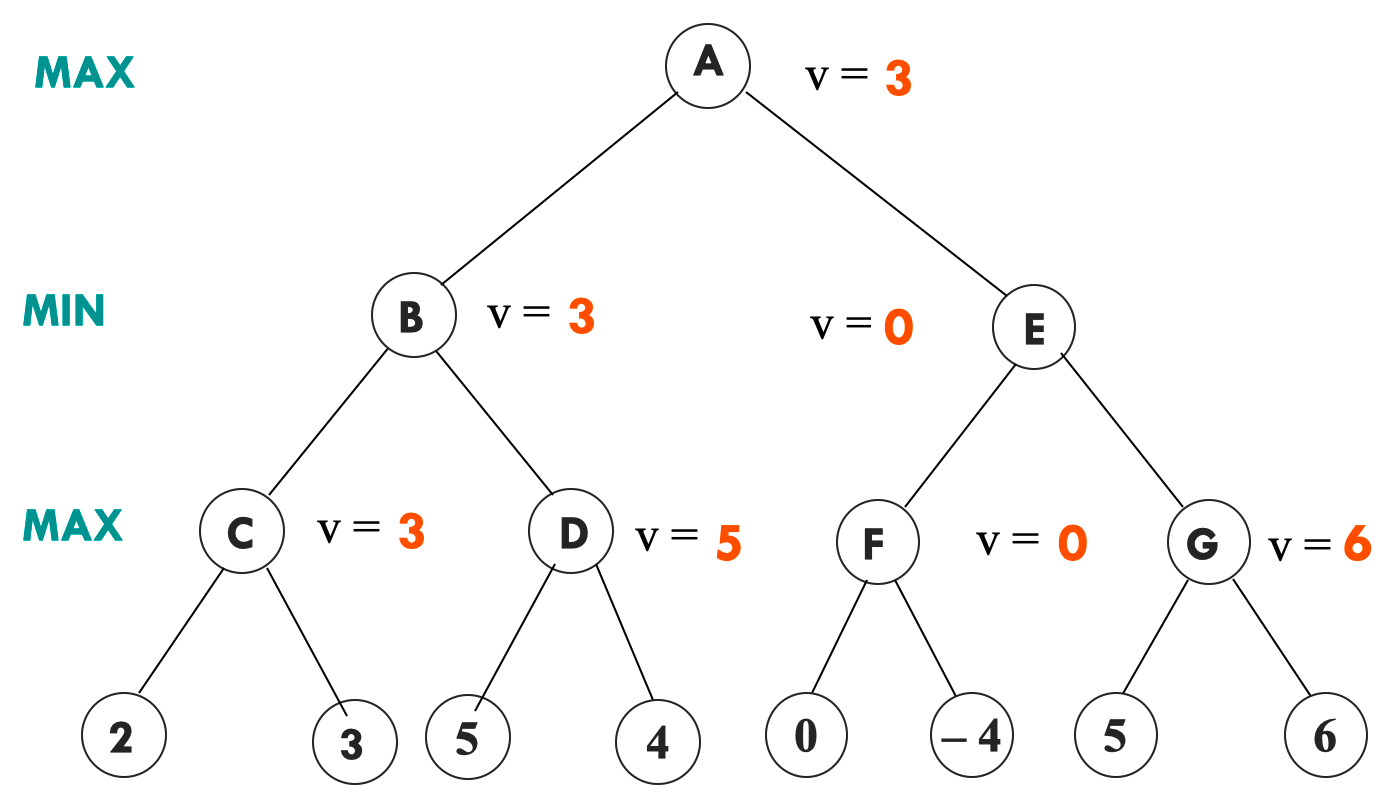
\includegraphics[scale=0.15]{Images/minmaxaction6.png}
\caption{Algoritmo MIN-MAX in azione}
\end{figure}
\subsubsection{Costo MIN-MAX}
\begin{itemize}
    \item Tempo: $O(b^m)$
    \item Spazio: $O(m)$
\end{itemize}
In giochi complessi come gli scacchi abbiamo un albero di ricerca molto grande $35^{100}$ (35 mosse in media, 100 mosse in media per ogni partita quindi 50 mosse per player), purtroppo anche mantenendo solo i nodi distinti, il grafo di ricerca rimane ampio: $(10^{40})$ nodi! É quindi improponibile una esplorazione sistematica, se non per giochi veramente semplici. Troviamo la necessità di far uso di euristiche per stimare il valore di uno stato del gioco.

\subsection{Algoritmo MIN-MAX euristico (con orizzonte)}
Nei casi più complessi quindi occorre usare una funzione di valutazione euristica dello stato Eval(s). La strategia che applicheremo sarà quella di espandere l'albero di ricerca un certo numero di "d" livelli, si valutano gli stati ottenuti e si propaga indietro il risultato con la regola del MAX e MIN. Quindi al posto di eseguire un Terminal-Test eseguiremo un CutOff-Test che ci dirà quando eseguire la funzione di valutazione.

\subsubsection{Come si calcola il valore MINIMAX euristico (H-MINIMAX)?}
H-MINIMAX(s,d) =
\begin{itemize}
    \item if (CutOff-Test(s,d) == true) Eval(s)
    \item if (Player(s) == MAX) $max_{a \in Actions(s)}H-MINIMAX(Result(s,a), d+1)$
    \item if (Player(s) == MIN) $min_{a \in Actions(s)}H-MINIMAX(Result(s,a), d+1)$
\end{itemize}

\subsubsection{Esempio H-MIN-MAX in Tic-Tac-Toe}
La funzione di valutazione Eval(s) è una stima dell'utilità attesa a partire da una certa posizione nel gioco. La "qualità" della funzione è fondamentale: deve essere consistente con la vera utilità se applicata a stati terminali del gioco (deve mantenere lo stesso ordinamento dei nodi), deve essere efficiente da calcolare (immaginiamo dei giochi a tempo) ma deve anche essere fortemente correlata alle probabilità di vittoria. \newline 
Usiamo come funzione di valutazione la differenza tra le X(s) righe aperte per X e O(s) righe aperte per O. La nostra euristica sarà: Eval(s) = X(s) - O(s)
\begin{figure}[H]
\centering
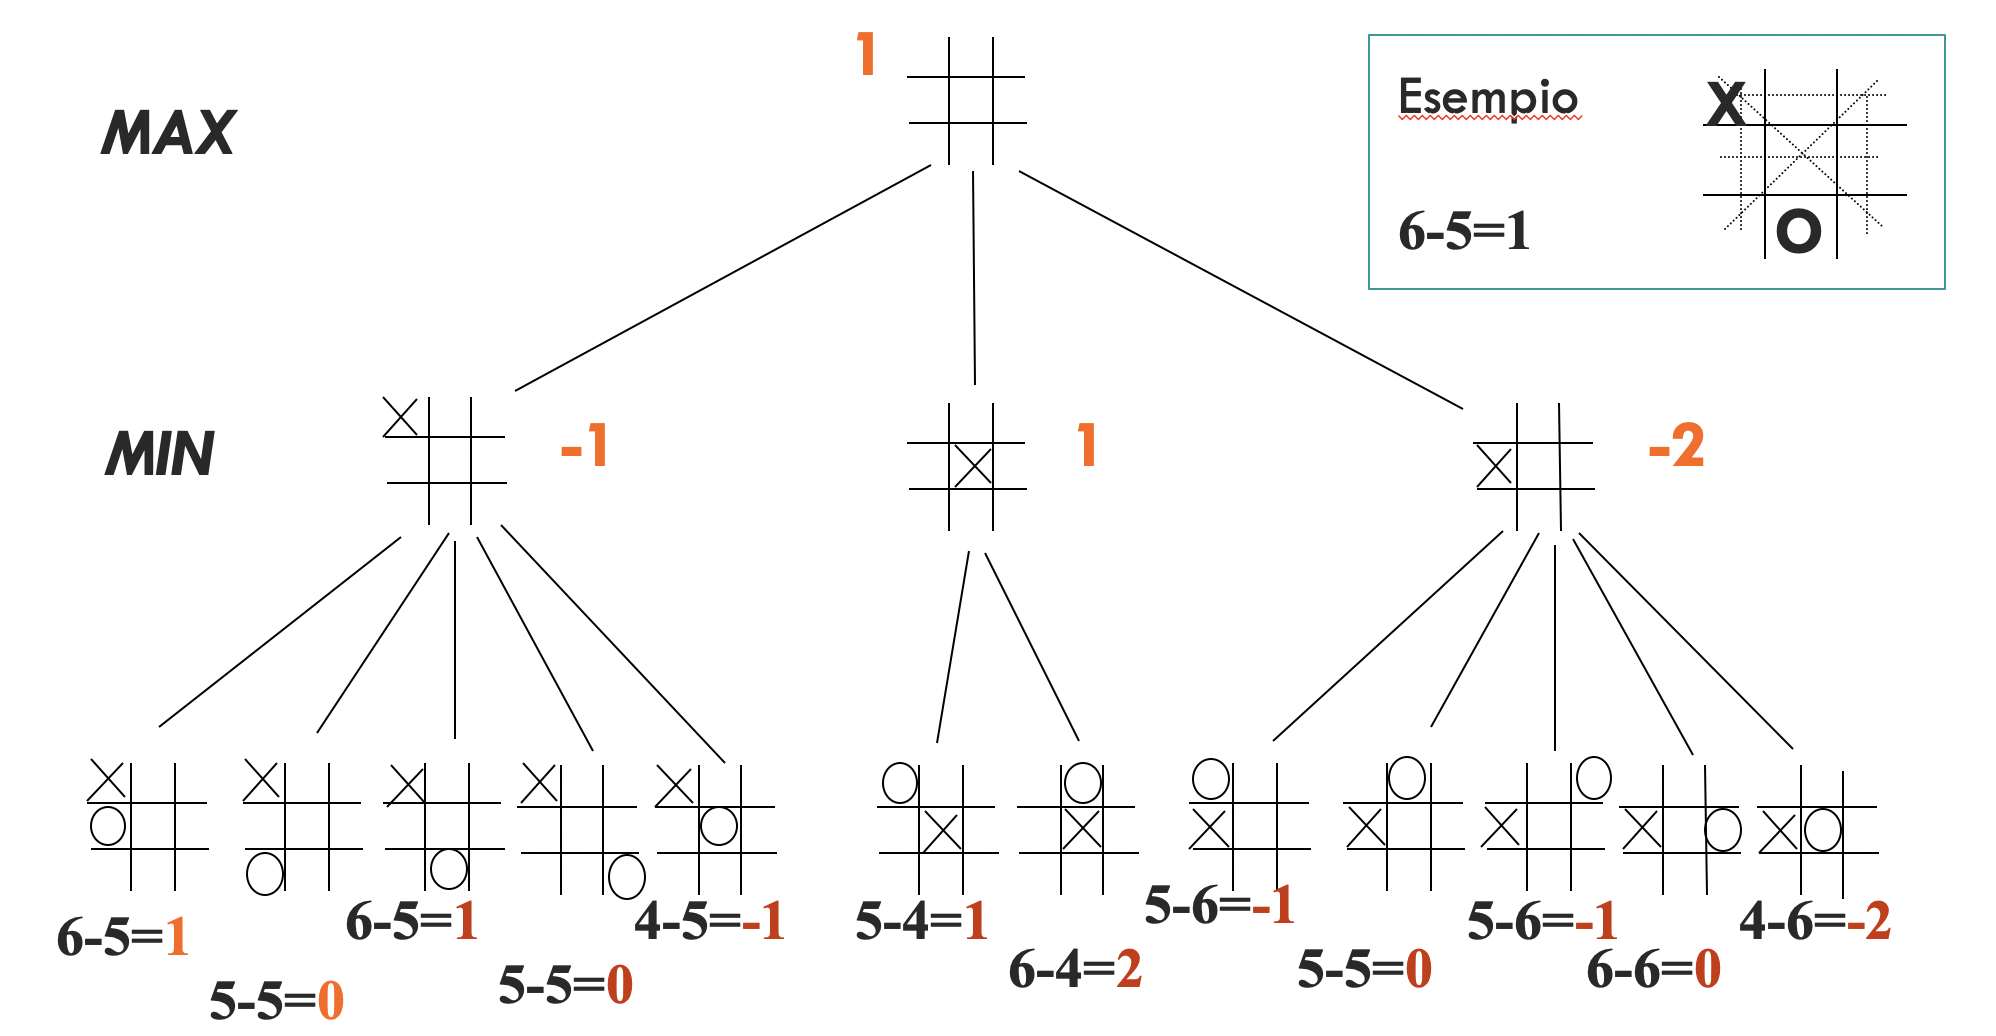
\includegraphics[scale=0.4]{Images/minmaxeuristico.png}
\caption{Algoritmo MIN-MAX euristico in azione}
\end{figure}

\subsection{Problemi con MIN-MAX}
\begin{itemize}
    \item Stati non quiescenti: l’esplorazione fino ad un certo livello può mostrare una situazione molto vantaggiosa, ma alla mossa successiva la situazione può peggiorare esponenzialmente. La soluzione da applicare è la funzione di valutazione a stati quiescenti, cioè stati in cui Eval(s) non è soggetta a mutamenti repentini (questo implica la ricerca di quiescenza).
    \item Effetto orizzonte: può succedere che vengano privilegiate mosse diversive che hanno il solo effetto di spingere il problema oltre l’orizzonte. Una sorta di serie di mosse che non fanno altro che "scappare" dal problema il più possibile, magari ritrovandosi in un loop infinito.
\end{itemize}

\subsection{Ottimizzazione MIN-MAX}
E' necessario esplorare ogni cammino? NO! si può sfruttare un metodo per dimezzare la ricerca pur mantenendo una decisione della prossima mossa corretta (Potatura ALFA-BETA).

\subsection{Potatura ALFA-BETA}
Il problema principale della ricerca MIN-MAX é il numero di stati che cresce esponenzialmente in relazione alla profonditá dell'albero. Purtroppo non possiamo eliminare l'esponente, ma possiamo dimezzarlo. \newline
ALFA-BETA é una tecnica di potatura per ridurre l’esplorazione dello spazio di ricerca in algoritmi MIN-MAX. L'idea è che si vada avanti in profondità fino al livello desiderato, si propaghino indietro i valori e a questo punto si decida se si può abbandonare l’esplorazione nel sotto-albero. Sfruttiamo due valori "MaxValue" ($\alpha$) e "MinValue" ($\beta$) rispettivamente inizializzati a $\alpha=-\infty$ e $\beta=+\infty$. Rappresentano rispettivamente la migliore alternativa per MAX e per MIN fino a quel momento. \newline
I tagli del sottoalbero avvengono quando nel propagare indietro troviamo: 
\begin{itemize}
    \item $v \geq \beta$ per i nodi MAX (taglio $\beta$)
    \item $v \leq \alpha$ per i nodi MIN (taglio $\alpha$) 
\end{itemize}
\begin{figure}[H]
\centering
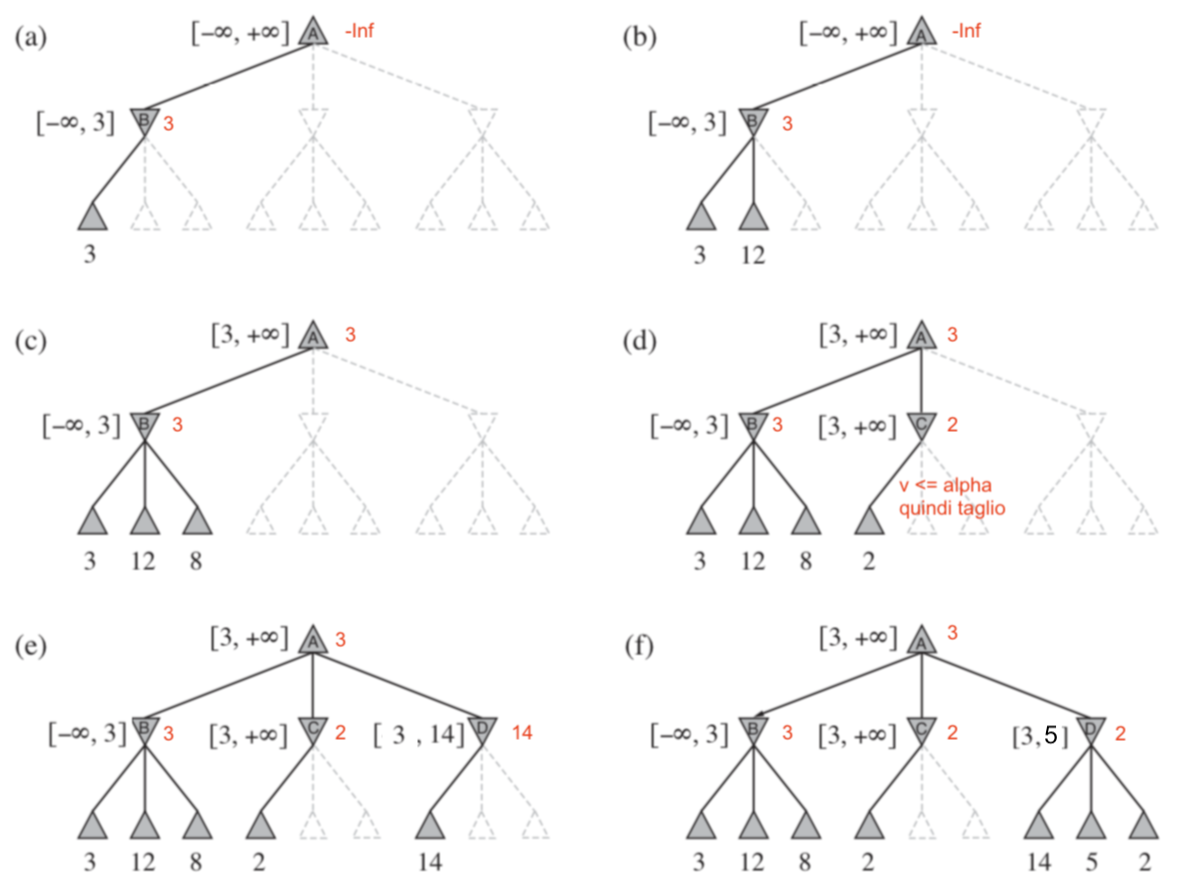
\includegraphics[scale=0.74]{Images/esempioalpha-beta.png}
\caption{Potatura ALFA-BETA in azione}
\end{figure}
\clearpage

\subsubsection{Costo potatura ALFA-BETA}
\begin{itemize}
    \item Tempo: $O(b^{m/2})$ quindi ALFA-BETA può arrivare a profondità doppia rispetto a MIN-MAX (best case)
    \item Spazio: $O(m)$
\end{itemize}

\subsubsection{Ottimizzazioni ALFA-BETA}
Quale potrebbe essere l'ordinamento ottimale? 
\begin{itemize}
    \item Ordinamento dinamico: usando un approfondimento iterativo si possono scoprire informazioni utili per l’ordinamento delle mosse da usare in una successiva iterazione (mosse killer). \newline
    Possiamo inoltre tenere in memoria una tabella delle trasposizioni, cioè per ogni stato incontrato si memorizza la sua valutazione.
    \item Potatura in avanti: si potrebbe anche eseguire una potatura in avanti, cioè esplorare solo alcune mosse ritenute promettenti e tagliare le altre (tagli probabilistici basati su esperienza).
    \item Database di mosse: possiamo inoltre sfruttare un database di mosse di apertura e chiusura. Nelle prime fasi ci sono poche mosse sensate e ben studiate, inutile esplorarle tutte, mentre per le fasi finali il computer può esplorare off-line in maniera esaustiva e ricordarsi le migliori chiusure.
\end{itemize}  

\subsection{Giochi Multiplayer}
Molti giochi permettono di far partecipare più di due giocatori. Dobbiamo modificare il singolo valore di ogni nodo con un vettore (ad esempio in foto vengono valutati allo stesso tempo 3 valori, uno per ogni giocatore).
\begin{figure}[H]
\centering
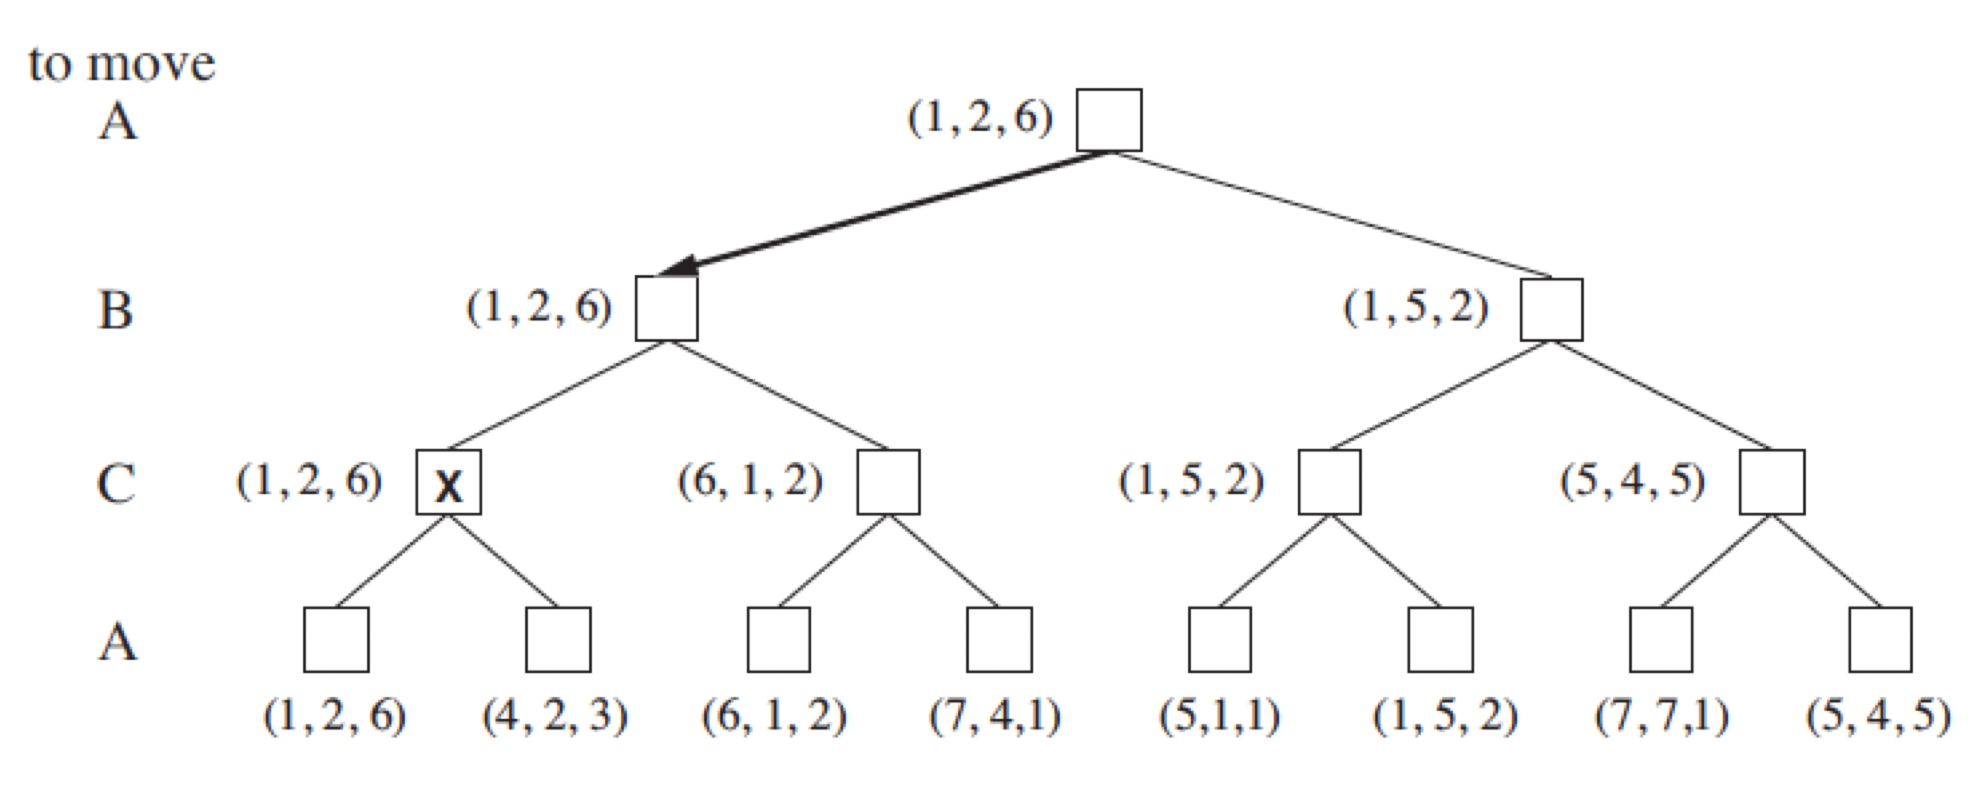
\includegraphics[scale=0.35]{Images/giochimultiplayer.png}
\caption{Giochi Multiplayer}
\end{figure}
\subsection{Giochi Complessi}
\begin{itemize}
    \item Giochi stocastici: i giochi in cui è prevista una variabile aleatoria (lancio di dadi oppure la distribuzione di carte)
    \item Giochi parzialmente osservabili: le mosse sono deterministiche ma non si conoscono gli effetti delle mosse dell'avversario. (Battaglia navale)
\end{itemize}

\section{Problemi di soddisfacimento di vincoli (CSP)}
Sono problemi con una struttura particolare che necessitano algoritmi di ricerca specializzati, si sfrutta una rappresentazione fattorizzata dello stato rendendo esplicita la sua struttura (o almeno in parte). Un problema é risolto quando ogni variabile ha un assegnamento che soddisfa tutti i vincoli. Esistono euristiche generali che si applicano a questi problemi e consentono la risoluzione anche se il problema ha dimensioni significative.
\subsection{Formulazione di problemi CSP}
\begin{itemize}
    \item Problema: descritto da tre componenti
        \begin{enumerate}
        \item X insieme di variabili
        \item D insieme di domini (ogni dominio $D_i$ é a sua volta un insieme di valori possibili per la variabile $X_i$)
        \item C insieme di vincoli (ogni vincolo $C_i$ é una coppia [variabili,relazione])
        \end{enumerate}
    \item Stato: un assegnamento parziale o completo di valori a variabili (ad esempio $X_i = v_i, X_j = v_j$...)
    \item Stato iniziale: \{\}
    \item Azioni: assegnamento di un valore ad una variabile
    \item Soluzione: un assegnamento completo della formula, dove tutte le variabili hanno un valore consistente, cioè dove tutti i vincoli sono soddisfatti
\end{itemize}

\subsubsection{Problema della colorazione di una mappa}
\begin{figure}[H]
\centering
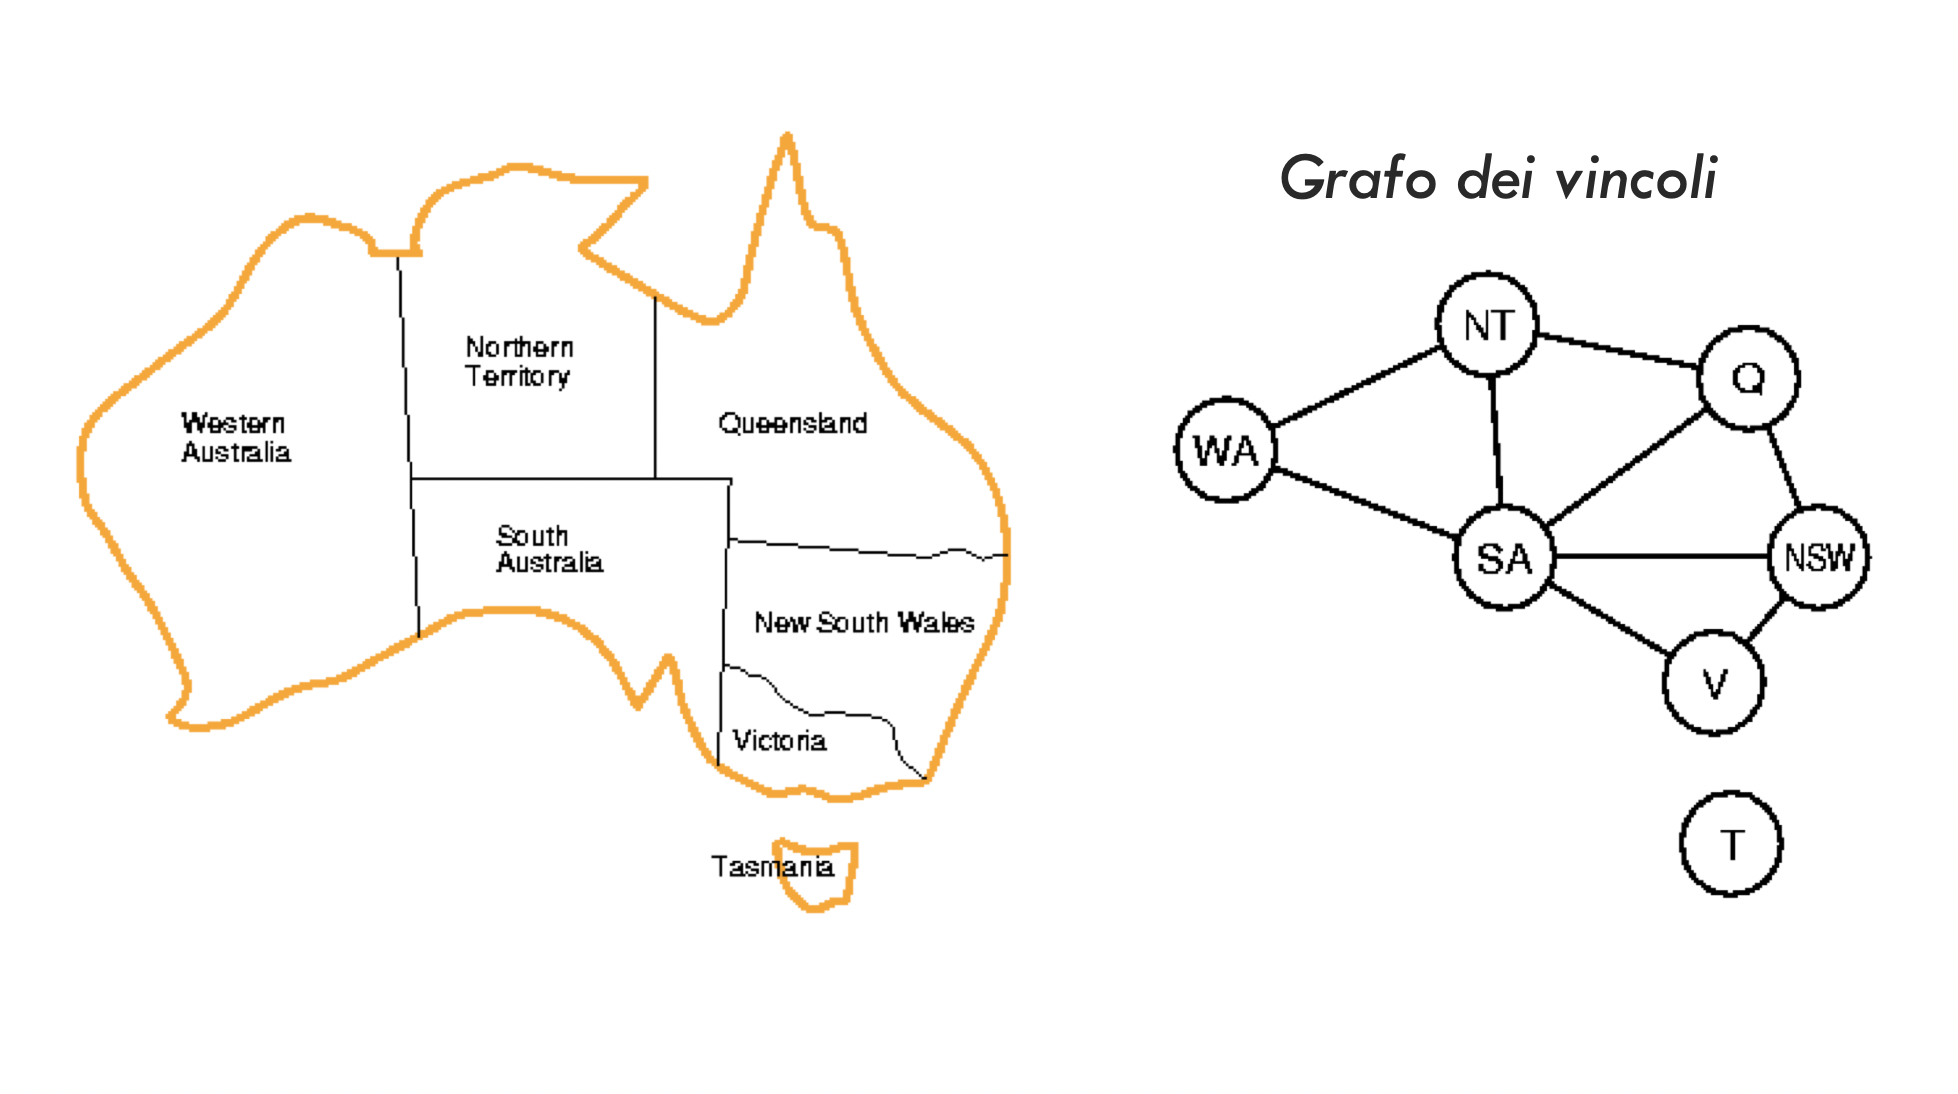
\includegraphics[scale=0.35]{Images/mappacolorata.png}
\end{figure}
Problema: Si tratta di colorare i diversi paesi sulla mappa con tre colori in modo che paesi adiacenti abbiano colori diversi.
\begin{enumerate}
    \item X = \{WA, NT, SA, Q, NSW, V, T\}
    \item $D_{WA} = D_{NT} = D_{SA} = D_Q = D_{NSW} = D_{V} = D_T$ = \{red, green, blue\}
    \item C = \{$WA \neq NT, WA \neq SA, NT \neq Q, NT \neq SA, SA \neq Q, SA \neq NSW, SA \neq V, NSW \neq V, NSW \neq Q$\}
\end{enumerate}

\subsubsection{Problema 8 regine}
Problema: Si tratta di posizionare le 8 regine sulla scacchiera senza che nessuna sia in grado di mangiarne un'altra.
\begin{enumerate}
    \item X = \{$Q_1, ..., Q_8$\} \quad una regina per colonna della scacchiera
    \item $D_i$ = \{1,2,3,4,5,6,7,8\} \quad numero di riga
    \item C = vincoli di non attacco
\end{enumerate}

\subsection{Strategie per problemi CSP}
Fin'ora potevamo solo ricercare la soluzione nel grafo degli stati, invece adesso possiamo usare delle euristiche specializzate per questa classe di problemi. Possiamo fare delle inferenze che ci portano a restringere i domini e quindi a limitare la ricerca, in più possiamo eseguire backtracking intelligente.

\subsection{Ricerca per problemi CSP}
Ad ogni passo si assegna una variabile, la massima profondità della ricerca è fissata dal numero di variabili n. L’ampiezza dello spazio di ricerca invece è definito da $|D_1| * |D_2| * ... * |D_n|$ (dove $|D_i|$ é il numero di elementi del dominio di $X_i$). Il fattore di diramazione è pari a $n*d$ al primo passo cioè posso scegliere tra d valori da assegnare a n variabili, al secondo passo $(n-1)*d$ e così via... si genera così un albero con $n! * d^n$ foglie anche se esistono al massimo $d^n$ assegnamenti completi differenti. Possiamo ridurre drasticamente lo spazio di ricerca sfruttando il fatto che il goal-test è commutativo (non è importante l’ordine con cui scelgo le variabili, quindi ad ogni livello posso scegliere una sola variabile a cui assegnare un valore). Con questa restrizione otteniamo $d^n$ foglie come volevamo.

\subsection{Ricerca con backtracking (BT) a profondità limitata}
Si esegue un controllo anticipato sulla violazione dei vincoli, perché è inutile andare avanti fino alla fine e poi controllare la correttezza. La ricerca è limitata in profondità dal numero di variabili quindi il metodo è completo. L'algoritmo sceglie ripetutamente una variabile senza assegnamento e a turno prova tutti i valori del dominio di quella variabile fino a trovare una soluzione. Se viene trovata una inconsistenza l'algoritmo si ferma ed esegue il backtracking facendo provare alle chiamate precedenti un nuovo valore.
\begin{figure}[H]
\centering
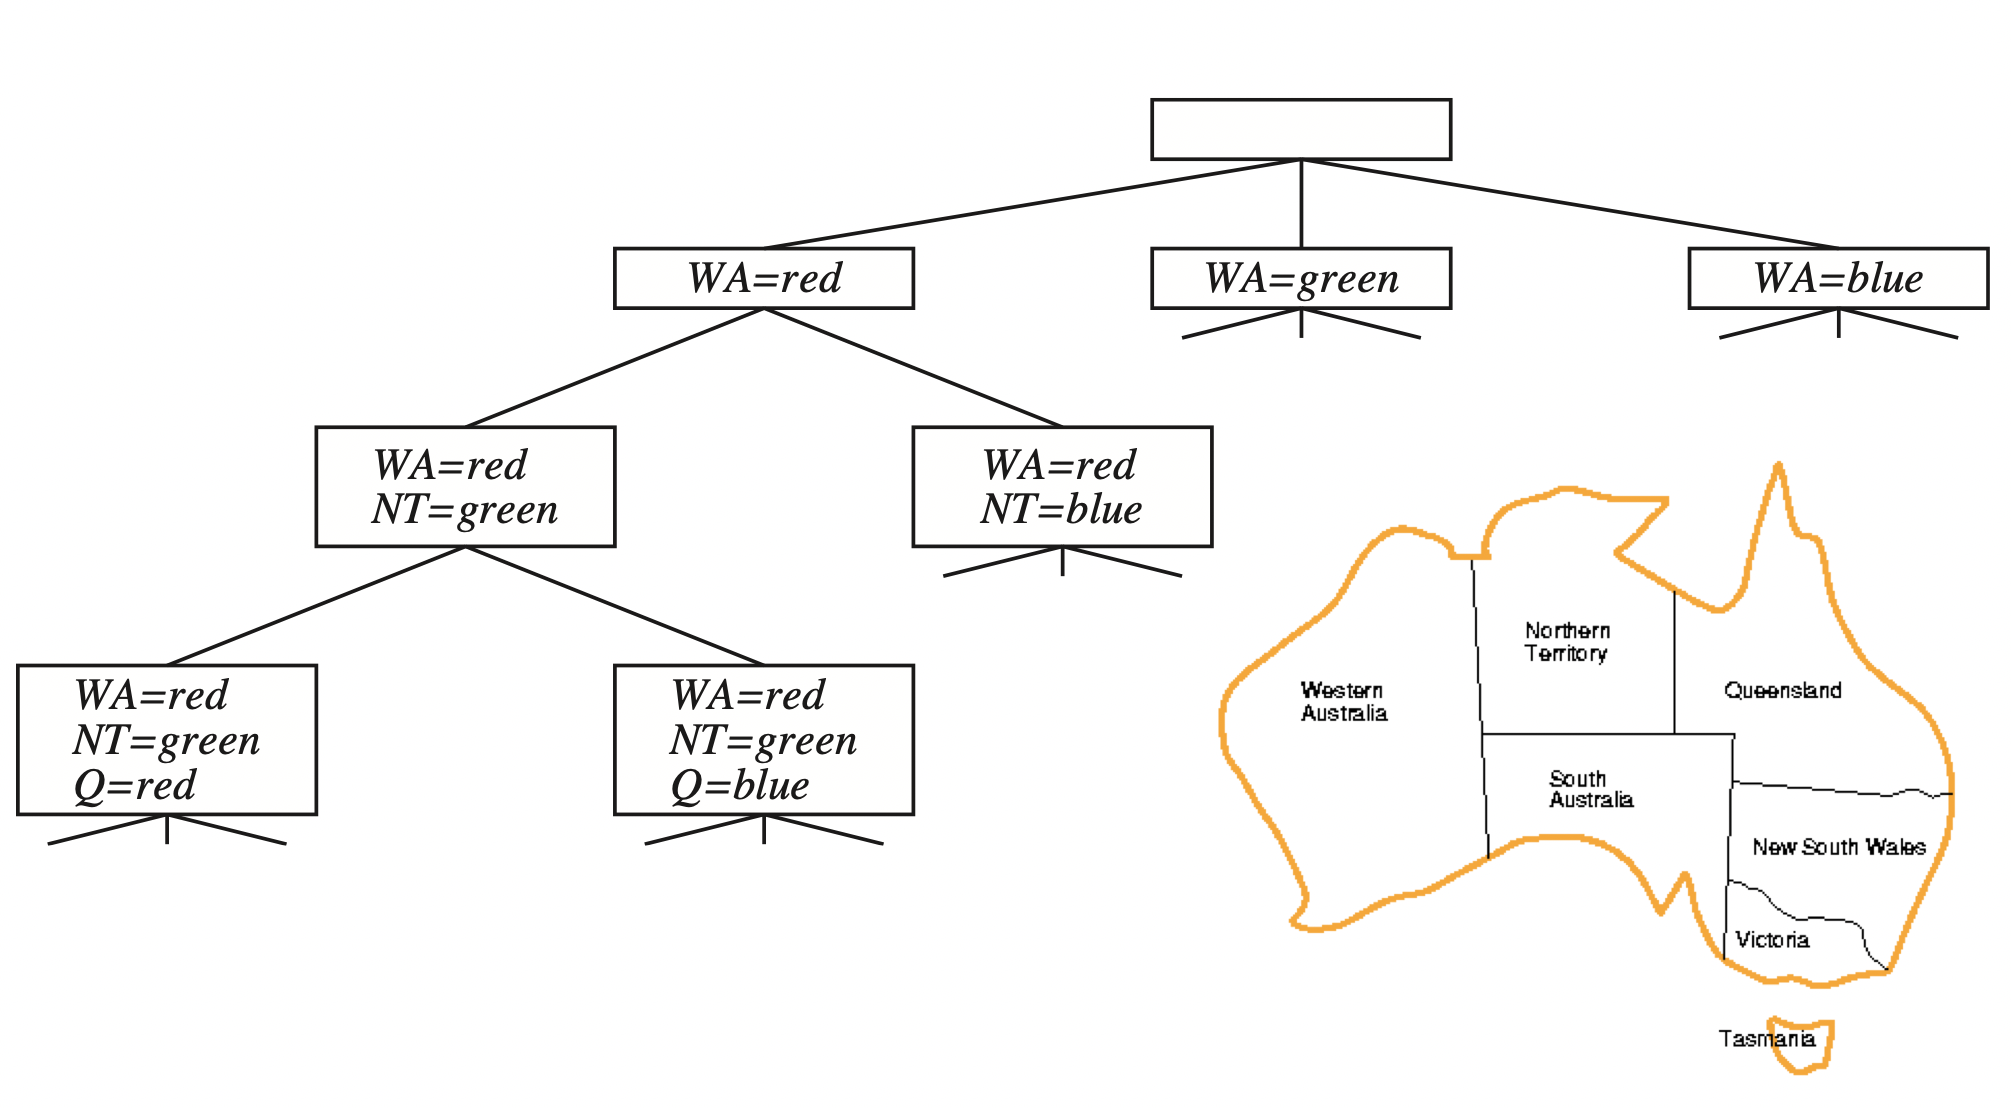
\includegraphics[scale=0.35]{Images/mappacoloratabacktracking.png}
\end{figure}

\subsection{Codice Algoritmo backtracking}
\begin{figure}[H]
\centering
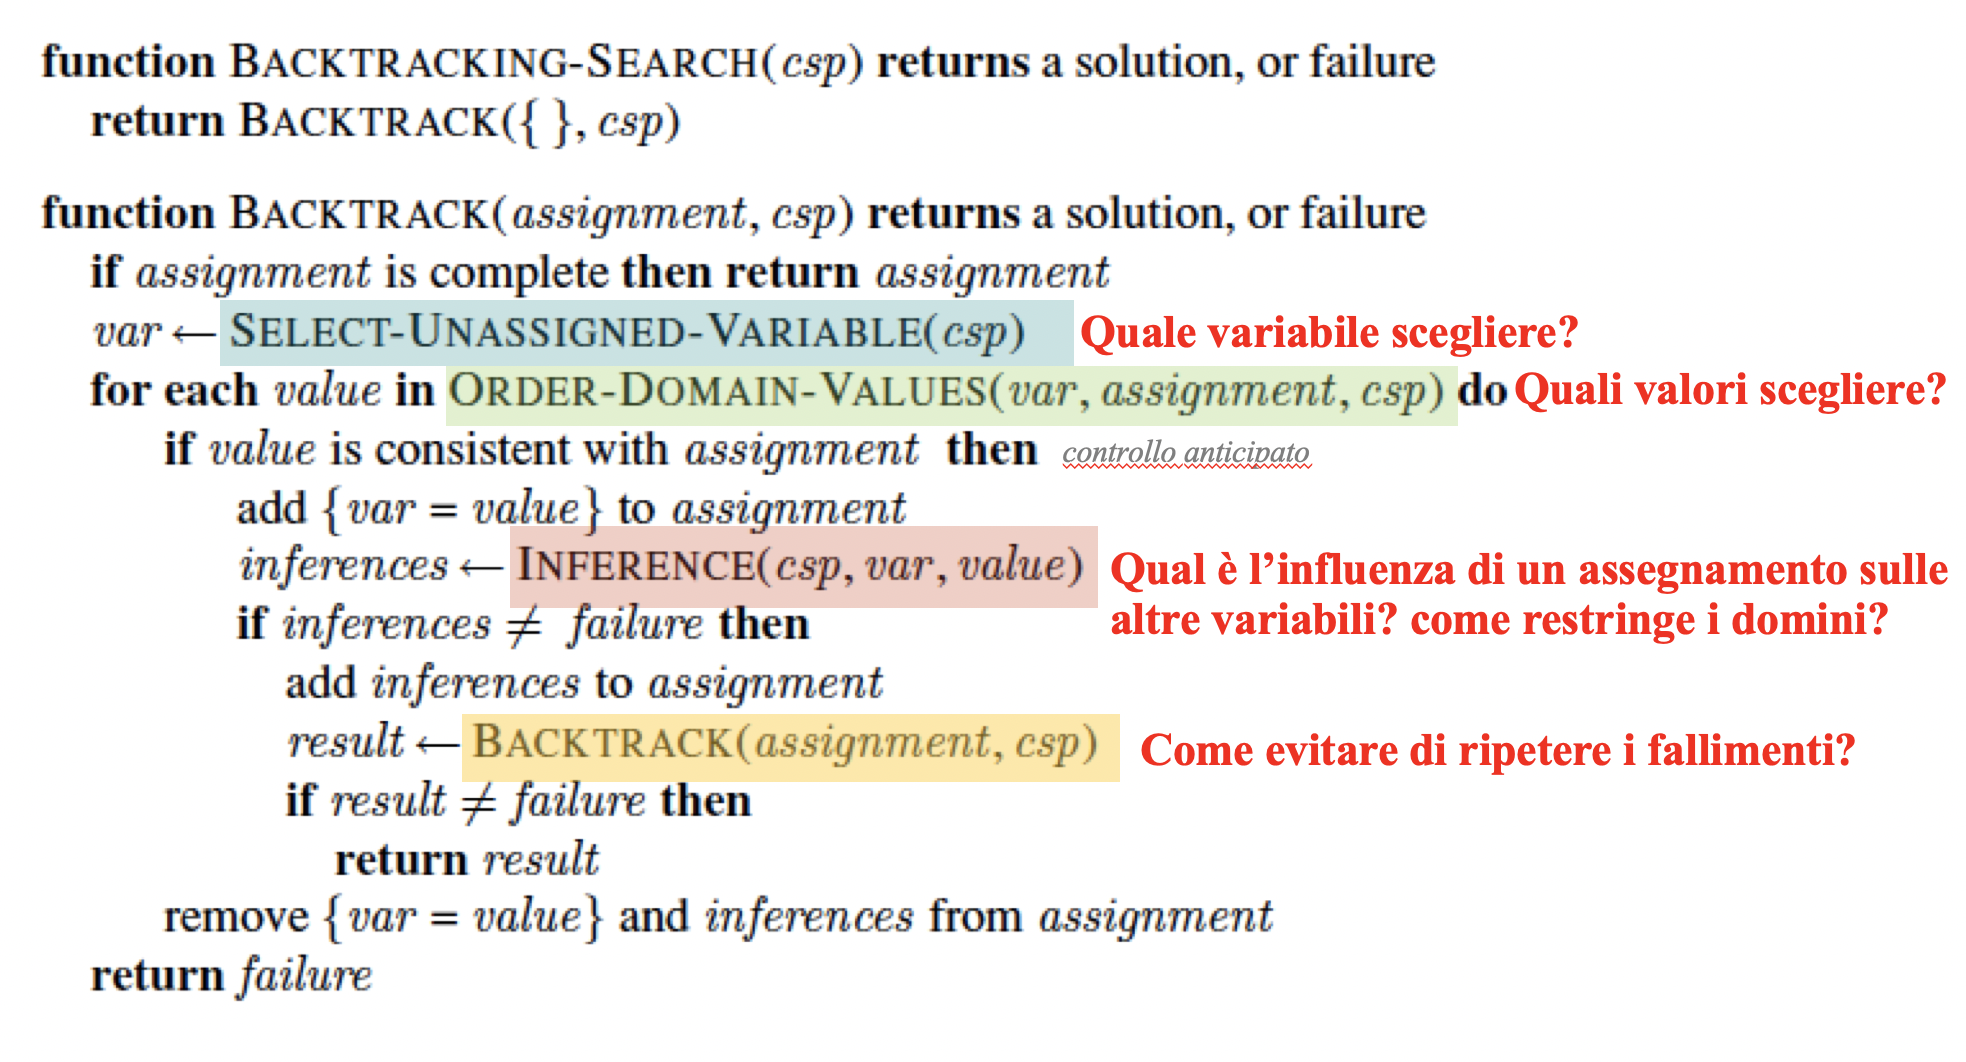
\includegraphics[scale=0.4]{Images/algoritmobacktracking.png}
\end{figure}
\textcolor{red}{Le parti evidenziate sono i punti dove posso usare euristiche!}
\subsubsection{Select-Unassigned-Variable()}
Scelta delle variabili: qual é la prossima variabile da scegliere?
\begin{itemize}
    \item MRV (Minimum Remaining Values): scegliere la variabile che ha meno valori legali (residui) da poter assegnare, cioè la variabile più vincolata. Si scoprono prima i fallimenti (fail first)!
    \item Euristica del grado: scegliere la variabile coinvolta in più vincoli con le altre variabili (la variabile più vincolante o di grado maggiore). (Usata a parità di MRV)
\end{itemize}

\subsubsection{Order-Domain-Values()}
Scelta dei valori: una volta scelta la variabile, come scegliere il valore da assegnare?
\begin{itemize}
    \item Valore meno vincolante: scegliamo il valore che esclude meno valori per le altre variabili direttamente collegate alla variabile scelta. Meglio valutare prima un assegnamento che ha più probabilità di successo, se volessimo tutte le soluzioni l’ordine non sarebbe importante.
\end{itemize}

\subsubsection{Inference()}
Propagazione di vincoli: qual è l'influenza di un assegnamento sulle altre variabili?
\begin{itemize}
    \item Verifica in avanti (Forward Checking o FC): assegnato un valore ad una variabile, si possono eliminare i valori incompatibili per le altre variabili direttamente collegate da vincoli.
    \item Consistenza di nodo e arco: si restringono i valori dei domini delle variabili tenendo conto dei vincoli unari e binari su tutto il grafo (se una variabile ad un certo punto ha il dominio ridotto all'insieme vuoto, si esegue immediatamente backtracking. Altrimenti si itera finché tutti i nodi ed archi sono consistenti).
\end{itemize}

\subsubsection{Backtrack()}
Quando la ricerca arriva ad un assegnamento che viola i vincoli, come posso evitare di ripetere in futuro lo stesso errore?
\begin{itemize}
    \item Backtracking Cronologico: viene cambiato il valore dell'ultima variabile assegnata, continuando a fallire fino al soddisfacimento dei vincoli.
    \item Backtracking Intelligente: si considerano alternative solo per le variabili che hanno causato il fallimento ($X_i, X_j, ...$), cioè un "insieme dei conflitti". Ad esempio, nel problema delle regine, si parte con tutte le variabili assegnate (tutte le regine sulla scacchiera) e ad ogni passo si modifica l’assegnamento ad una variabile per cui un vincolo è violato (si muove una regina minacciata su una colonna). Questo è un algoritmo di riparazione euristica. Un’altra euristica potrebbe consistere nello scegliere un nuovo valore che crea meno conflitti (euristica dei conflitti minimi).
\end{itemize}
\clearpage 

%Lezione 7
\section{Agenti Logici KB}
Vogliamo migliorare le capacità razionali dei nostri agenti dotandoli di rappresentazioni di mondi più complessi. Il mondo é tipicamente complesso, ci serve una rappresentazione parziale e incompleta (una astrazione) del mondo, utile agli scopi dell'agente. Per descrivere ambienti parzialmente osservabili e complessi ci servono linguaggi di rappresentazione della conoscenza più espressivi, ma soprattutto con capacità inferenziali. Gli agenti basati su conoscenza sono dotati di una KB (knowledge base) con conoscenza espressa in maniera esplicita e dichiarativa. La conoscenza può essere codificata a mano, ma anche estratta dai testi o appresa dall'esperienza.

\subsection{Approccio dichiarativo VS Approccio procedurale}
L'approccio dichiarativo consiste nella creazione di una KB che racchiude tutta la conoscenza necessaria a decidere l’azione da compiere in forma dichiarativa. L’alternativa (approccio procedurale) è scrivere un programma che implementa il processo decisionale, una volta per tutte. \newline
Un agente KB è più flessibile: più semplice acquisire conoscenza in modo incrementale e modificare il comportamento con l’esperienza!

\subsection{Tell-Ask} 
Un agente basato su conoscenza mantiene una base di conoscenza (KB), cioè un insieme di enunciati espressi in un linguaggio di rappresentazione. L'agente interagisce con la KB mediante una interfaccia funzionale definita come Tell-Ask:
\begin{itemize}
    \item Tell: per aggiungere nuovi enunciati a KB
    \item Ask: per interrogare la KB
    \item Retract: per eliminare enunciati
\end{itemize}
Gli enunciati nella KB rappresentano le credenze dell'agente, le risposte X dell'agente quindi devono essere tali che X è una conseguenza (discende necessariamente) della KB. \newline 
Il nostro obiettivo sarà capire quando, avendo una base di conoscenza KB contenente una rappresentazione dei fatti che si ritengono veri, un certo fatto $\alpha$ è vero di conseguenza ($KB \models \alpha$, cioè $\alpha$ è conseguenza logica della KB).

\subsection{Base di conoscenza o Base di dati?}
Qual è la differenza tra una KB e un database?
\begin{itemize}
    \item Base di conoscenza: una rappresentazione esplicita dello stato, parziale e compatta, espressa in un linguaggio simbolico, che contiene fatti di tipo specifico e fatti di tipo generale o anche regole. Quello che caratterizza una base di conoscenza è la capacità inferenziale, cioè la capacità di derivare nuovi fatti da quelli memorizzati esplicitamente. 
    \item Base di dati: solo fatti specifici e posso solo interrogarla, non ho modo di inferire nuovi fatti.
\end{itemize}
Ma il problema fondamentale della rappresentazione della conoscenza sta nel trovare il giusto compromesso tra: espressività del linguaggio di rappresentazione e complessità del meccanismo inferenziale. Sfortunatamente più il linguaggio è espressivo, meno  efficiente è il meccanismo inferenziale.

\subsection{Formalismi per la rappresentazione della conoscenza}
Un formalismo per la rappresentazione della conoscenza ha tre componenti:
\begin{enumerate}
    \item Una sintassi: cioè un linguaggio composto da un vocabolario e regole per la formazione delle frasi (enunciati).
    \item Una semantica: stabilisce una corrispondenza tra gli enunciati e fatti del mondo. Se un agente ha un enunciato X nella sua KB, crede che il fatto corrispondente sia vero nel mondo.
    \item Un meccanismo inferenziale: (codificato o meno tramite regole di inferenza come nella logica) che ci consente di inferire nuovi fatti. 
\end{enumerate}
A questo punto, qual è la complessità computazionale di sapere se $\alpha$ è conseguenza logica della KB nei vari linguaggi logici? Quali sono gli algoritmi di decisione e le strategie di ottimizzazione? I linguaggi logici, calcolo proposizionale (PROP) e logica dei predicati (FOL), sono adatti per la rappresentazione della conoscenza?

\section{Agenti Logici: Calcolo proposizionale}

\subsection{Sintassi (regole)}
La sintassi definisce quali sono le frasi legittime (ben formate) del linguaggio.
\begin{itemize}
    \item simbolo $\to$ P | Q | R ...
    \item formula $\to$ formulaAtomica | formulaComplessa
    \item formulaAtomica $\to$ Ture | False | simbolo
    \item formulaComplessa $\to \neg$ formula | formula $\land$ formula | formula $\lor$ formula | formula $\Rightarrow$ formula | formula $\Leftrightarrow$ formula
\end{itemize}
Possiamo omettere le parentesi assumendo questa precedenza tra gli operatori:
\begin{quote}
    $\neg  >  \land  >  \lor  >  \Rightarrow, \Leftrightarrow$
\end{quote}

\subsection{Semantica (significato)}
La semantica definisce il significato di un enunciato, cioè se esso è vero o falso rispetto ad una interpretazione. Una interpretazione definisce un valore di verità per tutti i simboli proposizionali. Il significato di una frase è determinato dal significato dei suoi componenti, a partire dai simboli proposizionali.

\subsection{Conseguenza logica}
Come abbiamo visto precedentemente, il problema è capire quando, data una base di conoscenza KB contenente una rappresentazione dei fatti che si ritengono veri, un certo fatto $\alpha$ è vero di conseguenza. (KB $\models \alpha$, cioè $\alpha$ è conseguenza logica della KB). \newline
Una formula $\alpha$ è conseguenza logica di un insieme di formule KB se e solo se in ogni modello\footnote{Modello: un'attribuzione di un significato a tutti gli enunciati (le formule) del linguaggio che le rende tutte vere} di KB anche $\alpha$ è vera. \newline
Indicheremo con M($\alpha$) i modelli di $\alpha$, cioè l’insieme delle interpretazioni che rendono $\alpha$ vera, e con M(KB) i modelli dell'insieme di formule in KB otteniamo:
\begin{quote}
    KB $\models \alpha \Leftrightarrow$ M(KB) $\subseteq$ M($\alpha$)
\end{quote}

\subsection{Il mondo del Wumpus}
Il mondo del Wumpus è una caverna fatta di stanze connesse tra di loro. Il Wumpus mangia chiunque entri nella stanza in cui si trova. Il Wumpus può essere ucciso dall’agente, che ha solo una freccia a disposizione. In alcune stanze sono presenti dei pozzi: se l'agente entra in una di queste stanze cade nel pozzo e muore. In una delle stanze si trova l’oro e l’obiettivo dell'agente è di trovarlo e tornare a casa sano e salvo. L’agente non conosce l’ambiente, né la sua locazione. Solo all'inizio sa dove si trova (in [1,1]). In questo problema gli ambienti sono generati a caso e alcuni di questi non sono risolubili (ma sappiamo che lo stato (1,1) è safe): l’agente in alcune situazioni deve decidere se rischiare di essere ucciso pur di trovare l’oro e quando conviene tornare a casa a mani vuote.
\begin{figure}[H]
\centering
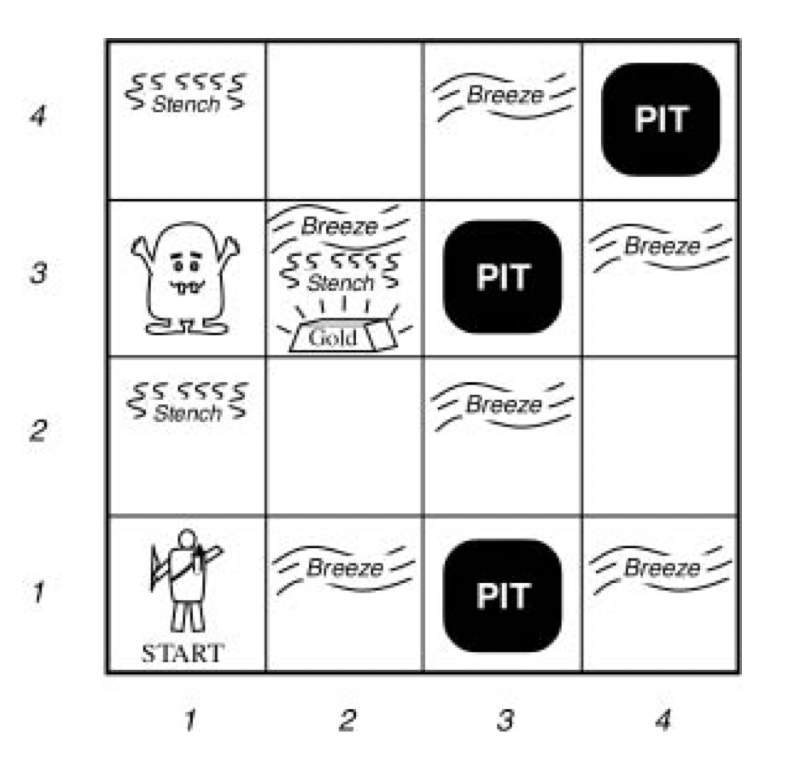
\includegraphics[scale=0.4]{Images/wumpus_a.png}
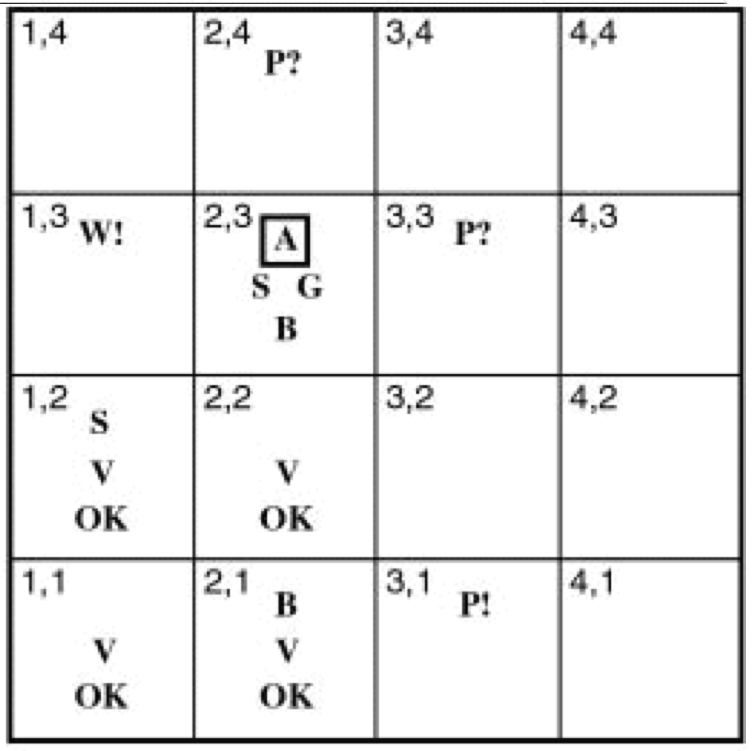
\includegraphics[scale=0.4]{Images/wumpus_b.png}
\caption{Wumpus' world}
\end{figure}
\begin{itemize}
    \item Misura delle prestazioni:
    \begin{itemize}
        \item +1000 se trova l’oro, torna in [1,1] e esce
        \item -1000 se muore
        \item -1 per ogni azione
        \item -10 se usa la freccia
    \end{itemize}
    \item Percezioni:
    \begin{itemize}
        \item \textbf{puzzo} nelle caselle adiacenti al Wumpus
        \item \textbf{brezza} nelle caselle adiacenti alle buche
        \item \textbf{luccichio} nelle caselle con l‘oro
        \item \textbf{bump} se sbatte in un muro
        \item \textbf{urlo} se il Wumpus viene ucciso
        \item L’agente non percepisce la sua locazione
    \end{itemize}
    \item Azioni:
    \begin{itemize}
        \item avanti
        \item destra
        \item sinistra
        \item afferra oggetto
        \item scaglia la freccia
        \item esci
    \end{itemize}
\end{itemize}
Le percezioni sono una quintupla [puzzo, brezza, luccichio, bump, urlo]. ([none, none, none, none, none] se non percepisce niente).
\subsubsection{Esempio dal mondo del Wumpus}
KB = \{$B_{2,1}, \neg B_{1,1} , +$ le regole del WumpusWorld\} \newline 
Vogliamo stabilire l’assenza di pozzi in [1,2] e in [2,2] \newline
KB $\models \neg P_{1,2}$? \newline
KB $\models \neg P_{2,2}$? \newline
Ci sono otto possibili interpretazioni o mondi, considerando solo l’esistenza di pozzi nelle 3 caselle $P_{1,2} \quad P_{2,2} \quad P_{3,1}$ (perchè non posso muovermi in diagonale). Guardando le immagini sottostanti, a sinistra prendiamo tutti i mondi in cui non c'è pozzo in [1,2] e notiamo che facendo così includo tutti i mondi della mia KB, quindi KB $\vdash \neg P_{1,2}$. A destra prendo i mondi dove non c'è pozzo in [2,2] e vediamo che questi non includono tutti i mondi della mia KB, quindi KB $\nvDash \neg P_{2,2}$ .
\begin{figure}[H]
\centering
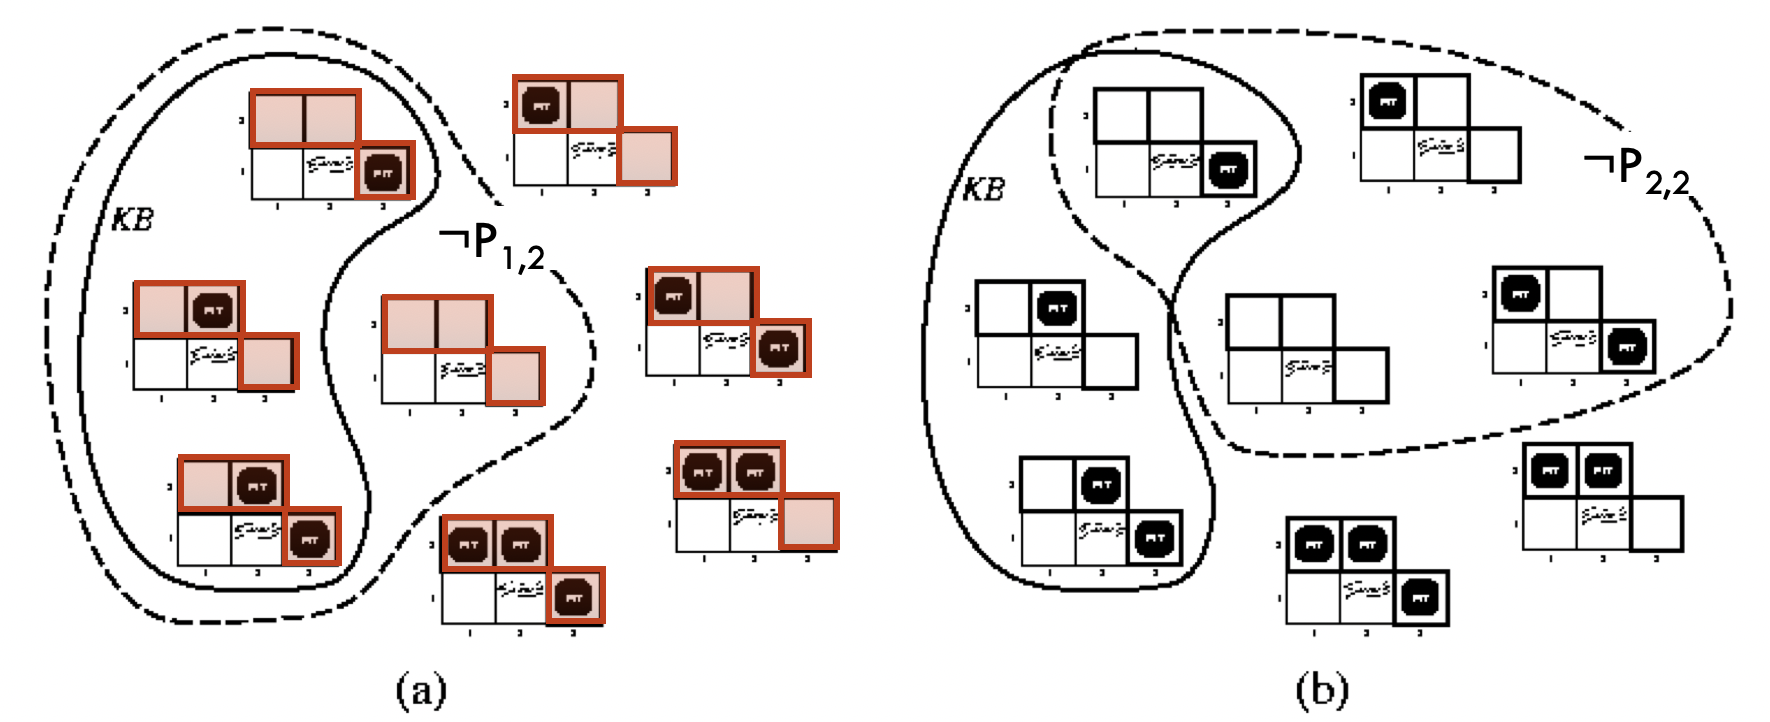
\includegraphics[scale=0.45]{Images/wumpusconslogica.png}
\end{figure}

\subsection{Formule logiche, Validità e Soddisfacibilità}
\begin{figure}[H]
\centering
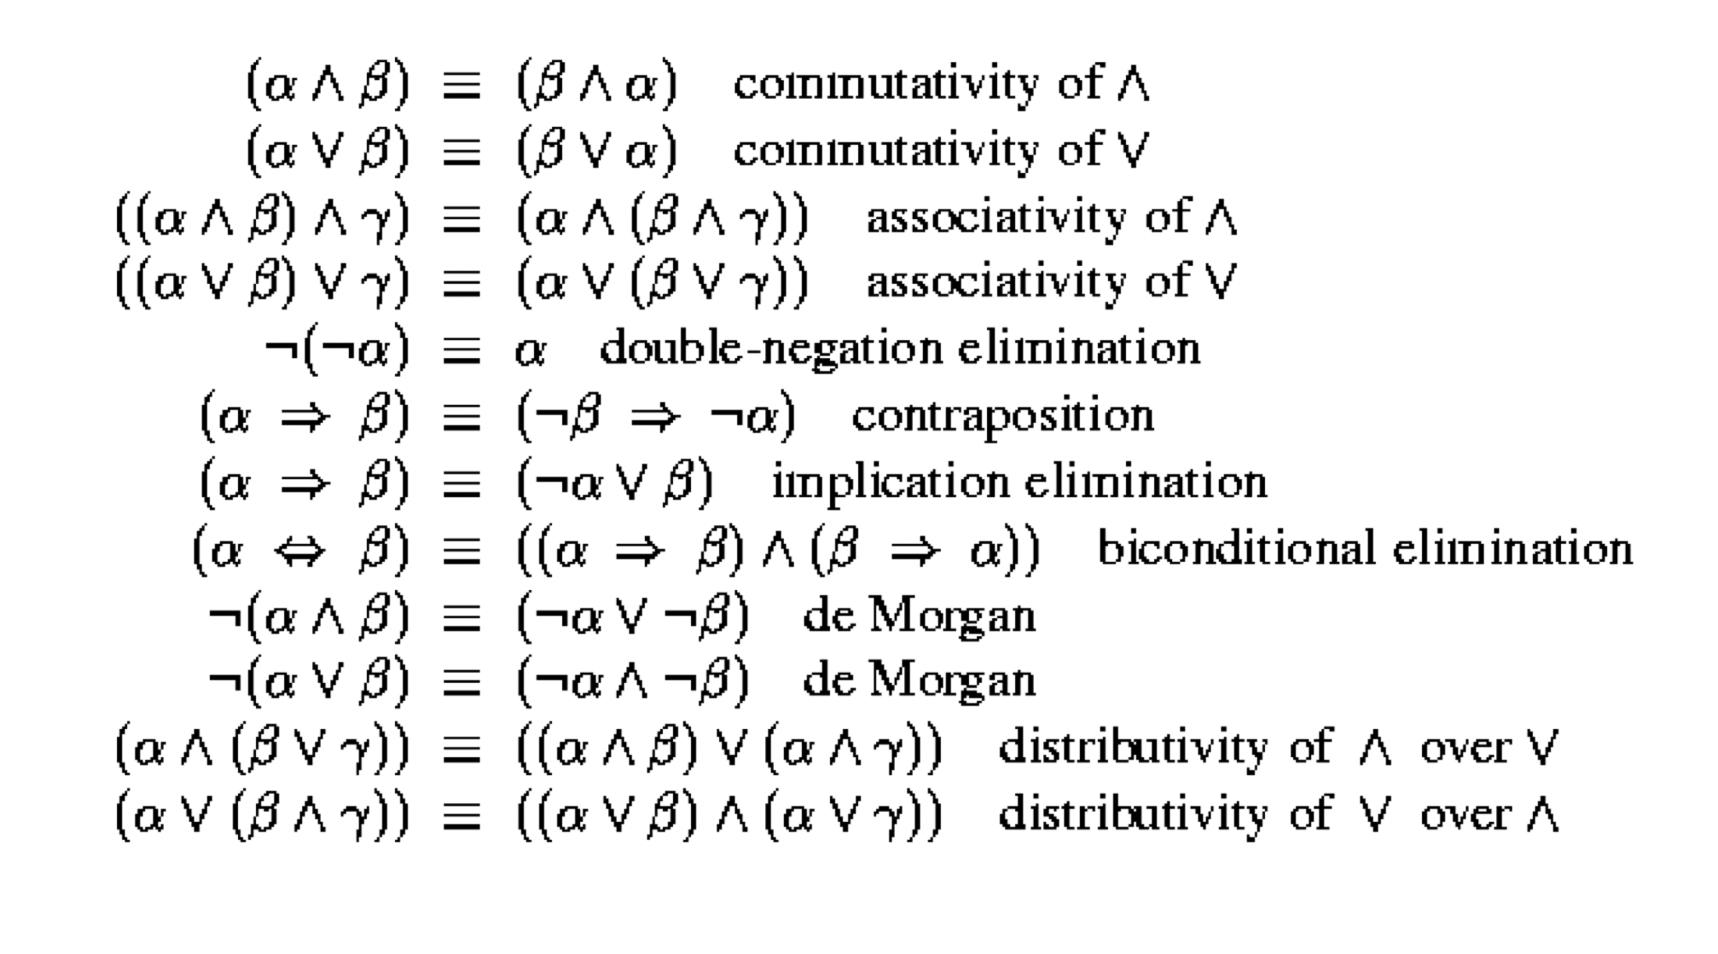
\includegraphics[scale=0.35]{Images/formulelogiche.png}
\caption{Equivalenze Logiche (leggi)}
\end{figure}
A valida sse è vera in tutte le interpretazioni (detta anche tautologia). \newline
A soddisfacibile sse esiste una interpretazione in cui A è vera. \newline
A è valida sse $\neg A$ è insoddisfacibile.

\subsection{Inferenza per calcolo proposizionale (PROP)}
\begin{itemize}
    \item Model checking: una forma di inferenza che fa riferimento alla definizione di conseguenza logica (si enumerano i possibili modelli e si controllano tramite le tabelle di verità)
    \item Algoritmi per la soddisfacibilità: problemi riconducibili ad altri problemi. \newline KB $\models$ A sse $KB\land \neg A$ è insoddisfacibile.
\end{itemize}

\subsection{Algoritmo TT-Entails (Model Checking)}
Come facciamo a sapere se KB $\models \alpha$? L'algoritmo TT-Entails enumera tutte le possibili interpretazioni di KB (k simboli, $2^k$ possibili interpretazioni). Per ciascuna interpretazione: 
\begin{itemize}
    \item Se non soddisfa KB $\to$ OK (non ci interessa, andiamo avanti)
    \item Se soddisfa KB $\to$ si controlla che soddisfi anche $\alpha$. \newline 
    Se si trova anche solo una interpretazione che soddisfa KB e non $\alpha$ la risposta è NO.
\end{itemize} 

\subsubsection{Esempio TT-Entails}
\begin{figure}[H]
\centering
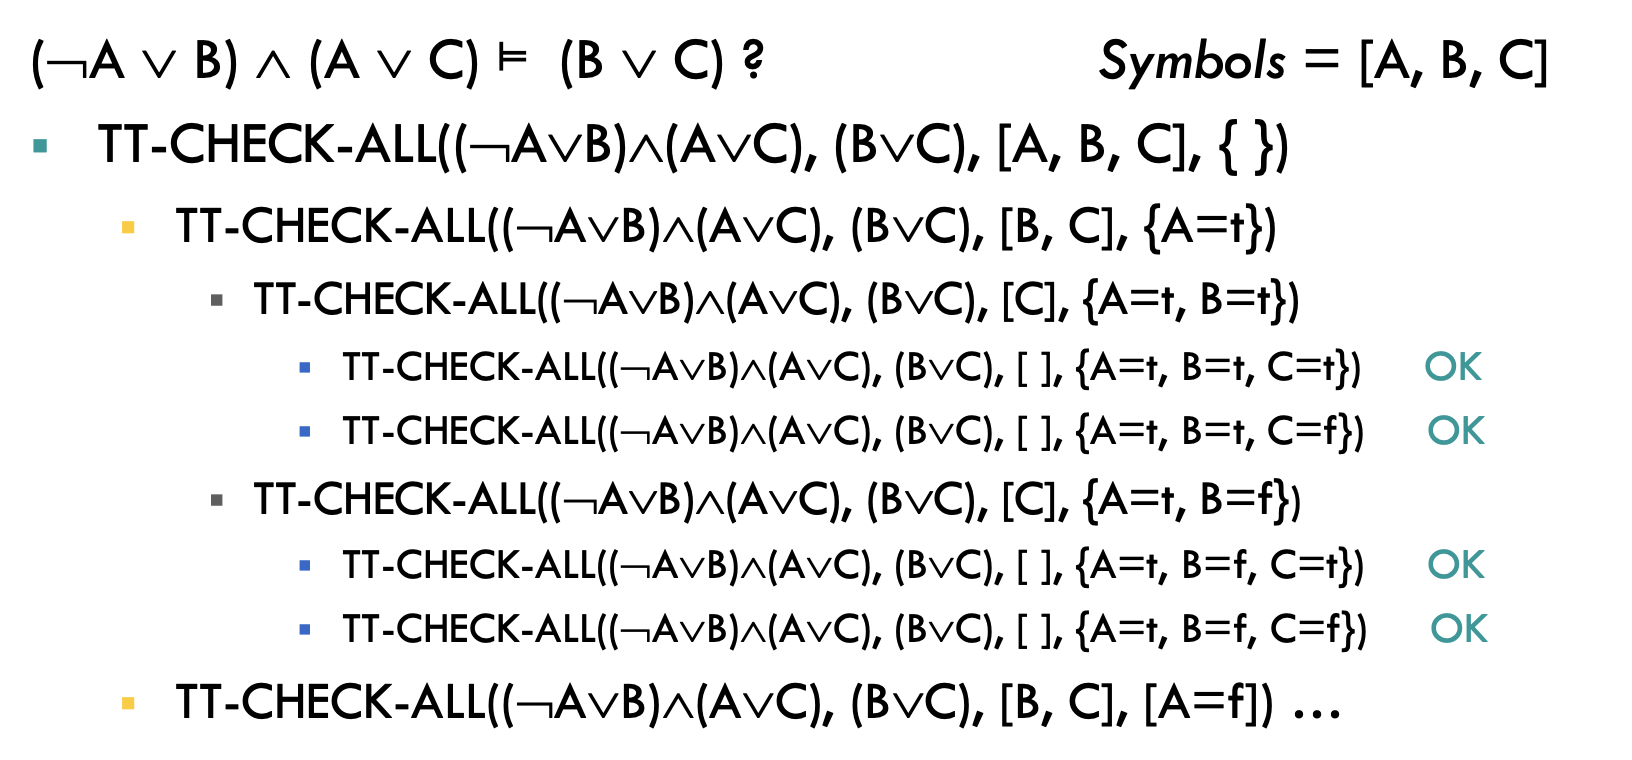
\includegraphics[scale=0.37]{Images/ttentailscheck.png}
\end{figure}
Solo alla fine, dopo avere provato tutti i possibili assegnamenti, possiamo rispondere se Vero o Falso.

\subsection{Algoritmo DPLL (Alg. Soddisfacibilità)}
\subsubsection{Forma a clausole}
Gli algoritmi per la soddisfacibilità usano KB in forma a clausole. \newline 
Ad esempio \{A, B\} \{$\neg$B, C, D\} \{$\neg$A, F\} è una forma normale congiuntiva cioè una congiunzione di disgiunzioni letterali. Il suo significato quindi è: \newline 
(A $\lor$ B) $\land$ ($\neg$ B $\lor$ C $\lor$ D) $\land$ ($\neg$ A $\lor$ F), la cosa interessante è che non è restrittiva: è sempre possibile ottenerla con trasformazioni che preservano l’equivalenza logica. \newline 
I passi da seguire per ottenere la forma a clausole sono: 
\begin{enumerate}
    \item Eliminazione della $\Leftrightarrow$: (A $\Leftrightarrow$ B) $\equiv$ (A $\Rightarrow$ B) $\land$ (B $\Rightarrow$ A)
    \item Eliminazione dell’ $\Rightarrow: (A \Rightarrow B) \equiv (\neg A \lor B)$
    \item Negazioni all’interno: \begin{itemize}
        \item $\neg (A \lor B) \equiv (\neg A \land \neg B)$	(de Morgan)	
        \item $\neg (A \land B) \equiv (\neg A \lor \neg B)$
    \end{itemize}   
    \item Distribuzione di $\lor$ su $\land$: $(A \lor (B \land C)) \equiv (A \lor B) \land (A \lor C)$
\end{enumerate}
L'algoritmo DPLL sfrutta la soddisfacibilità di $KB \models A$ se $KB \land \neg A$ = \{\}. Parte da una KB in forma a clausole, avviene una enumerazione in profondità di tutte le possibili interpretazioni alla ricerca di un modello. Tre miglioramenti rispetto a TT-Entails: 
\begin{enumerate}
    \item Terminazione anticipata: Si può decidere sulla verità di una clausola anche con interpretazioni parziali, basta che un letterale sia vero. Ad esempio se A è vero lo sono anche \{A, B\} e \{A, C\} indipendentemente dai valori di B e C. (ricordiamo che sono in $\lor$!). Se anche una sola clausola è falsa l'interpretazione non può essere un modello dell'insieme di clausole. 
    \item Simboli puri: un simbolo puro è un simbolo che appare con lo stesso segno in tutte le clausole. Ad esempio \{$A, \neg B\} \{ \neg B, \neg C\} \{C, A\}$ dove A e B sono puri. Nel determinare se un simbolo è puro se ne possono trascurare le occorrenze in clausole già rese vere cioè i simboli puri possono essere assegnati a True se il letterale è positivo, False se negativo. Facendo così non si eliminano modelli utili, se le clausole hanno un modello continuano ad averlo dopo questo assegnamento. L’assegnamento è obbligato.
    \item Clausole unitarie: una clausola con un solo letterale non assegnato, ad esempio \{B\} è unitaria ma anche \{B, $\neg$C\} è unitaria quando C = True. Conviene assegnare prima valori al letterale in clausole unitarie. L'assegnamento è univoco (True se positivo, False se negativo).
\end{enumerate}

\subsubsection{Esempio DPLL}
KB = ($\{\neg B_{1,1}, P_{1,2}, P_{2,1}\} \{\neg P_{1,2}, B_{1,1}\} \{\neg P_{2,1}, B_{1,1}\} \{\neg B_{1,1}\}) \models \{\neg P_{1,2} \}$? \newline
Aggiungiamo \{$P_{1,2}$\} (perché sarebbe $\neg (\neg P_{1,2})$) e vediamo se l’insieme è insoddisfacibile: \newline 
DPLL($\{\neg B_{1,1}, P_{1,2}, P_{2,1}\} \{\neg P_{1,2}, B_{1,1}\} \{\neg P_{2,1}, B_{1,1}\} \{\neg B_{1,1}\} \{P_{1,2} \}$) \newline
Notiamo che \{$P_{1,2}$ \} è unitaria quindi assegnamo $P_{1,2}$=True. \newline
La prima clausola $\{\neg B_{1,1}, P_{1,2}, P_{2,1}\}$ e  $\{P_{1,2} \}$ sono soddisfatte. \newline
La seconda clausola $\{\neg P_{1,2}, B_{1,1}\}$ diventa unitaria, $B_{1,1}$=True. \newline A questo punto $\{\neg P_{1,2}, B_{1,1}\}$ e $\{\neg P_{2,1}, B_{1,1}\}$ sono soddisfatte, ma $\{\neg B_{1,1}\}$ no (perché prima abbiamo assegnato $B_{1,1}$=True, quindi $\neg B_{1,1}$=False). \newline FAIL! \newline 
Non esistono modelli, quindi possiami dire che $\neg P_{1,2}$ è conseguenza logica della KB.

\subsubsection{Miglioramenti DPLL}
DPLL è completo e termina sempre. Alcuni miglioramenti: analisi di componenti (se le variabili possono essere suddivise in sotto-insiemi disgiunti, cioè senza simboli in comune), ordinamento di variabili e valori (scegliere la variabile che compare in più clausole), backtracking intelligente e altre ottimizzazioni...

\subsection{Algoritmo WALK-SAT}
E' un algoritmo di ricerca locale, l'obiettivo è un assegnamento che soddisfa tutte le clausole (un modello) partendo da un assegnamento casuale. Ad ogni passo si cambia il valore di una proposizione (flip). Gli stati sono valutati contando il numero di clausole non soddisfatte (meno sono meglio è). Ci sono molti minimi locali, per non incapparci serve introdurre perturbazioni casuali, come succedeva con Hill Climbing con riavvio casuale o Simulated Annealing. WALK-SAT è uno degli algoritmi più semplici ed efficaci. \clearpage
WALK-SAT ad ogni passo: 
\begin{itemize}
    \item Sceglie a caso una clausola non ancora soddisfatta
    \item Sceglie un simbolo da modificare (flip) scegliendo con probabilità p (di solito 0,5) tra una delle due: \begin{itemize}
        \item Passo casuale: un simbolo a caso
        \item Passo di ottimizzazione: sceglie quello che rende più clausole soddisfatte
    \end{itemize}
    \item Si arrende dopo un certo numero di flip predefinito (variabile max-flips)
\end{itemize}

\subsubsection{Esempio WALK-SAT}
Come euristica usiamo il numero di clausole soddisfatte (valore da massimizzare). \newline
\textcolor{red}{Rosso: passo casuale} \newline
\textcolor{blue}{Blu: passo di ottimizzazione} \newline
$(1)\{\neg B_{1,1}, P_{1,2}, P_{2,1}\}\quad (2)\{\neg P_{1,2}, B_{1,1}\}\quad (3)\{\neg P_{2,1}, B_{1,1}\} \quad (4)\{\neg B_{1,1}\}$ \newline
[$B_{1,1}=F, P_{1,2}=T, P_{2,1}=T$] \textcolor{red}{clausole 2, 3 F; scelgo clausola 2; a caso eseguo flip $B_{1,1}$} \newline
[$B_{1,1}=T, P_{1,2}=T, P_{2,1}=T$] \textcolor{blue}{clausola 4 F; scelgo 4; ottimizzazione: flip $B_{1,1}$ (unica scelta)}\newline
[$B_{1,1}=F, P_{1,2}=T, P_{2,1}=T$] \textcolor{red}{clausole 2, 3 F; scelgo clausola 2; a caso eseguo flip $P_{1,2}$}\newline
[$B_{1,1}=F, P_{1,2}=F, P_{2,1}=T$] \textcolor{blue}{clausola 3 F; scelgo 3; ottimizzazione: flip $P_{2,1}$}\newline
[$B_{1,1}=F, P_{1,2}=F, P_{2,1}=F$] modello

\subsubsection{Analisi WALK-SAT}
Se max-flips = $\infty$ e l’insieme di clausole è soddisfacibile prima o poi termina. Va bene per cercare un modello, sapendo che esiste, ma se è insoddisfacibile non termina. Non può essere usato per verificare l’insoddisfacibilità, il problema quindi è decidibile ma l’algoritmo non è completo.

\subsubsection{Problemi SAT difficili}
Se un problema ha molte soluzioni (problema sotto-vincolato) è più probabile che WALK-SAT ne trovi una in tempi brevi. Ma dato che SAT é un problema NP-Completo, alcune istanze richiedono tempo esponenziale per la risoluzione.
Un esempio è che nella seguente istanza esistono 16 soluzioni su 32 assegnamenti possibili, un assegnamento ha il 50\% di probabilità di essere giusto: in circa 2 passi random si indovina. \newline 
$(\neg D \lor \neg B \lor C) \land (B \lor \neg A \lor \neg C) \land (\neg C \lor \neg B \lor E) \land (E \lor \neg D \lor B) \land (B \lor E \lor \neg C)$ \newline quello che conta è il rapporto m/n, dove m è il numero di clausole (vincoli) e n il numero di simboli. In questo esempio 5/5=1, più è grande il rapporto, più vincolato è il problema.
\begin{figure}[H]
\centering
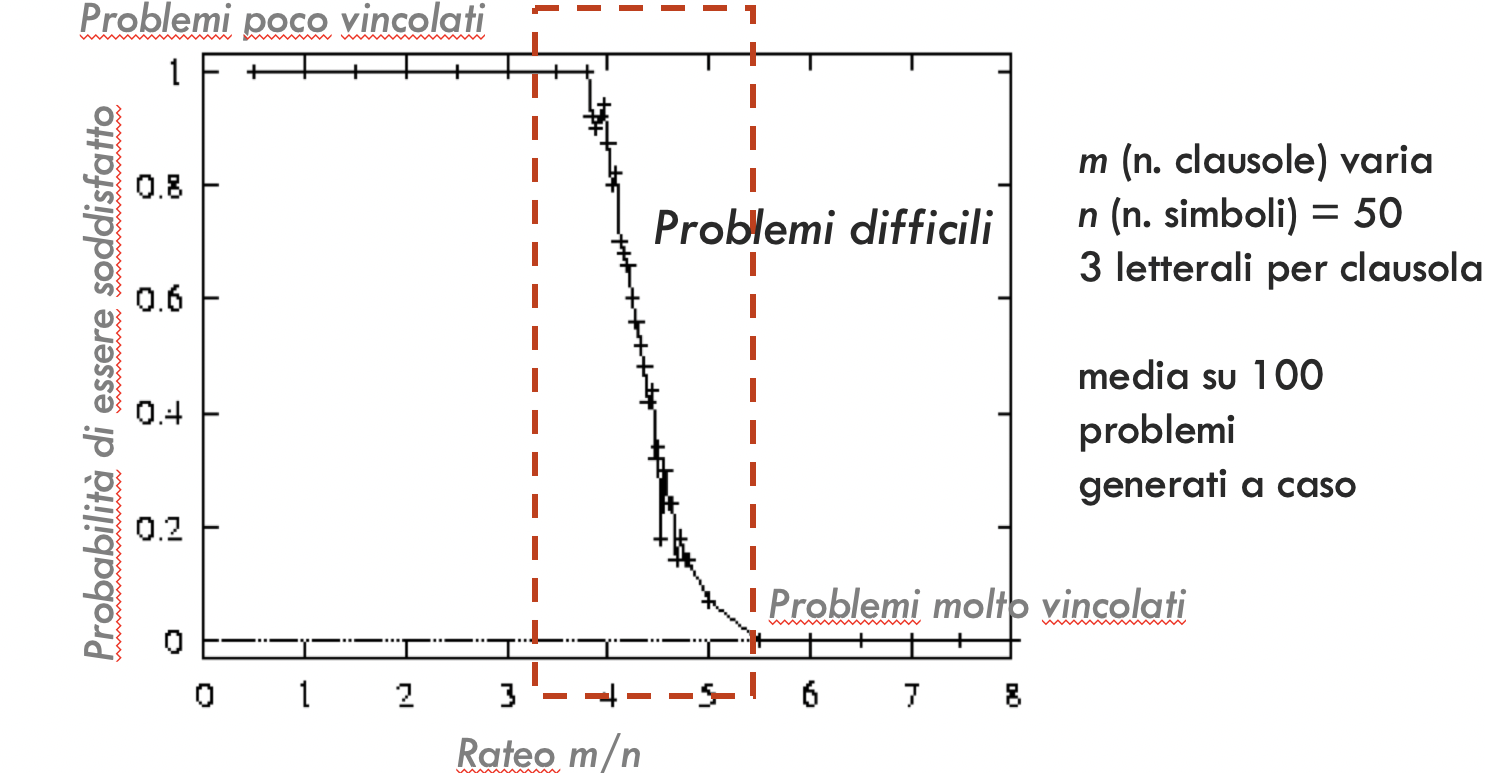
\includegraphics[scale=0.4]{Images/rateomn.png}
\end{figure}

\subsection{Inferenza come deduzione}
Un altro modo per decidere se KB $\models$ A è usare un meccanismo di deduzione, scriviamo KB $\vdash$ A  (A è deducibile da KB). La deduzione avviene specificando delle regole di inferenza.
\begin{itemize}
    \item Correttezza: Se KB $\vdash$ A allora KB $\models$ A. Tutto ciò che è derivabile è conseguenza logica.
    \item Completezza: Se KB $\models$ A allora KB $\vdash$ A. Tutto ciò che è conseguenza logica è ottenibile tramite il meccanismo di inferenza.
\end{itemize}
Nota: questa nozione di completezza (detta anche completezza semantica) si riferisce al teorema di completezza di Godel. Il teorema di incompletezza di Godel\footnote{In ogni formalizzazione coerente della matematica che sia sufficientemente potente da definire la struttura dei numeri naturali dotati delle operazioni di somma e prodotto, è possibile costruire una proposizione sintatticamente corretta che non può essere né dimostrata né confutata all'interno dello stesso sistema.} non asserisce che non esistono sistemi deduttivi completi per il FOL, ma che una logica abbastanza potente da assiomatizzare l’aritmetica non è in grado di dimostrare tutte le asserzioni vere sui numeri naturali.

\subsubsection{Alcune regole di inferenza}
Modus Ponens (eliminazione dell'implicazione)
\infer{\beta}{
    \alpha \Rightarrow \beta
    & \deduce{\alpha}
} 
\newline
Eliminazione dell'AND \quad
\infer{\alpha}{
    \alpha \land \beta
} 
\newline
Eliminazione doppia implicazione \quad
\infer{(\alpha \Rightarrow \beta) \land (\beta \Rightarrow \alpha)}{
    \alpha \Leftrightarrow \beta
} 
\newline
Introduzione doppia implicazione \quad
\infer{\alpha \Leftrightarrow \beta}{
    (\alpha \Rightarrow \beta) \land (\beta \Rightarrow \alpha)
}

Come decidere ad ogni passo qual è la regola di inferenza da applicare? E a quali premesse applicarla? Nasce quindi un problema di esplorazione di uno spazio di stati. \newline 
Una procedura di dimostrazione definisce: 
\begin{itemize}
    \item Direzione della ricerca: nella dimostrazione di teoremi conviene procedere all'indietro. Se si vuole dimostrare A $\land$ B si cerca di dimostrare A e poi B, se si vuole dimostrare A $\Rightarrow$ B, si assume A e si cerca di dimostrare B.
    \item Strategia di ricerca: 
        \begin{itemize}
            \item Completezza: Le regole della deduzione naturale sono un insieme di regole di inferenza completo, se l’algoritmo di ricerca è completo siamo a posto!
            \item Efficienza: La complessità è alta, è un problema decidibile ma NP-Completo.
        \end{itemize}
\end{itemize}

\subsection{Regola di risoluzione}
Utilizzeremo un’unica regola: la regola di risoluzione (presuppone la forma a clausole).\newline
\infer{\{Q,R\}}{
    \{P,Q\}
    & \deduce{\{\neg P,R\}}
} \quad 
\infer{Q \lor R}{
    P \lor Q
    & \deduce{\neg P \lor R}
}

\subsubsection{Regola di risoluzione in generale per PROP}
\quad
\infer{\{ I_1,I_2, ..., I_{i-1}, I_{i+1} ..., I_k, M_1,M_2, ..., M_{j-1},M_{j+1} ..., M_n \}}{
    \{ I_1,I_2, ..., I_i, ..., I_k \} \{ M_1,M_2, ..., M_j, ..., M_n \}
} \newline
"I" e "M" sono letterali, simboli di proposizione positivi o negativi, la cosa fondamentale da sapere è che $I_i$ e $M_j$ sono simboli uguali ma di segno opposto. \newline
Un caso particolare avviene quando ci troviamo in questa situazione: \newline
\infer{\{\}}{
    \{P\}
    & \deduce{\{\neg P\}}
} clausola vuota $\rightarrow$ contraddizione

\subsubsection{Esempio grafo di risoluzione}
\begin{figure}[H]
\centering
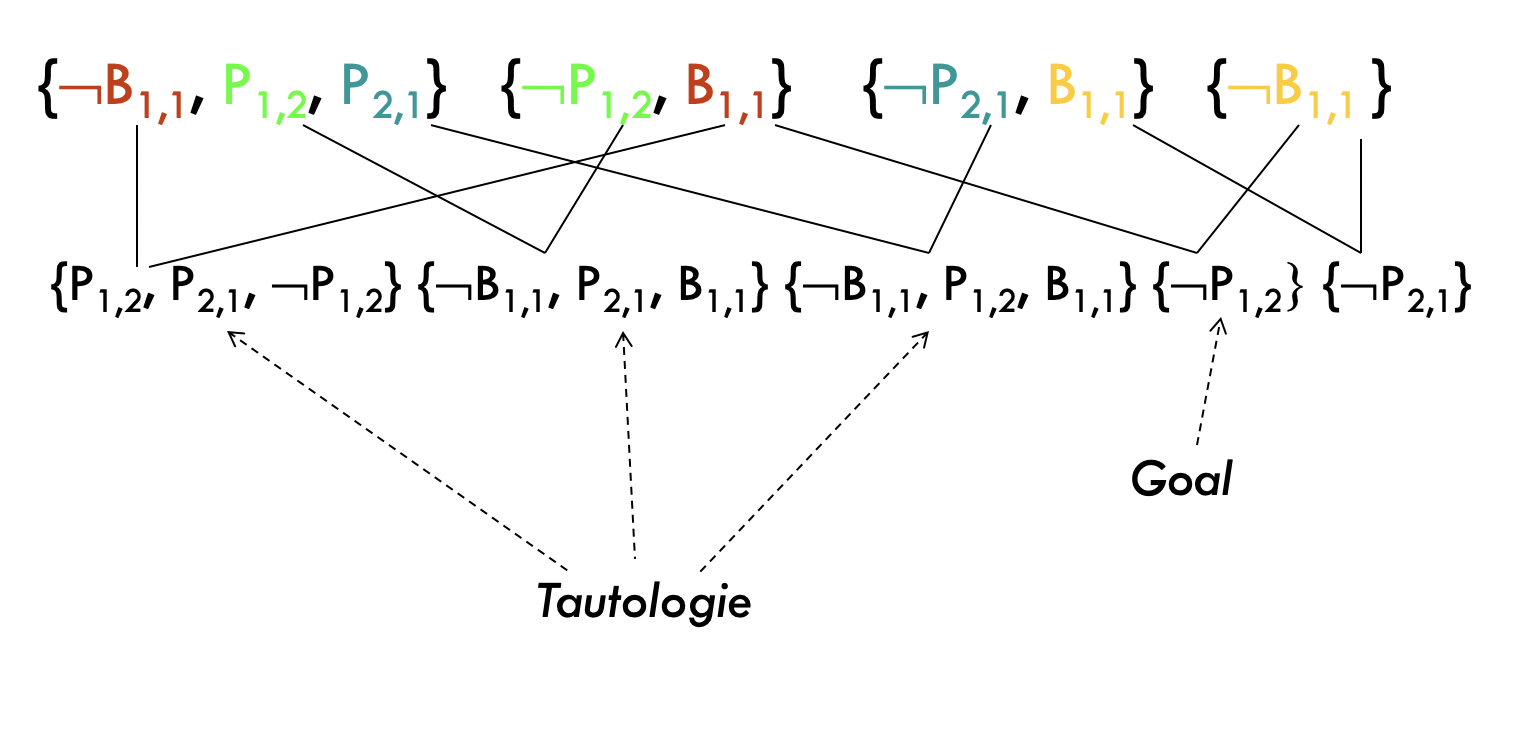
\includegraphics[scale=0.5]{Images/esgraforisoluzione.png}
\end{figure}
\subsubsection{Refutazione}
\begin{figure}[H]
\centering
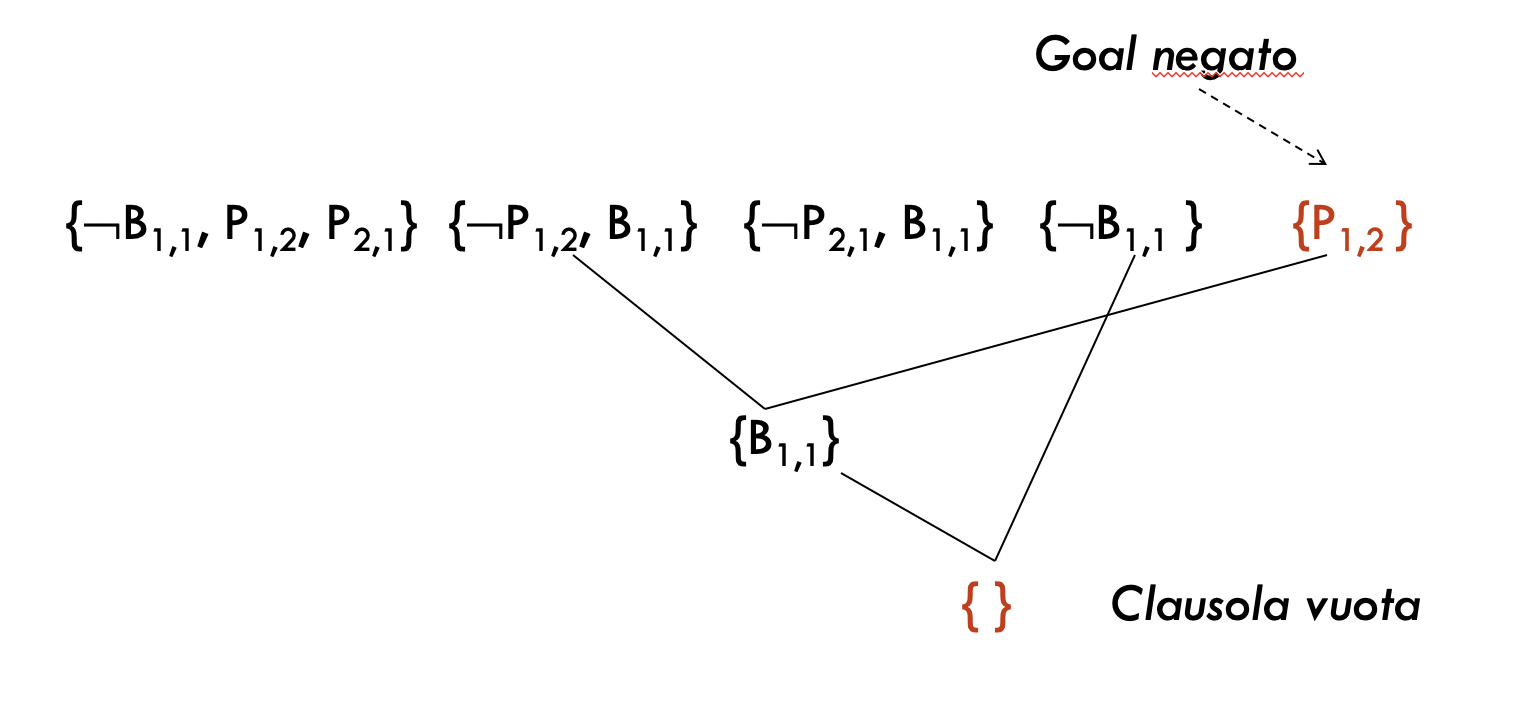
\includegraphics[scale=0.5]{Images/refutazione.png}
\end{figure}
ATTENZIONE:
\begin{figure}[H]
\centering
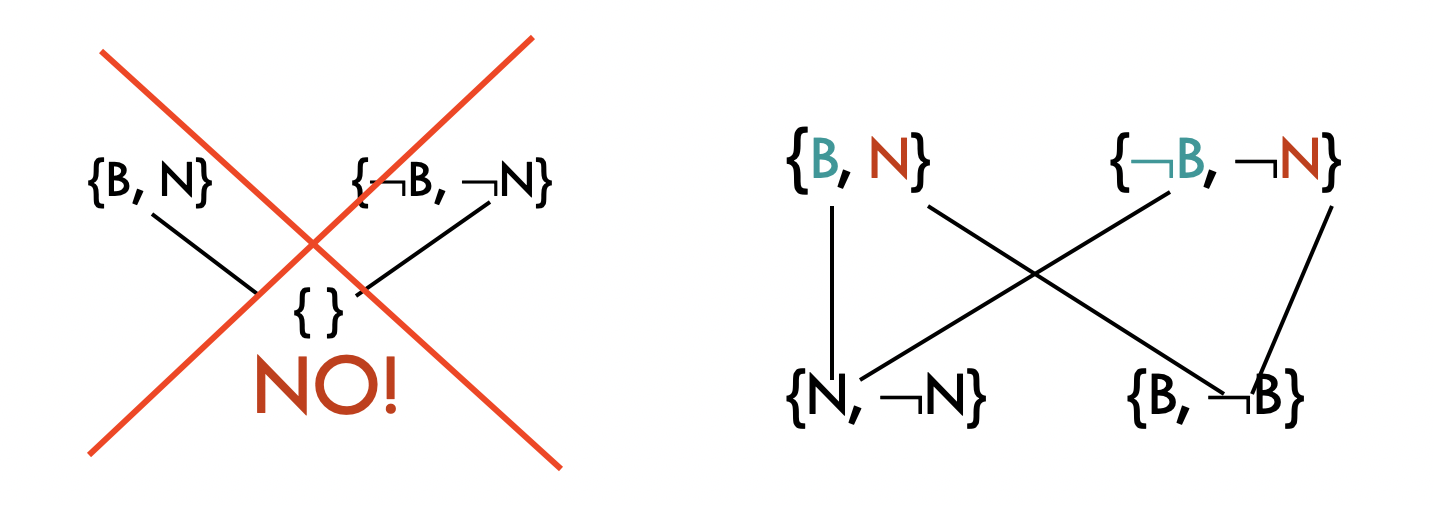
\includegraphics[scale=0.4]{Images/danger.png}
\end{figure}

\subsubsection{Osservazioni}
Abbiamo una singola regola di inferenza, ma è sufficiente? Siamo sicuri che applicando la regola in tutti i modi possibili riesco a dedurre $\alpha$ quando è conseguenza logica? Vale la completezza? Non sempre. \newline
Per fortuna il teorema di refutazione ci offre un modo alternativo di procedere: se voglio sapere se $KB \models \alpha$, aggiungo $\neg \alpha$ a KB e controllo che l’insieme ottenuto sia insoddisfacibile. La correttezza della regola ci dice anche che se da tale insieme derivo la clausola vuota allora in effetti l’insieme è insoddisfacibile. Invece il teorema di risoluzione ci garantisce che se KB è insoddisfacibile allora la clausola vuota sono sempre in grado di trovarla con applicazioni della regola di risoluzione $KB \vdash _{RES} \{\}$. \newline 
Procedere per refutazione ci garantisce la completezza (naturalmente se la procedura applica la regola in maniera sistematica).

\section{Agenti Logici: Logica del prim'ordine}
Nella logica dei predicati abbiamo assunzioni che comprendono gli oggetti, le proprietà e le relazioni. 
\begin{itemize}
    \item Gli oggetti: un libro, un evento, una persona... Possono essere identificati relativamente ad altri oggetti o con simboli, oppure mediante funzioni: "la madre di Pietro". L’insieme degli oggetti rilevanti costituiscono il dominio del discorso. (Il dominio potrebbe essere infinito).
    \item Le proprietà: "la madre di Pietro è simpatica"
    \item Le relazioni tra gli oggetti: "Pietro è amico di Paolo"
\end{itemize} 

\subsection{Il mondo dei blocchi}
\begin{itemize}
    \item Dominio: \{a, b, c, d, e\} (blocchi)
    \item Le funzioni: si individuano le funzioni rilevanti che servono per identificare oggetti. Ad esempio la funzione "Hat(x)": dato un blocco "x" identifica il blocco ad esso superiore.
    \item Le relazioni: si individuano le relazioni interessanti. 
        \begin{itemize}
            \item On = $\{<a, b>, <b, c>, <d, e>\}$ //a è su b, b è su c, d è su e
            \item Clear = \{a, d\} //non hanno nulla sopra di loro
            \item Table = \{c, e\} //sono poggiati sul tavolo
            \item Block = \{a, b, c, d, e\} //sono blocchi
    \end{itemize} 
\end{itemize}
\begin{figure}[H]
\centering
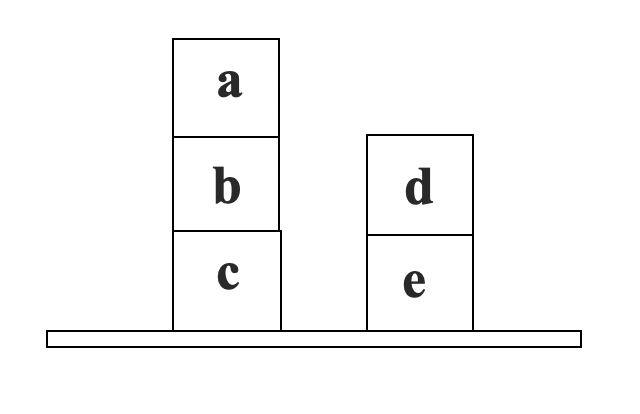
\includegraphics[scale=0.5]{Images/blocks.png}
\end{figure}

\subsection{Concettualizzazioni}
Otteniamo così la concettualizzazione del problema definita come \newline 
$<\{a, b, c, d, e\}, \{Hat\}, \{On, Clear, Table, Block\}>$ \newline
Le concettualizzazioni possibili sono infinite, un aspetto importante è il livello di astrazione giusto per gli scopi della rappresentazione. Se fosse rilevante il colore o la grandezza dei blocchi dovremmo introdurre predicati anche per questi aspetti.

\subsection{FOL}
\subsubsection{Predicati}
\begin{itemize}
    \item Connettivo $\rightarrow \land | \lor | \neg | \Rightarrow | \Leftrightarrow | \Leftarrow$
    \item Quantificatore $\rightarrow \forall | \exists $
    \item Variabile $\rightarrow x | y | ...$
    \item Costante $\rightarrow A | B | Mario | 2 ...$
    \item Funzione $\rightarrow Hat | + | - ...$
    \item Predicato $\rightarrow On | Clear | > | < | ...$
\end{itemize}
L'arità è il numero di "parametri" della funzione o del predicato.
\subsubsection{Termini}
\begin{itemize}
    \item Termine $\rightarrow Costante | Variabile | Funzione(Termine,...)$
\end{itemize}
\subsubsection{Formule}
\begin{itemize}
    \item Formula\_Atomica $ \rightarrow True | False | Termine=Termine | Predicato(Termine,...)$
    \item Formula $\rightarrow Formula\_Atomica | Formula\_Connettivo\_Formula |$ \newline $Quantificatore\_Variabile\_Formula | \neg Formula$
\end{itemize}
Di solito le variabili sono usate nell'ambito di quantificatori. In tal caso le occorrenze si dicono legate. Se non sono legate, si dicono libere. \newline
    Mela(x) $\Rightarrow$ Rossa(x) \quad x è libera in entrambe le occorrenze \newline
	$\forall$ x Mela(x) $\Rightarrow$ Rossa(x) \quad x è legata \newline
	Mela(x) $\Rightarrow \exists$x Rossa(x) \quad la prima x è libera, la seconda legata \newline
Formula chiusa: una formula che non contiene occorrenze di variabili libere, altrimenti è detta aperta.\newline
Formula ground: una formula che non contiene variabili.

\subsubsection{Interpretazione}
La semantica dichiarativa consiste nello stabilire una corrispondenza tra i termini del linguaggio e gli oggetti del mondo. \newline
Una interpretazione "I" stabilisce una corrispondenza precisa tra elementi atomici del linguaggio ed elementi della concettualizzazione. "I" interpreta:
\begin{itemize}
    \item i simboli di costante come elementi del dominio
    \item i simboli di funzione come funzioni da n-uple di D $\rightarrow$ D
    \item i simboli di predicato come insiemi di n-uple
\end{itemize}

\subsection{Sematica Composizionale}
Il significato di un termine o di una formula composta è determinato in funzione del significato dei suoi componenti.
\begin{itemize}
    \item Semantica $\forall$:  $\forall x$ A(x) è vera se per ciascun elemento del dominio A è vera. Se il dominio è finito equivale a un grosso $\land$. Tipicamente, siccome difficilmente una proprietà è universale, $\forall$ si usa quasi sempre insieme a $\Rightarrow$. (Es: $\forall x$ Persona(x) $\Rightarrow$ Mortale(x)).
    \item Semantica $\exists$: $\exists x$ A(x) è vera se esiste almeno un elemento del dominio per cui A è vera. Se il dominio è finito equivale a un grosso $\lor$. Tipicamente $\exists$ si usa con $\land$ (Es: $\exists$x Persona(x) $\land$ Speciale(x).
\end{itemize}
\begin{figure}[H]
\centering
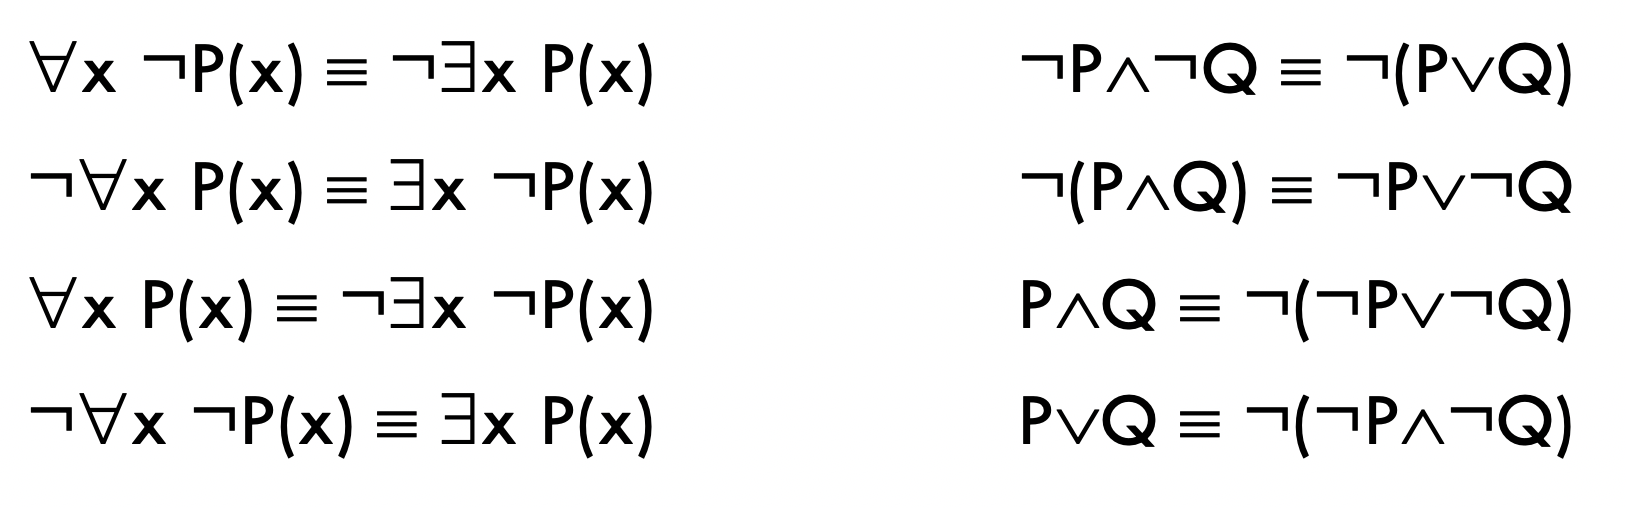
\includegraphics[scale=0.3]{Images/foarallexistsrelation.png}
\caption{Relazione tra $\forall$ ed $\exists$}
\end{figure}

\subsubsection{Semantica Standard VS Semantica Database}
\begin{itemize}
    \item Standard: ci permette di inferire.
    \item Database: simboli distinti, oggetti distinti, mondo chiuso cioè tutto ciò di cui non si sa che è vero è falso, infine esistono solo gli oggetti di cui si parla.
\end{itemize}

\subsection{Interazione con la KB tramite FOL}
\begin{itemize}
    \item Asserzioni: vengono aggiunte le informazioni alla KB, esempio TELL(KB, King(John)) oppure TELL(KB, $\forall x$ King(x) $\Rightarrow$ Person(x))
    \item Conseguenze logiche: ASK(KB, Person(John)) risponde si, se KB $\models$ Person(John). Un altro esempio è ASK(KB, $\exists$ x Person(x)) risponde con una lista di sostituzioni o legami: [\{x/John\} \{x/George\} ...]
\end{itemize}
Il metodo di risoluzione per FOL si basa sulla trasformazione in forma a clausole e poi sull'unificazione. Ci sono dei metodi particolari che vedremo alla fine: il "Backward chaining" insieme alla programmazione logica e il "Forward chaining" con basi di dati deduttive.

\subsection{Regola di inferenza per $\forall$}
Istanziazione dell’Universale (eliminazione del $\forall$) \quad
\infer{A[g]}{
    \forall x A[x]
} \newline
dove g è un termine ground (ovvero un termine che non contiene variabili) e A[g] è il risultato della sostituzione di g per x in A.\newline
Esempio: $\forall x King(x) \land Greedy(x) \Rightarrow Evil(x)$ si ottiene $ King(John) \land Greedy(John) \Rightarrow Evil(John)$

\subsection{Regola di inferenza per $\exists$}
Istanziazione dell'esistenziale (eliminazione del $\exists$) \quad 
\infer{A[k]}{
    \exists x A[x]
} \newline
dove $\exists$ non compare nell'ambito di $\forall$ e k è una costante nuova (costante di Skolem) \newline
Esempio: $\exists x Padre(x,G)$ diventa Padre(k,G). \newline
Nel caso di variabili quantificate universalmente va introdotta una funzione (di Skolem) \newline
Esempio $\forall x \exists y Padre(x, y)$ diventa $\forall x Padre(x, p(x))$

\subsection{Riduzione a inferenza proposizionale}
Per la riduzione utilizziamo un meccanismo di proposizionalizzazione. Creare tante istanze delle formule quantificate universalmente quanti sono gli oggetti menzionati ed eliminare i quantificatori esistenziali "skolemizzando". A questo punto possiamo trattare la KB come proposizionale e applicare gli algoritmi visti. Ci possono essere dei problemi? Si, le costanti sono in numero finito ma se ci sono funzioni il numero di istanze da creare è infinito: John, Padre(John), Padre(Padre(John))... In aiuto ci viene il Teorema di Herbrand.

\subsection{Teorema di Herbrand} 
Se KB $\models$ A allora c'è una dimostrazione che coinvolge solo un sotto-insieme finito della KB proposizionalizzata. Si può procedere in modo incrementale, iniziando col creare le istanze con le costanti, creare poi quelle con un solo livello di annidamento Padre(John), Madre(John) ed infine quelle con due livelli di annidamento Padre(Padre(John)), Padre(Madre(John))... Se KB $\nvDash$ A il processo non termina (Semidecidibile).

\subsection{Verso un metodo di risoluzione per il FOL}
Per trovare un metodo di risoluzione, come abbiamo fatto per il PROP, dobbiamo estendere al FOL la trasformazione in forma a clausole e dobbiamo introdurre il concetto di unificazione.

\subsubsection{Forma a clausole}
Una clausola è un insieme di letterali, che rappresenta la loro disgiunzione.
\begin{itemize}
    \item Clausola $\rightarrow$ {Letterale, ..., Letterale}
    \item Letterale $\rightarrow$ Formula\_Atomica $| \neg$ Formula\_Atomica
\end{itemize}
Una KB è un insieme di clausole.
\begin{quote}
    Teorema: per ogni formula chiusa $\alpha$ del FOL è possibile trovare in maniera effettiva un insieme di clausole $Forma\_a\_Clausole(\alpha)$ che è soddisfacibile se solo se $\alpha$ lo era (o insoddisfacibile se solo se $\alpha$ lo era).
\end{quote}
\clearpage

\subsubsection{Esempio di trasformazione (passo passo)}
Esempio di trasformazione in dettaglio per la frase “Tutti coloro che amano tutti gli animali sono amati da qualcuno” \newline 
La nostra formula di partenza è: $\forall x ( \forall y Animale(y) \Rightarrow Ama(x,y)) \Rightarrow (\exists y Ama(y, x))$
\begin{enumerate}
    \item Eliminazione delle implicazioni ($\Rightarrow, \Leftrightarrow$):
        \begin{itemize}
            \item A $\Rightarrow$ B diventa	$\neg A \lor B$
            \item A $\Leftrightarrow$ B diventa $(\neg A \lor B) \land (\neg B \lor A)$
        \end{itemize}
    $\forall x (\forall y Animale(y) \Rightarrow Ama(x,y)) \textcolor{red}{\Rightarrow} (\exists y Ama(y, x))$ \newline
    $\forall x \neg (\forall y Animale(y) \textcolor{red}{\Rightarrow} Ama(x,y)) \lor (\exists y Ama(y, x))$ \newline
    $\forall x \neg (\forall y \neg Animale(y) \lor Ama(x,y)) \lor (\exists y Ama(y, x))$
    \item Negazioni all'interno:
        \begin{itemize}
            \item $\neg \neg A$ diventa A
            \item $\neg (A \land B)$ diventa $\neg A \lor \neg B)$
            \item $\neg (A \lor B)$ diventa $\neg A \land \neg B)$
            \item $\neg \forall x A$ diventa $\exists x \neg A$
            \item $\neg \exists x A $ diventa $\forall x \neg A$
        \end{itemize}
    $\forall x \textcolor{red}{\neg} (\forall y \neg Animale(y) \lor Ama(x,y)) \lor (\exists y Ama(y, x))$ \newline
    $\forall x (\exists y \neg (\neg Animale(y) \lor Ama(x,y))) \lor (\exists y Ama(y, x))$ \newline
    $\forall x (\exists y Animale(y) \land \neg Ama(x,y)) \lor (\exists y Ama(y, x))$
    \item Standardizzazione delle variabili: ogni quantificatore una variabile diversa \newline
    $\forall x (\exists y Animale(y) \land \neg Ama(x,y)) \lor (\exists z Ama(z, x))$
    \item Skolemizzazione: eliminazione dei quantificatori esistenziali \newline
    In questo caso essendo che i due quantificatori esistenziali sono nell'ambito di uno universale dobbiamo introdurre due funzioni di Skolem. \newline
    $\forall x (Animale(F(x)) \land \neg Ama(x,F(x))) \lor (Ama(G(x), x))$
    \item Eliminazione quantificatori universali: possiamo portarli tutti davanti e poi eliminarli usando la convenzione che le variabili libere sono quantificate universalmente. \newline
    $(Animale(F(x)) \land \neg Ama(x,F(x))) \lor (Ama(G(x), x))$
    \item Forma normale congiuntiva (congiunzione di disgiunzioni di letterali): \newline
    $(Animale(F(x)) \lor (Ama(G(x), x))) \land (\neg Ama(x,F(x)) \lor (Ama(G(x), x)))$
    \item Notazione a clausole \newline
    $\{Animale(F(x)),(Ama(G(x), x))\} \{\neg Ama(x,F(x)),(Ama(G(x), x)))\}$
    \item Separazione delle variabili: clausole diverse, variabili diverse \newline
    $\{Animale(F(x_1)),(Ama(G(x_1), x_1))\} \{\neg Ama(x_2,F(x_2)),(Ama(G(x_2), x_2)))\}$
\end{enumerate}

\subsection{Sostituzione}
Possiamo eseguire la sostituzione in un insieme finito di associazioni tra variabili e termini, in cui ogni variabile compare una sola volta sulla sinistra. Ad esempio $\{x_1/A, x_2/f(x_3), x_3/B\}$, significa che $x_1$ va sostituita con A , $x_2$ va sostituito con f($x_3$) e $x_3$ con B (nota: sulla sinistra sono solo variabili!)\newline
Sia $\sigma$ una sostituzione e A un'espressione: $A \sigma$ è l'istanza generata dalla sostituzione (delle variabili con le corrispondenti espressioni). Possiamo scriverlo anche come Subst($\sigma$, A). Esempio: \newline
Subst(\{x/A, y/f(B), z/W\}, P(x, x, y, v)) = P(A, A, f(B), v) \newline
Subst(\{x/g(y), y/z, z/f(x)\}, Q(x, y, z)) = Q(g(y), z, f(x))

\subsection{Unificazione}
L'unificazione è una operazione mediante la quale si determina se due espressioni possono essere rese identiche mediante una sostituzione di termini a variabili. Il risultato è la sostituzione che rende le due espressioni identiche detta unificatore, oppure restituisce FAIL se le espressioni non sono unificabili. \newline
Ad esempio: P(A, y, z) e P(x, B, z) sono unificabili con $\tau$=\{x/A, y/B, z/C\} possiamo notare come $\tau$ sia un unificatore, ma non l'unico, un altro è $\sigma$=\{x/A, y/B\}. Possiamo infine notare come $\sigma$ è più generale di $\tau$ cioè istanzia 'meno' variabili. Noi però vorremmo l’unificatore più generale di tutti (MostGeneralUnifier - MGU) e abbiamo un teorema che dice che l’unificatore più generale è unico, a parte i nomi delle variabili (l’ordine non conta).

\subsubsection{Algoritmo di unificazione}
L’algoritmo di unificazione prende in input due espressioni p, q e restituisce un MGU $\Theta$ se esiste. Possiamo chiamare l'algoritmo come UNIFY(p, q) = $\Theta$ tale che SUBST($\Theta$, p) = SUBST($\Theta$, q), altrimenti FAIL. L’algoritmo esplora in parallelo le due espressioni e costruisce l’unificatore strada facendo. Appena trova espressioni non unificabili fallisce. Una causa di fallimento sono sostituzioni del tipo x=f(x), cioè sostituzioni in cui x occorre già all'interno dell'espressione. Questo controllo si chiama Occurr-Check e in tal caso FAIL. (È un controllo di complessità quadratica)
\subsubsection{Esempi}
Esempio 1
\begin{itemize}
    \item UNIFY(P(A, y, z), P(x, B, z), \{\})
    \item UNIFY((A, y, z), (x, B, z), UNIFY(P, P, \{\}))
    \item UNIFY((A, y, z), (x, B, z), \{ \})
    \item UNIFY((y, z), (B, z), UNIFY(A, x, \{\}))
    \item UNIFY((y, z), (B, z), UNIFY(x, A, \{\}))
    \item UNIFY((y, z), (B, z), UNIFY-VAR(x, A, \{\}))
    \item UNIFY((y, z), (B, z), \{x/A\})
    \item UNIFY((z), (z), \{y/B, x/A\})
    \item UNIFY(z, z, \{y/B, x/A\})
    \item \{y/B, x/A\}	
\end{itemize}
\clearpage
Esempio 2
\begin{itemize}
    \item UNIFY(P(f(x), x), P(z, z), \{\})
    \item UNIFY((f(x), x), (z, z),UNIFY(P, P, \{\}))
    \item UNIFY((f(x), x), (z, z), \{\})
    \item UNIFY((x), (z), UNIFY(f(x), z, \{\})
    \item UNIFY((x), (z), UNIFY(z, f(x), \{\}))
    \item UNIFY((x), (z), \{z/f(x)\})
    \item UNIFY-VAR(x, z, \{z/f(x)\})
    \item UNIFY(x, f(x), \{z/f(x)\})
    \item OCCUR-CHECK(x, f(x))
    \item FAIL
\end{itemize}

\subsection{Metodo di risoluzione per FOL}
Siamo ora in grado di definire in generale la regola di risoluzione per FOL.
\begin{figure}[H]
\centering
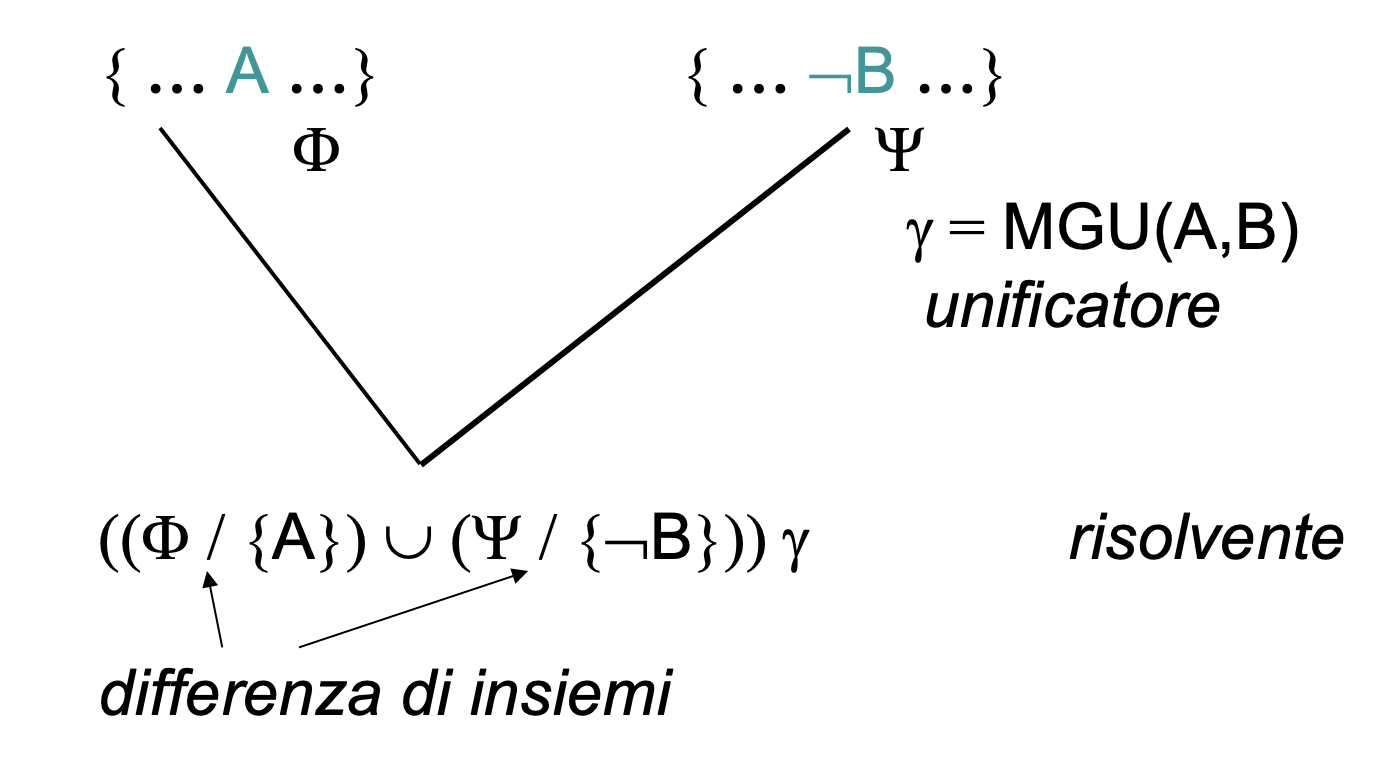
\includegraphics[scale=0.35]{Images/FOLresolmethod.png}
\end{figure}

\subsubsection{Esempio metodo di risoluzione}
\begin{figure}[H]
\centering
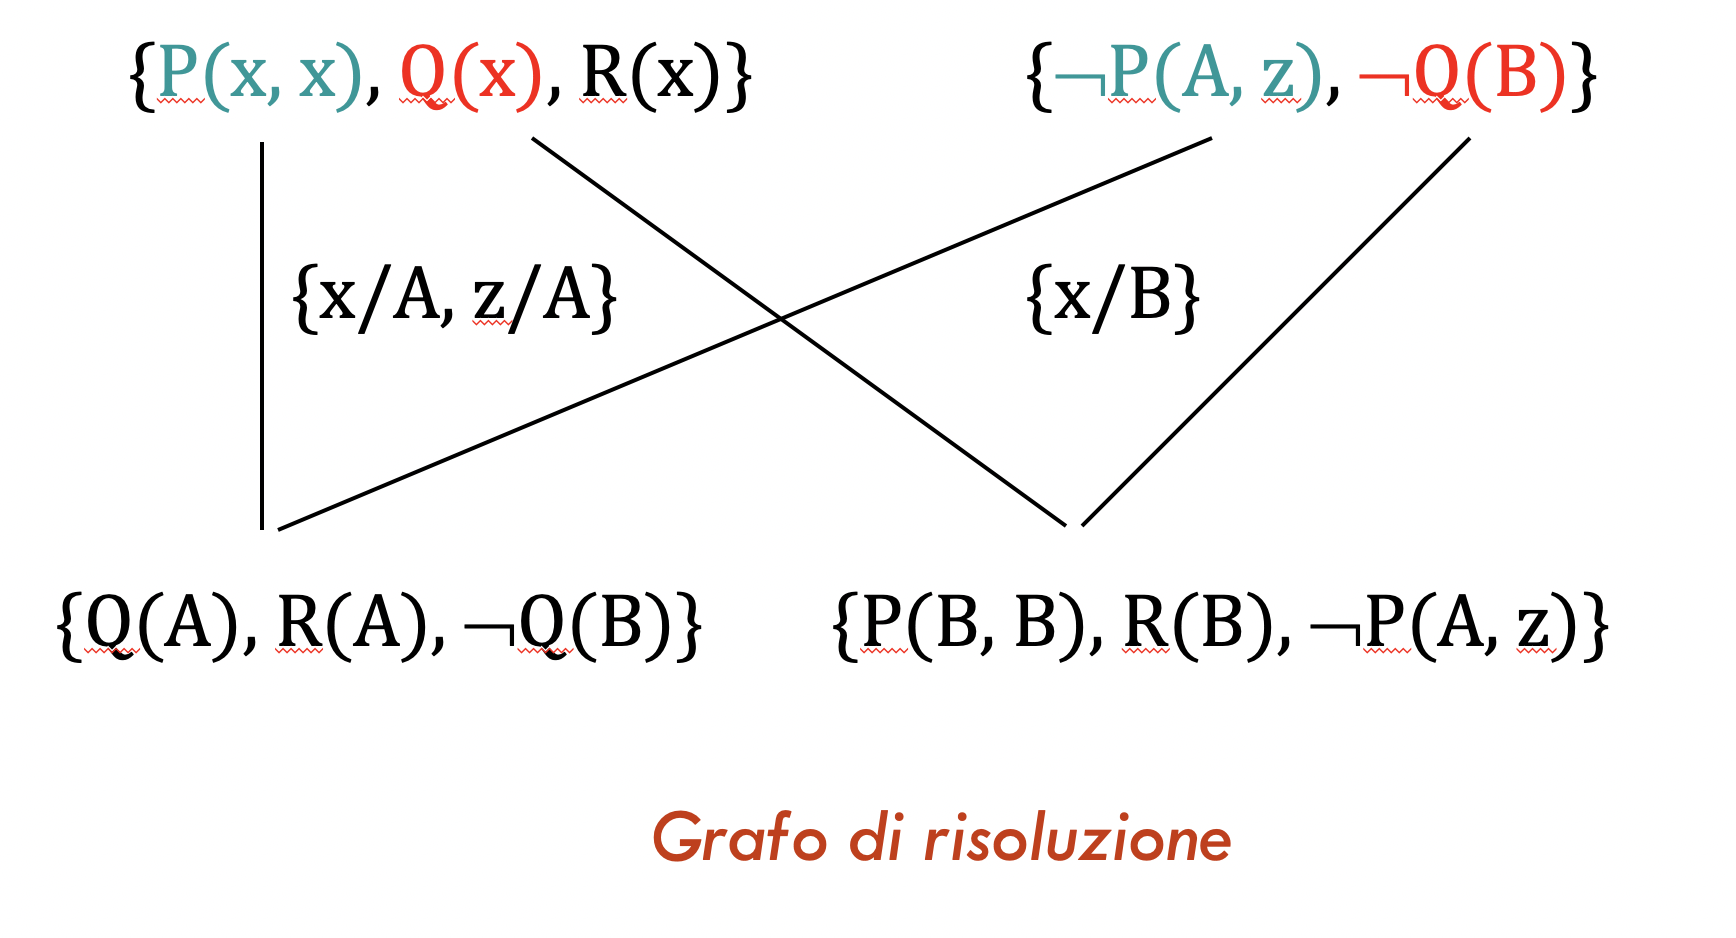
\includegraphics[scale=0.35]{Images/FOLresexample.png}
\end{figure}

\subsubsection{Problemi}
Le seguenti clausole dovrebbero produrre la clausola vuota invece...
\begin{figure}[H]
\centering
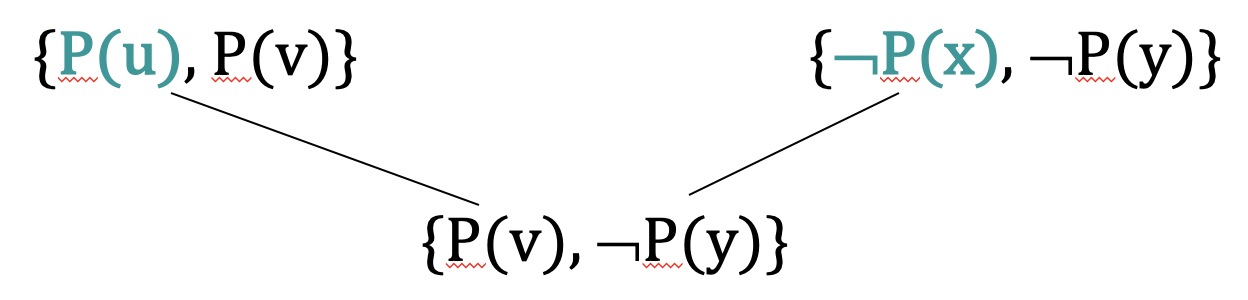
\includegraphics[scale=0.4]{Images/problem_a.png}
\end{figure}
Se un sottoinsieme dei letterali di una clausola può essere unificato allora la clausola ottenuta dopo tale unificazione si dice fattore della clausola originaria.\newline
Il metodo di risoluzione va applicato ai fattori delle clausole:
\begin{figure}[H]
\centering
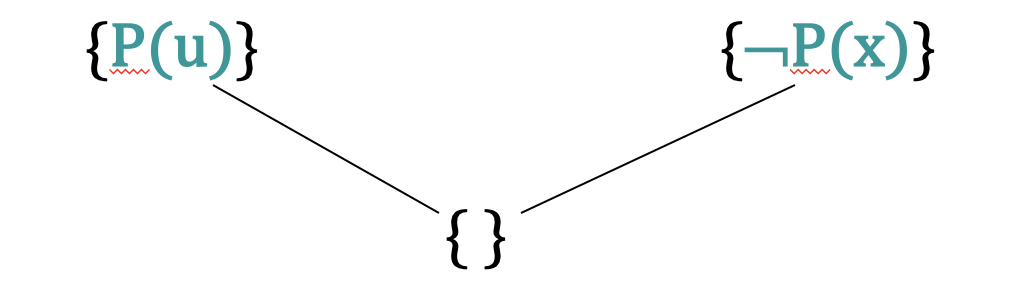
\includegraphics[scale=0.4]{Images/problem_b.png}
\end{figure}

\subsubsection{Completezza del metodo di risoluzione}
La deduzione per risoluzione è corretta	se $\Gamma \vdash _{RES}$ A allora $\Gamma \models A$ \newline
La deduzione per risoluzione non è completa perché può essere che $\Gamma \models A$ ma non $\Gamma \vdash _{RES}$ A \newline
Un esempio è \{ \} $\models$ \{P, $\neg$P\} ma non è vero che \{ \} $\vdash _{RES}$ \{P, $\neg$P\}

\subsection{Refutazione}
Come per PROP, il teorema di refutazione ci suggerisce un metodo alternativo completo. 
Il teorema di refutazione dice che $\Gamma \cup \{\neg A\}$ è insoddisfacibile sse $\Gamma \models A$. \newline
Possiamo dire quindi che $\Gamma$ è insoddisfacibile sse $\Gamma \vdash _{RES} \{\}$. Abbiamo quindi un metodo meccanizzabile, corretto e completo: basta aggiungere il negato della formula da dimostrare e provare a generare la clausola vuota.

\subsubsection{Esempio di Refutazione}
La nostra KB è formata da:
\begin{itemize}
    \item \{P(A, J)\} A è padre di J
    \item \{M(B, J)\} B è madre di J
    \item \{$\neg$P(x, y), G(x, y)\} padre implica genitore
    \item \{$\neg$M(v, w), G(v, w)\} madre implica genitore
\end{itemize} \clearpage
Il nostro goal è sapere se A è genitore di J, in forma a clausole se \{(A, J)\} appartiene alla KB. Per refutazione possiamo quindi aggiungere alla KB la negazione del goal \{$\neg$G(A, J)\} e proviamo a dedurre la clausola vuota.
\begin{figure}[H]
\centering
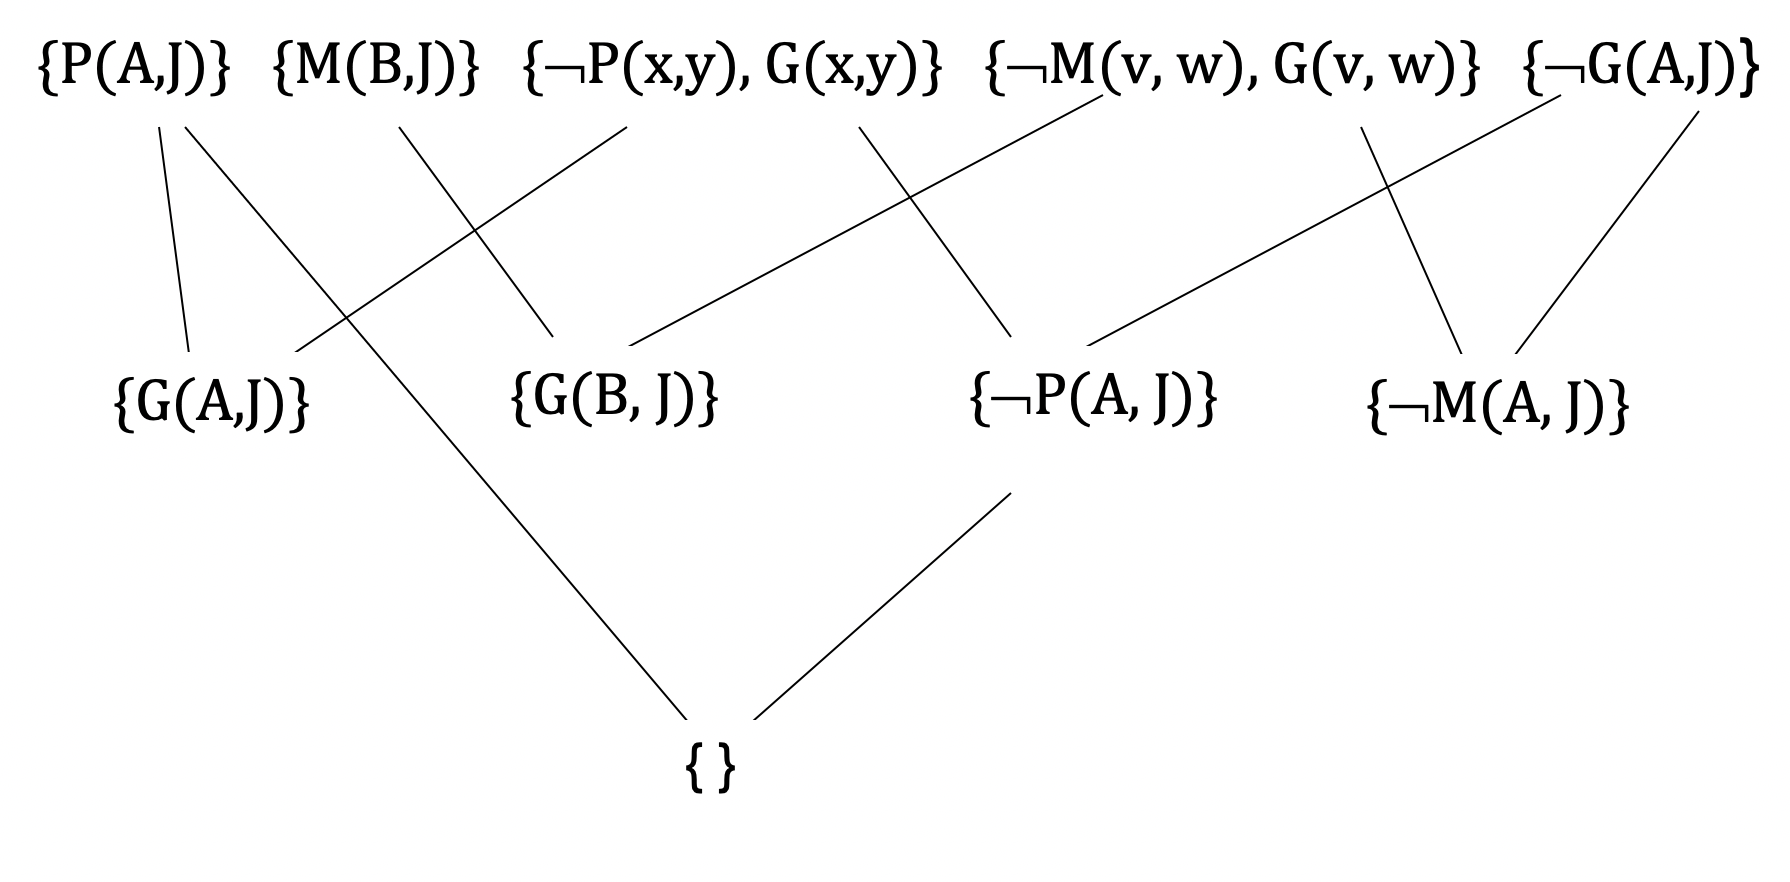
\includegraphics[scale=0.4]{Images/refutazioneesempio.png}
\end{figure}
E per domande del tipo "trova...?" come ad esempio "chi sono i genitori di J? \newline
Si cerca di dimostrare che $\exists z G(z,J) \rightarrow \{\neg G(z,J)\}$ e la risposta sono tutti i possibili legami per z che consentono di ottenere la clausola vuota.
\begin{figure}[H]
\centering
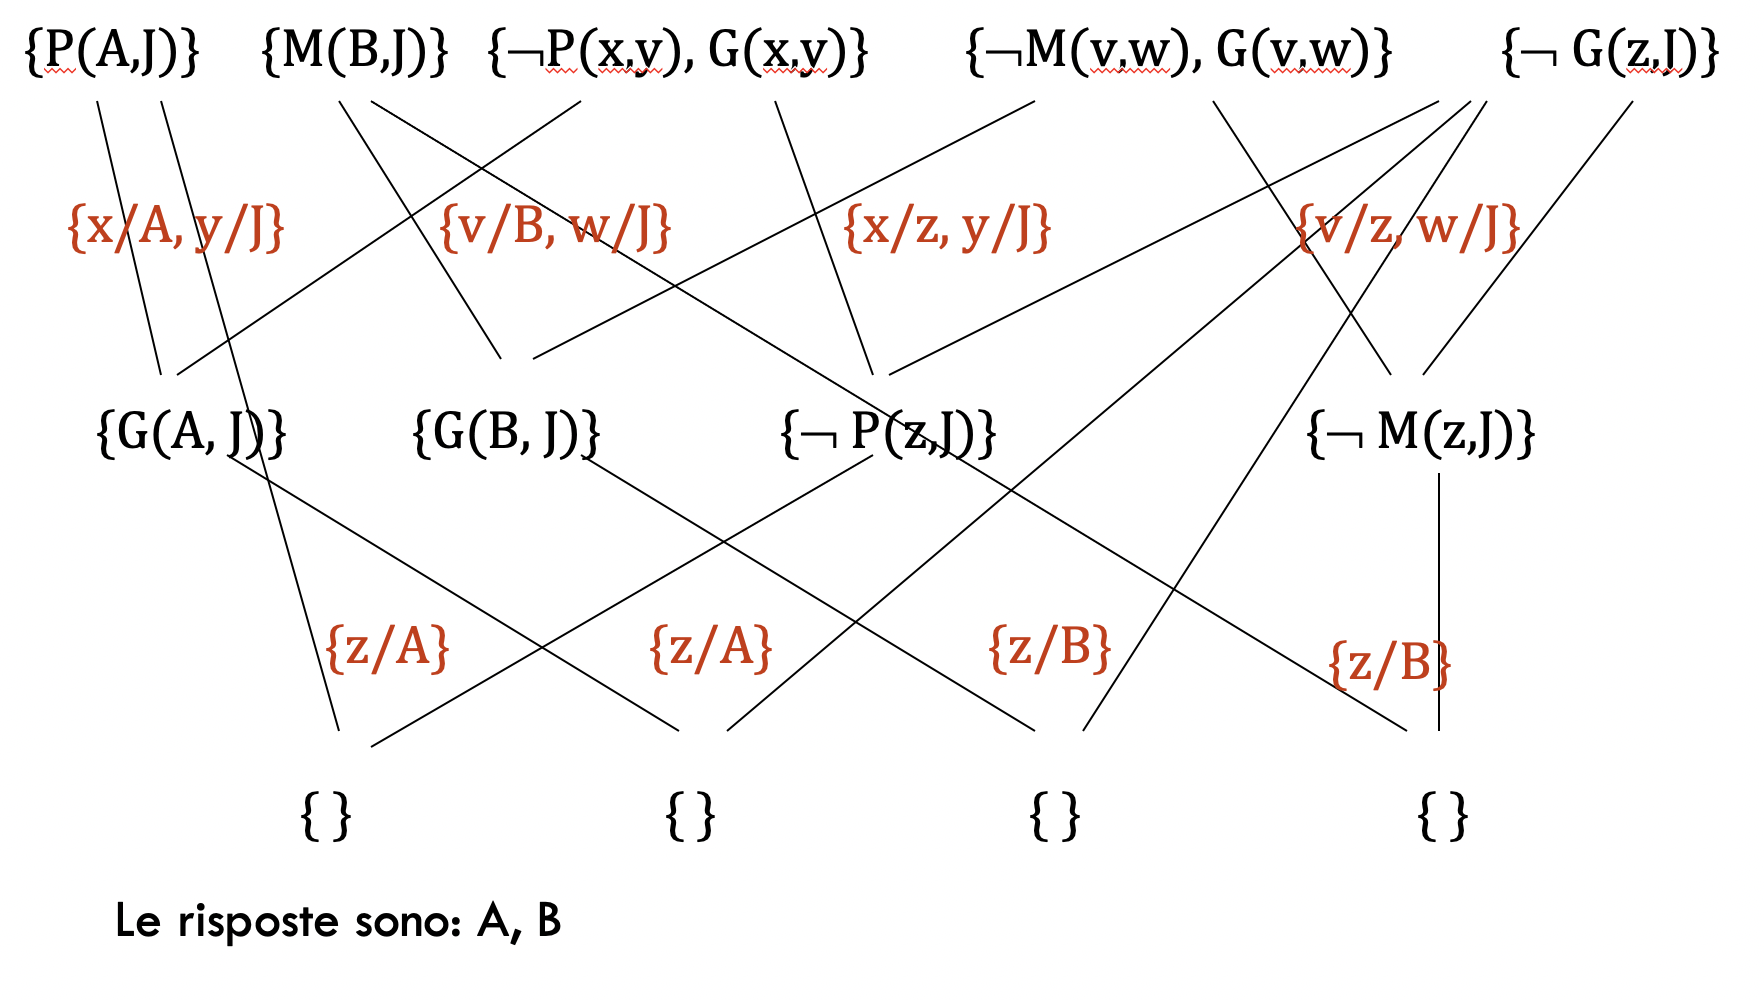
\includegraphics[scale=0.4]{Images/refutazioneesempio2.png}
\end{figure}

\subsection{Risoluzione efficiente per FOL}
Come si può rendere più efficiente il metodo di risoluzione per FOL? Sfrutteremo tecniche per esplorare in maniera efficiente il grafo di risoluzione, possibilmente senza perdere completezza. Distingueremo tra:
\begin{itemize}
    \item Strategie di cancellazione: ci sono clausole che posso eliminare?
    \item Strategie di restrizione: posso usare ad ogni passo solo alcune clausole?
    \item Strategie di ordinamento: posso 'risolvere' i letterali in un ordine specifico?
\end{itemize}
\subsubsection{Strategie di cancellazione}
Si tratta di rimuovere dalla KB (ai fini della dimostrazione) certe clausole che non potranno mai essere utili nel processo di risoluzione.
\begin{itemize}
    \item Clausole con letterali puri: sono quelle clausole che non hanno il loro negato nella KB, ad esempio in \{$\neg P, \neg Q, R\}  \{\neg P, S\}  \{\neg Q, S\} \{P\} \{Q\} \{\neg R\}$  la seconda e terza clausola contengono il letterale puro S. Le clausole con letterali puri non potranno mai essere risolte con altre clausole per ottenere \{ \}, tanto vale eliminarle che non si perdono soluzioni.
    \item Tautologie: la tautologie vengono rappresentate da quelle clausole che contengono due letterali identici e complementari. Ad esempio: $\{P(A), \neg P(A), ...\}$ oppure $\{P(x), Q(y), \neg Q(y)\}$. La loro rimozione non influenza la soddisfacibilità. \newline 
    NOTA: Le tautologie possono essere generate, quindi è un controllo da fare ad ogni passo.
    \item Clausole sussunte\footnote{sussume significa “è più generale di” o “implica”}: dovremo eliminare le clausole implicate. In generale: $\alpha$ sussume $\beta$ sse $\exists \sigma . \alpha \sigma \subseteq \beta$ cioè se un’istanza di $\alpha$ con la sostituzione $\sigma$ è un sottoinsieme di $\beta$. \newline
    Ad esempio: \{P(x), Q(y)\} sussume \{P(A), Q(v), R(w)\} infatti \newline \{P(x), Q(y)\}\{x/A, y/v\}=\{P(A), Q(v)\} $\subseteq$ \{P(A), Q(v), R(w)\}. Concludendo, $\beta$ può essere ricavata da $\alpha$, quindi $\beta$ può essere eliminata senza perdere soluzioni. \newline 
    NOTA: Le clausole sussunte possono essere generate, quindi è un altro controllo da fare ad ogni passo.
\end{itemize}

\subsubsection{Strategie di restrizione}
Ad ogni passo si sceglie tra un sottoinsieme delle possibili clausole e si applica l'algoritmo su di esse. Tra le strategie di restrizione possibili:
\begin{itemize}
    \item Risoluzione unitaria: almeno una delle due clausole è unitaria (contiene un solo letterale)
        \begin{figure}[H]
        \centering
        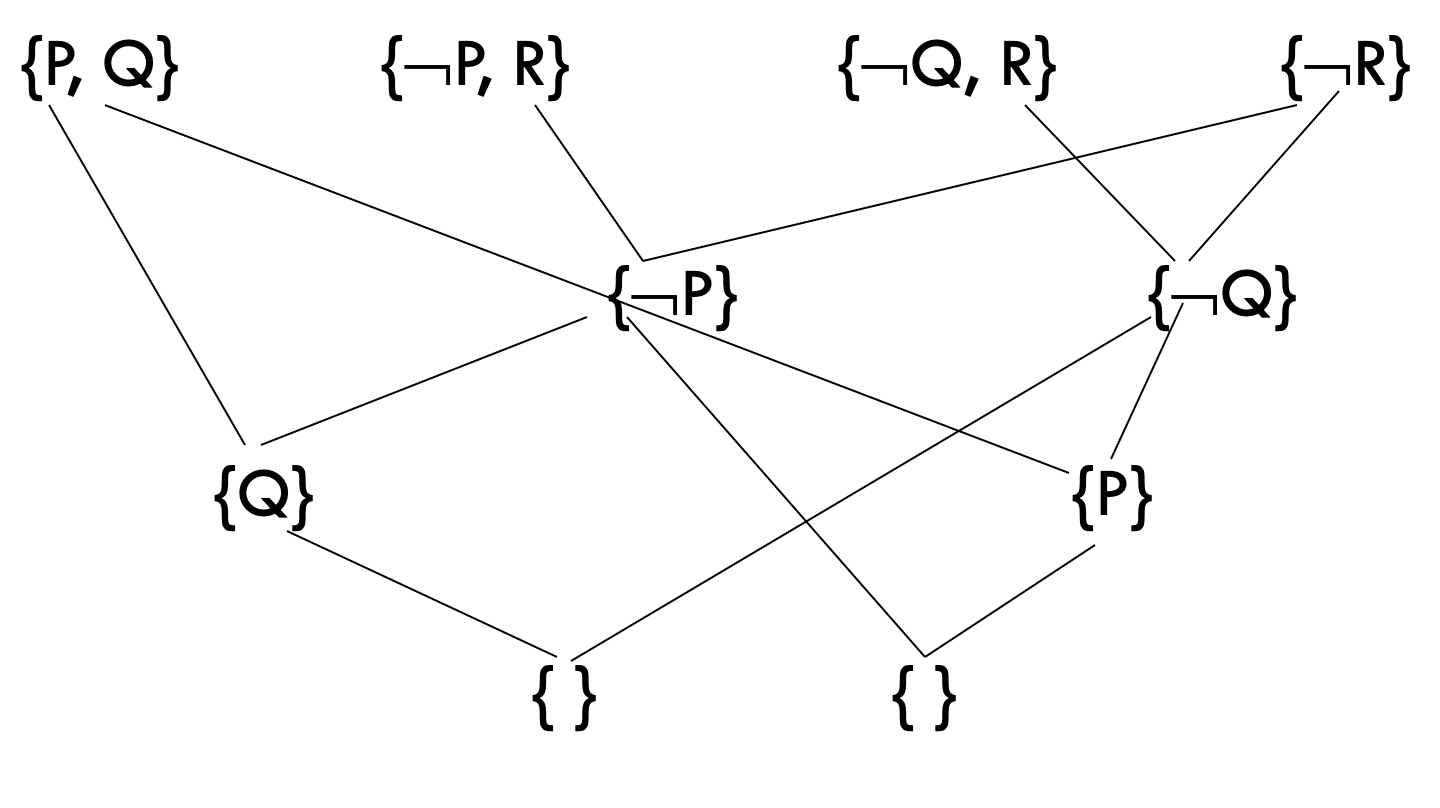
\includegraphics[scale=0.4]{Images/risoluzioneunitaria.png}
        \end{figure}
        Facile da implementare, converge rapidamente ma la strategia non è completa. \newline 
        Esempio: \{P, Q\} \{$\neg$P, Q\} \{P, $\neg$Q\} \{ $\neg$P, $\neg$Q\} $\vdash _{RES}$ \{ \} ma non con la risoluzione a clausole unitarie. \newline
        La strategia però è completa per clausole Horn cioè quelle clausole con al massimo un letterale positivo (ma possono avere più letterali nella stessa clausola), nell'esempio di prima \{P, Q\} non è una clausola Horn!
    \item Risoluzione lineare: sfruttiamo l'ultima clausola generata con una clausola da input (dalla KB iniziale) oppure una clausola antenata. La risoluzione è completa se applicata insieme ad una refutazione.
        \begin{figure}[H]
        \centering
        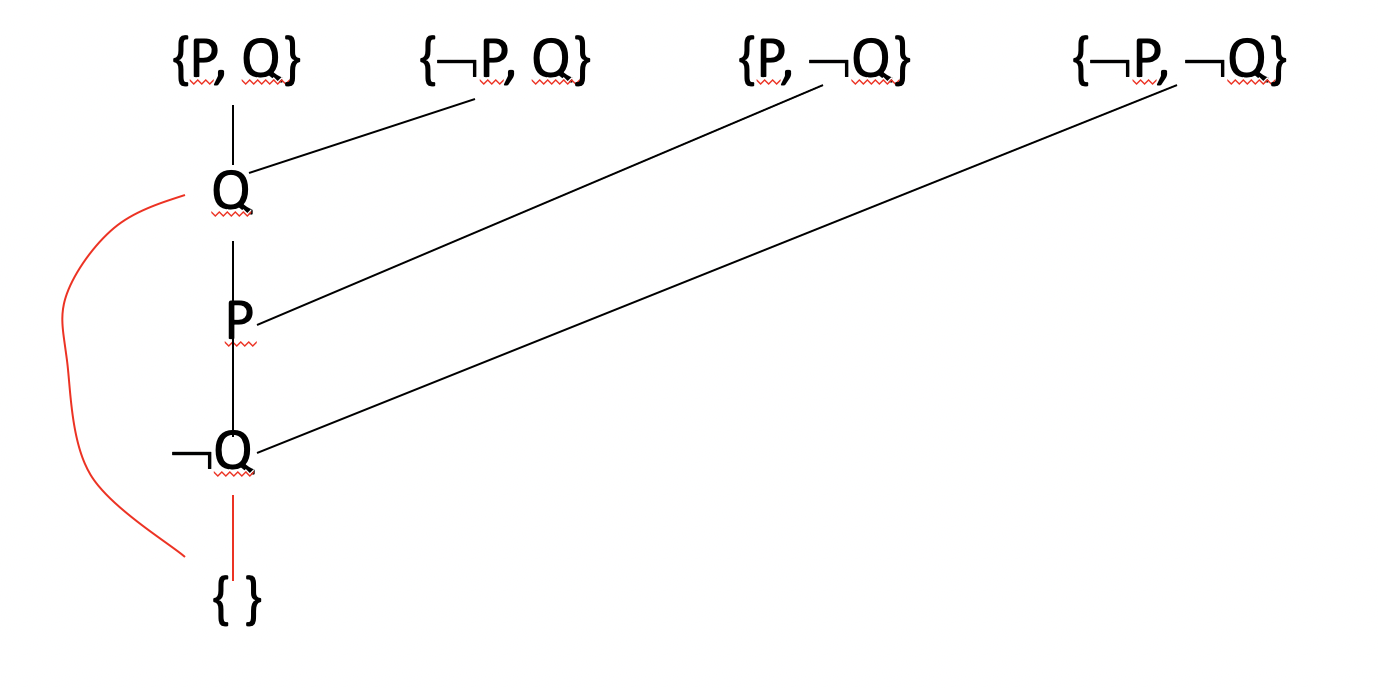
\includegraphics[scale=0.4]{Images/risoluzionelineare.png}
        \end{figure}
    \item Risoluzione guidata dal goal: sfruttiamo un insieme di supporto, cioè un sotto-insieme della KB responsabile dell'insoddisfacibilità. Tipicamente, assumendo la KB iniziale consistente, si sceglie come insieme di supporto iniziale il negato della clausola goal (è come procedere all'indietro dal goal). Come si può notare, la strategia è completa per la refutazione.
        \begin{figure}[H]
        \centering
        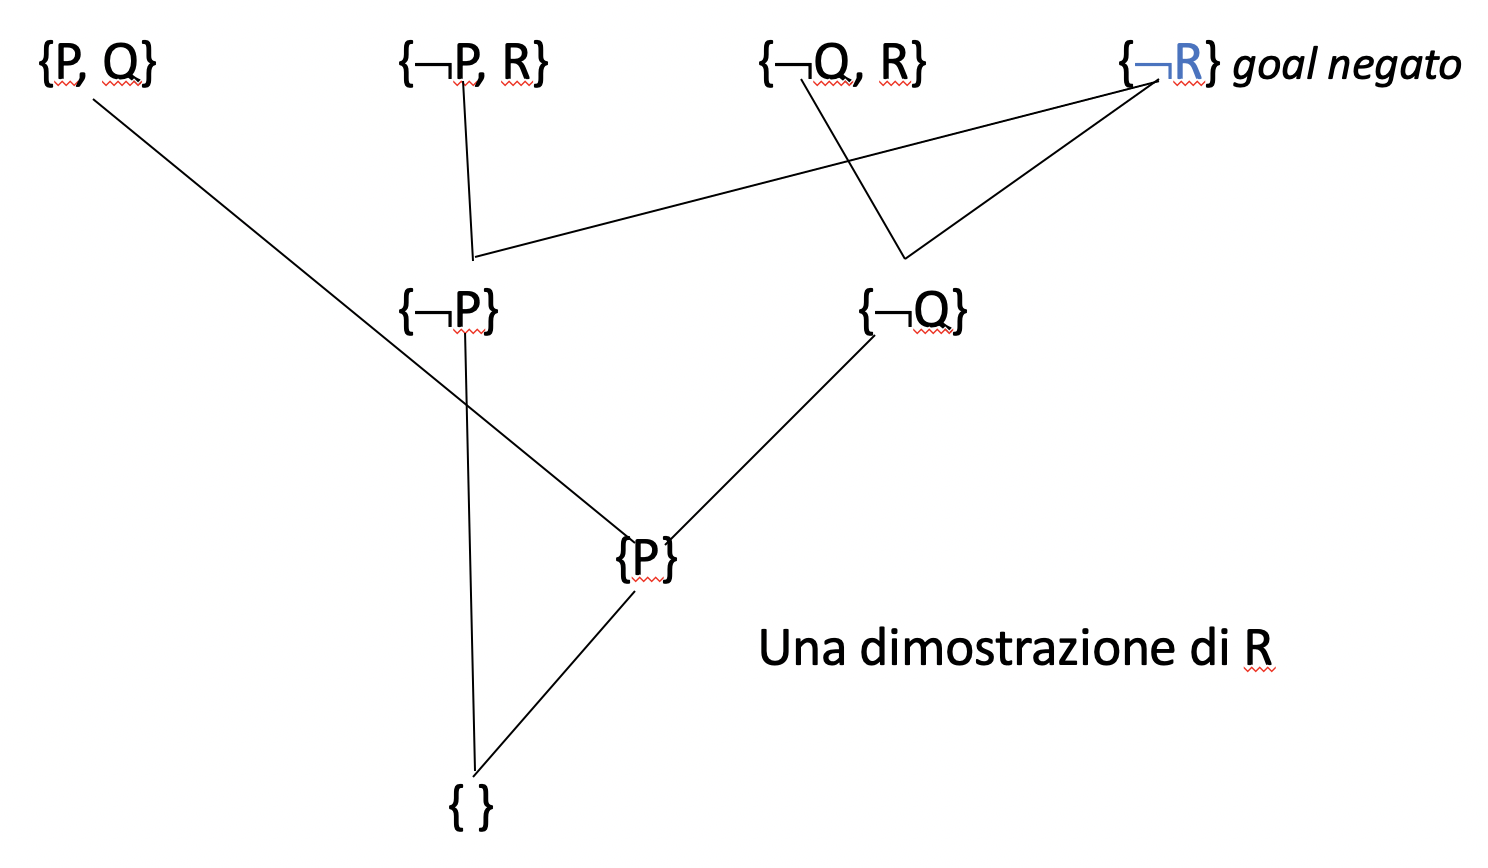
\includegraphics[scale=0.4]{Images/risoluzioneindietro.png}
        \end{figure}
\end{itemize}

\subsubsection{Strategie di ordinamento}
Ogni clausola è un insieme ordinato di letterali e si possono unificare solo i primi letterali delle clausole, l’ordinamento deve essere rispettato nel risolvente. La risoluzione ordinata è completa per clausole Horn.
\begin{figure}[H]
\centering
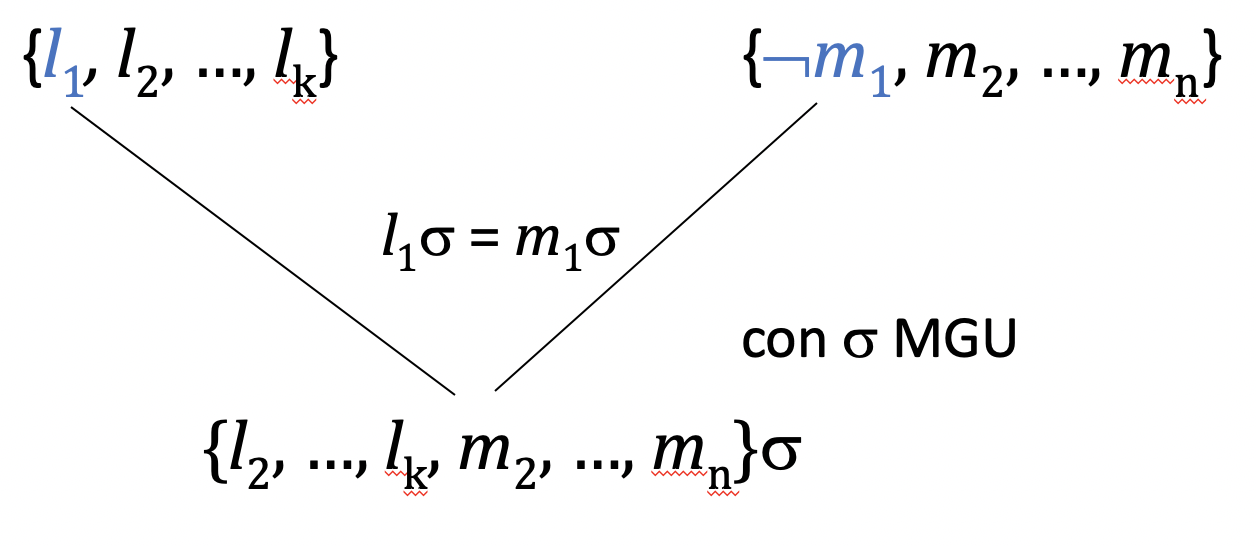
\includegraphics[scale=0.4]{Images/risoluzioneordinata.png}
\end{figure}
\begin{figure}[H]
\centering
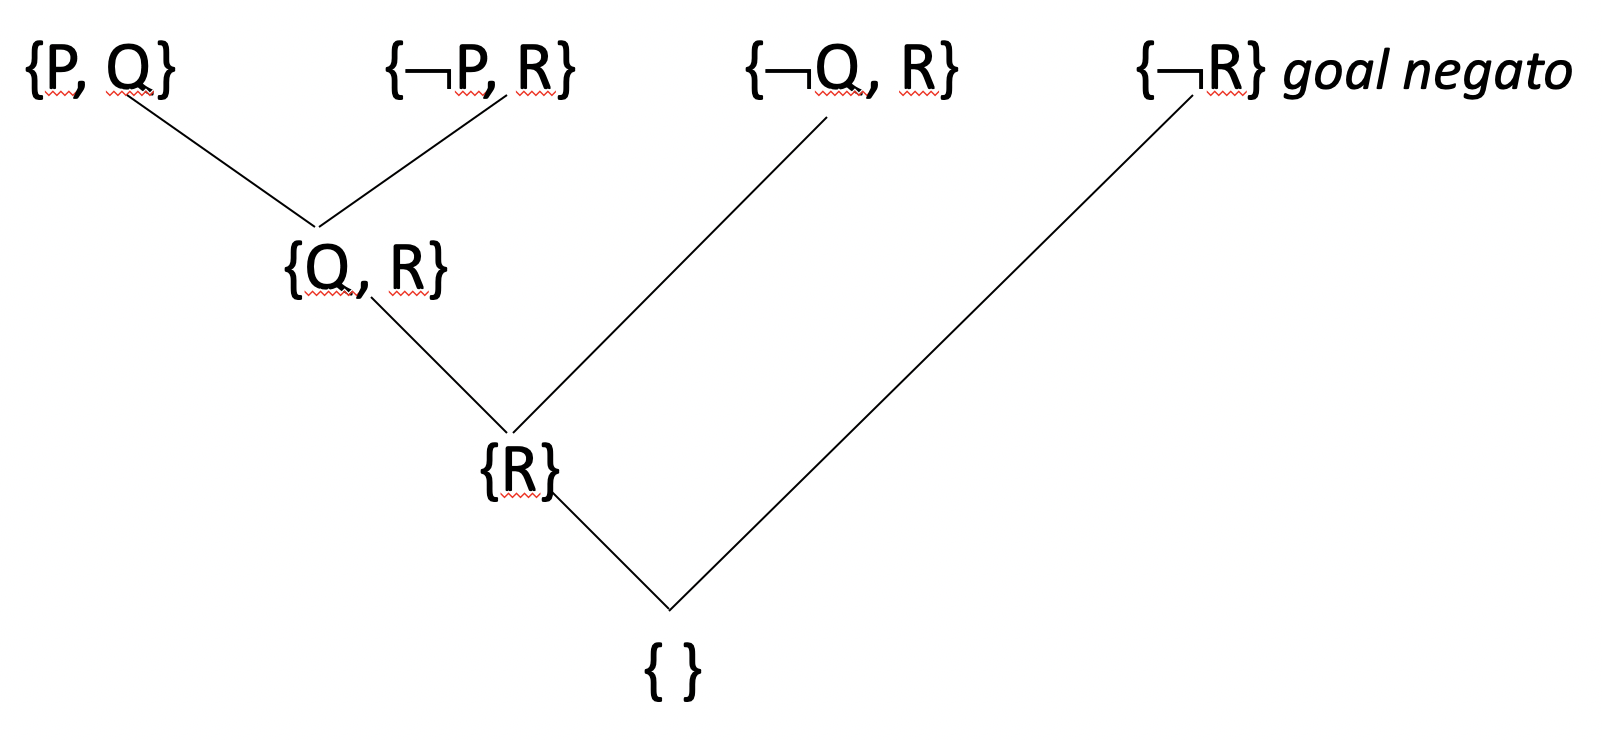
\includegraphics[scale=0.4]{Images/risoluzioneordinataesempio.png}
\caption{risoluzione ordinata esempio}
\end{figure}

\subsection{Sistemi a regole}
Le clausole Horn definite sono quelle clausole con esattamente un letterale positivo\footnote{Clausole Horn: possono avere più letterali ma al massimo uno solo positivo \newline Clausole Horn Definite: possono avere più letterali ma hanno esattamente un letterale positivo}. Possono essere riscritte come fatti e regole, cioè \newline
$\neg P_1 \lor ... \lor \neg P_k \lor Q$ \quad viene riscritta come \newline
$\neg (P_1 \land ... \land P_k) \lor Q$\quad quindi \newline
$(P_1 \land ... \land P_k) \Rightarrow Q$ con Q chiamato fatto. \newline
Se la KB contiene solo clausole Horn definite, i meccanismi inferenziali sono molto più semplici senza rinunciare alla completezza. Ovviamente è un sistema restrittivo, non può coincidere con FOL.

\subsubsection{Regole in avanti e indietro}
\begin{itemize}
    \item Concatenazione all'indietro (Backward Chaining): approccio guidato dall'obiettivo. Le regole sono applicate alla rovescia. (Programmazione Logica - PROLOG)
    \item Concatenazione in avanti (Forward Chaining): approccio guidato dai dati. Le regole sono applicate nel senso “antecedente-conseguente” (Basi di dati deduttive)
\end{itemize}

\subsection{Programmazione logica (Backward Chaining)}
I programmi logici sono KB costituiti da clausole Horn definite, vengono espressi come fatti e regole, con una sintassi alternativa:
\begin{quote}
    A \quad fatto \newline
 	A :- $B_1, B_2, ... , B_n$ \quad regola, con testa A, il resto è il conseguente
\end{quote}
Come convenzione, in programmazione logica, le variabili sono indicate con lettere maiuscole mentre le costanti con lettere minuscole.
Esempio: \newline
Se $B_1 \land B_2 \land ... \land B_n$ \quad è il goal, \newline
$\neg (B_1 \land B_2 \land ... \land B_n) \lor False$ \quad è il goal negato, ovvero \newline
$(B_1 \land B_2 \land ... \land B_n) \Rightarrow False$ \quad che viene scritto \newline
:-$B_1, B_2, ..., B_n$ \quad omettendo il conseguente. \clearpage

Nei programmi logici abbiamo due tipi di interpretazione per le regole:
\begin{enumerate}
    \item Interpretazione dichiarativa:	A :- $B_1, B_2, ..., B_n$ quindi A è vero se sono veri $B_1, B_2, ..., B_n$ in accordo al significato logico dell'implicazione.
    \item Interpretazione procedurale: la testa può essere vista come una chiamata di procedura e il corpo come una serie di procedure da eseguire in sequenza.
\end{enumerate}

\subsubsection{Risoluzione SLD}
La risoluzione SLD (Selection Linear Definite-clauses) è una strategia ordinata, basata su un insieme di supporto formato dalla clausola goal ed è lineare in input. La risoluzione SLD è completa per clausole Horn.

\subsubsection{Alberi di risoluzione SLD}
Dato un programma logico P, l’albero SLD per un goal G è definito come segue:
\begin{itemize}
    \item ogni nodo dell'albero corrisponde a un goal
    \item la radice è :- $G_1, G_2, ..., G_k$ che è il nostro goal
    \item sia :- $G_1, G_2, ..., G_k$ un nodo dell'albero; il nodo ha tanti discendenti quanti sono i fatti e le regole in P la cui testa è unificabile con $G_1$. \newline 
    Se A :- $B_1, ..., B_k$ e A è unificabile con $G_1$ e $\gamma$ = MGU(A, $G_1$) un discendente è il goal :-($B_1, ..., B_k, G_2, ..., G_k) \gamma$
    \item i nodi che sono clausole vuote sono successi
    \item i nodi che non hanno successori sono fallimenti
\end{itemize}

\subsubsection{Esempio di albero SLD}
\begin{enumerate}
    \item Genitore(X, Y) :- Padre(X, Y).
    \item Genitore(X, Y) :- Madre(X, Y).
    \item Antenato(X, Y) :- Genitore(X, Y).
    \item Antenato(X, Y) :- Genitore(X, Z), Antenato(Z, Y).
    \item Padre(gio, mark).
    \item Padre(gio, luc).
    \item Madre(lia, gio).
    \item :- Antenato(lia, mark). \quad (goal negato)
\end{enumerate}
\begin{figure}[H]
\centering
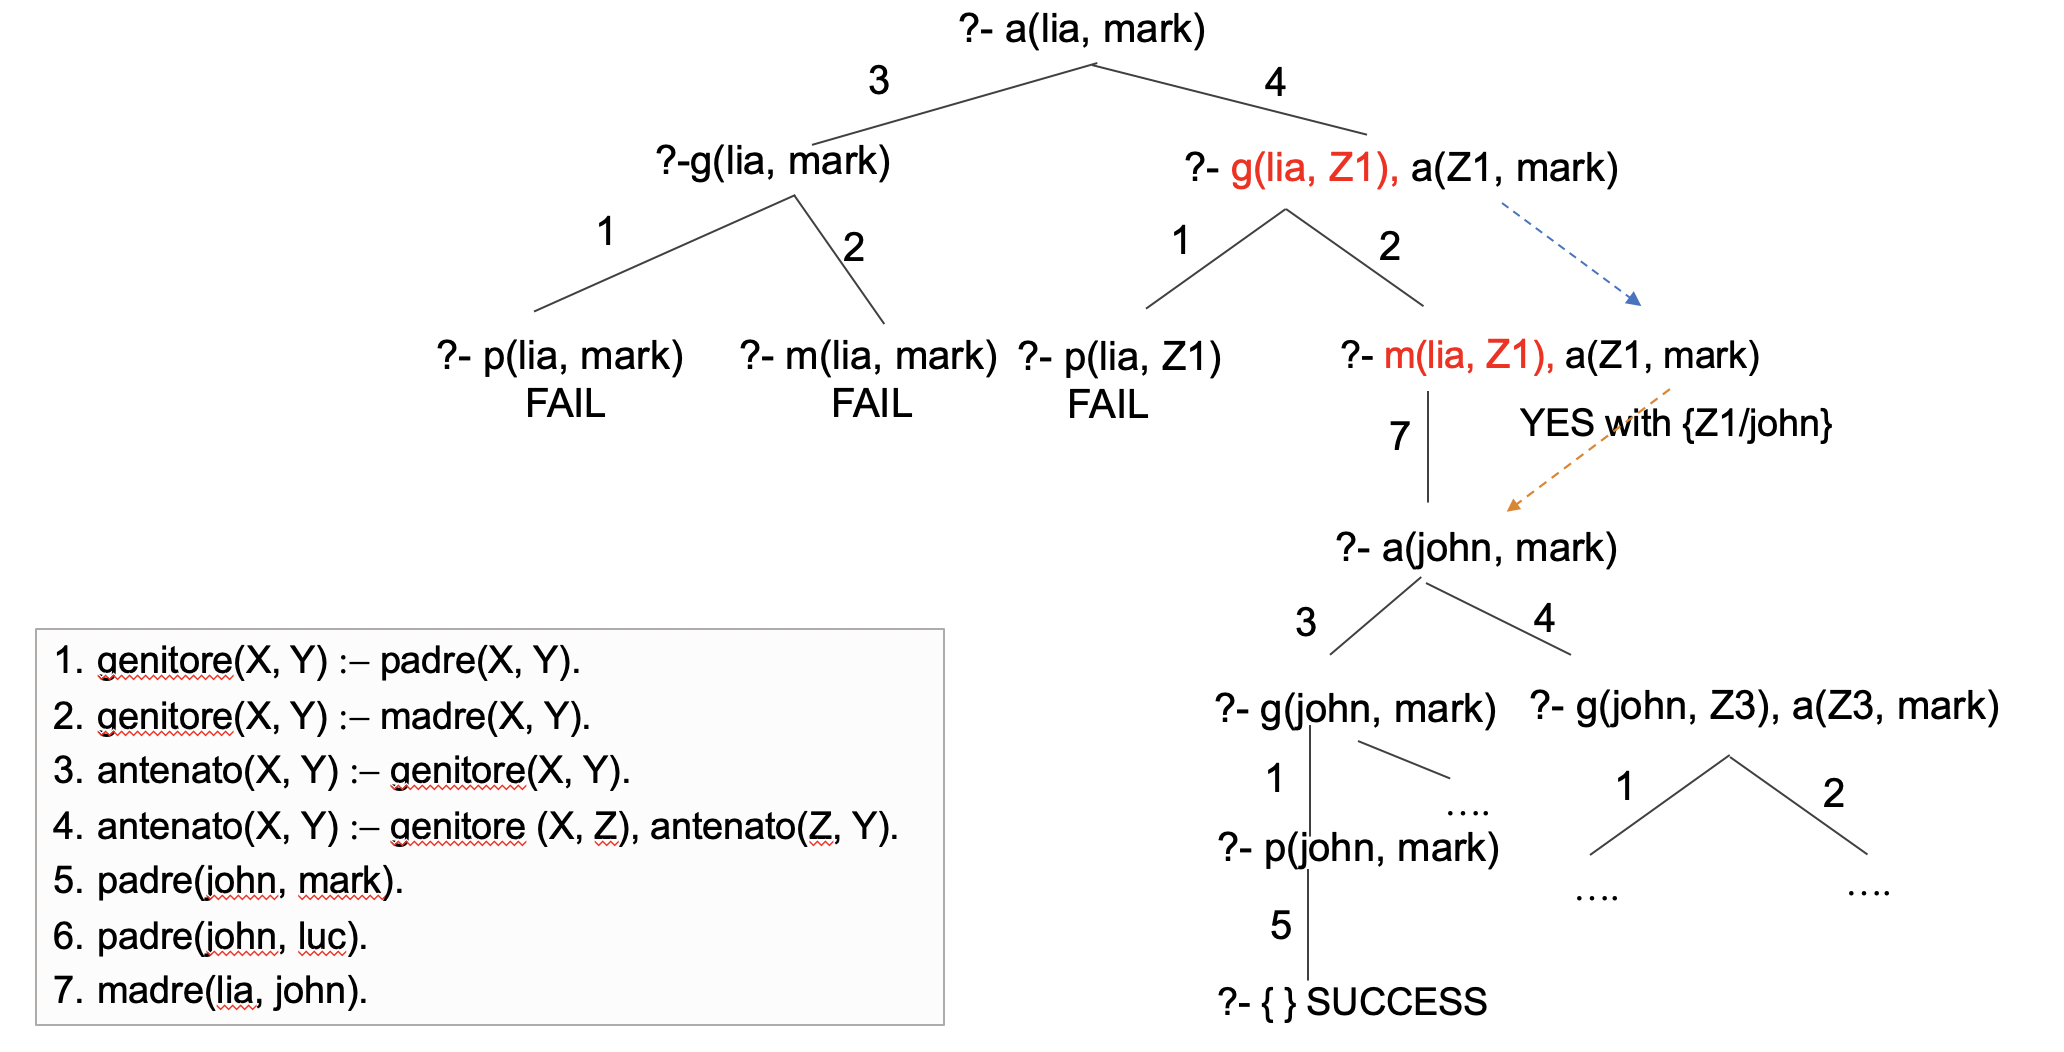
\includegraphics[scale=0.4]{Images/SLDtreeesempio.png}
\caption{Albero SLD per il goal antenato(lia,mark)}
\end{figure}
La strategia è completa per clausole Horn definite. Se $P \cup \{\neg G\}$ è insoddisfacibile, allora una delle foglie deve essere la clausola vuota (successo). La sostituzione corrispondente è la risposta calcolata. \newline
A seconda di come l’albero viene visitato si potrebbe anche non trovare la clausola vuota: la strategia di ricerca può essere responsabile dell'incompletezza! In PROLOG, il più famoso linguaggio di programmazione logica, la visita dell'albero di risoluzione avviene con una ricerca in profondità, con backtracking in caso di fallimento. Quindi la strategia di PROLOG non è completa, le regole vengono applicate nell'ordine in cui sono immesse, infine PROLOG omette l’Occur-Check per motivi di efficienza.

\subsection{Sistemi a regole in avanti (Forward Chaining - FOL\_FC\_Ask)}
Modus Ponens generalizzato: \quad
\infer{ (q) \Theta}{
    p'_{1}, p'_{2}, ..., p'_{n}
    & \deduce{(p_1 \land p_2 \land ... \land p_n \Rightarrow q)}
}
con $\Theta$ = MGU($p'_{i}, p_{i}$), per ogni i \newline
In realtà per applicare la regola dovremo: istanziare gli universali, istanziare le regole e poi applicare il Modus Ponens classico. \newline
Supponiamo di avere nella KB: King(John), Greedy(y) e King(x) $\land$ Greedy(x) $\Rightarrow$ Evil(x). \newline 
Con  $\Theta$=\{x/John, y/John\} si ottiene: \newline 
$King(John), Greedy(John)$ e $King(John) \land Greedy(John) \Rightarrow Evil(John)$. \newline 
Quindi la conclusione della regola è Evil(John).

\subsubsection{Esempio di concatenazione in avanti}
\begin{quote}
    È un crimine per un Americano vendere armi a una nazione ostile. Il paese Nono, un nemico dell’America, ha dei missili, e tutti i missili gli sono stati venduti dal colonnello West, un Americano.
\end{quote}
Dimostrare che West è un criminale.
Formalizzazione:
\begin{itemize}
    \item $Americano(x) \land Arma(y) \land Vende(x, y, z) \land Ostile(z) \Rightarrow Criminale(x)$
    \item $\exists x Possiede(Nono,x) \land Missile(x)$ lo istanziamo con $Possiede(Nono, M_1) \land Missile(M_1)$
    \item $Missile(x) \land Possiede(Nono,x) \Rightarrow Vende(West, x, Nono)$
    \item $Missile(x) \Rightarrow Arma(x)$
    \item $Nemico(x, America) \Rightarrow Ostile(x)$
    \item $Americano(West)$
    \item $Nemico(Nono, America)$
\end{itemize}
Un semplice processo inferenziale chiamato FOL\_FC\_Ask, applica ripetutamente il Modus Ponens generalizzato per ottenere nuovi fatti fino a che si dimostra quello che si desidera o nessun fatto nuovo può essere aggiunto. E' una strategia di ricerca sistematica in ampiezza, in questo esempio non ci sono funzioni e il processo converge: siamo nelle condizioni di un database DATALOG (cioè basi di dati deduttive).
Come si procede:
\begin{enumerate}
    \item $Possiede(Nono, M_1) \land Missile(M_1)$
    \item $Missile(x) \land Possiede(Nono,x) \Rightarrow Vende(West,x,Nono)$ è soddisfatta con $\{x/M-1\}$ e viene aggiunto $Vende(West, M_1, Nono)$
    \item $Missile(x) \Rightarrow Arma(x)$ è soddisfatta con $\{x/M_1\}$ e viene aggiunto $Arma(M_1)$
    \item sappiamo che $Nemico(Nono, America)$ quindi $Nemico(x, America) \Rightarrow Ostile(x)$ viene soddisfatta con $\{x/Nono\}$ e viene aggiunto $Ostile(Nono)$
    \item per finire: $Americano(x) \land Arma(y) \land Vende(x, y, z) \land Ostile(z) \Rightarrow Criminale(x)$ è soddisfatta con la sostituzione $\{x/West, y/M_1, z/Nono\}$ e $Criminale(West)$ viene aggiunto.
\end{enumerate}
\subsubsection{Analisi di FOL\_FC\_Ask}
Il processo è corretto perché il Modus Ponens generalizzato è corretto. E' completo per KB di clausole Horn definite. Diventa completo e convergente per calcolo proposizionale e per KB di tipo DATALOG (senza funzioni) perché la chiusura deduttiva è un insieme finito. Completo anche con funzioni, ma il processo potrebbe non terminare (il problema diventa semidecidibile).




































%\bibliographystyle{plain}
%\bibliography{references}
\end{document}
